\chapter{MATERIAL E MÉTODOS}
\label{cap:materiais-metodos}

Este capítulo descreve os materiais e métodos empregados no
desenvolvimento do sistema proposto. A exposição está organizada em
quatro eixos principais: o protótipo de \textit{hardware} embarcado,
as fontes de dados meteorológicos externas, o modelo de avaliação de
risco integrado e a plataforma de \textit{software} desenvolvida.

% =============================================================
\section{Protótipo de \textit{Hardware} Embarcado}
\label{sec:hardware}
% =============================================================

O módulo de aquisição de dados foi implementado com o microcontrolador
ESP8266 NodeMCU V3, escolhido pela disponibilidade de conectividade
Wi-Fi integrada, suporte ao protocolo HTTPS, programação direta pela
Arduino IDE e custo acessível. O protótipo é composto por cinco
componentes eletrônicos descritos a seguir.

% -------------------------------------------------------------
\subsection{ESP8266 NodeMCU V3}
\label{subsec:esp8266}
% -------------------------------------------------------------

O ESP8266 NodeMCU V3 é uma placa de desenvolvimento baseada no módulo
ESP-12E, equipada com processador de arquitetura 32 \textit{bits},
\textit{clock} de 80\,MHz, 4\,MB de memória \textit{flash} e 80\,KB
de RAM. Opera com tensão de 3,3\,V a nível lógico, admitindo
alimentação entre 5\,V e 9\,V via USB Tipo C. Possui 17 pinos GPIO,
conversor ADC de 10 \textit{bits} (pino A0), suporte a Wi-Fi 802.11
b/g/n em 2,4\,GHz com criptografia WPA/WPA2 e chip conversor USB-serial
CH340. No protótipo, o ESP8266 é responsável pela leitura do sensor
de umidade, pela consulta às APIs meteorológicas externas via HTTPS e
pelo envio periódico dos dados ao \textit{backend}
\cite{mercadolivre_esp8266}.

% -------------------------------------------------------------
\subsection{Sensor Higrômetro Resistivo}
\label{subsec:higrometro}
% -------------------------------------------------------------

O módulo sensor de umidade de solo é baseado no comparador LM393 e
possui saída analógica (A0) e digital (D0), com tensão de operação
entre 3,3\,V e 5\,V. A sensibilidade é ajustável por potenciômetro
integrado à placa de circuito impresso (PCB de 3$\times$1,5\,cm),
acompanhada de sonda de 6$\times$2\,cm. No protótipo, apenas a saída
analógica é utilizada, conectada ao pino A0 do ESP8266. As leituras
brutas do ADC (0 a 1023) são mapeadas para o intervalo de umidade de
0\% a 100\%, com os pontos extremos calibrados e persistidos na EEPROM
do microcontrolador para garantir consistência entre reinicializações
\cite{eletrogate_higrometro}.

% -------------------------------------------------------------
\subsection{LEDs Indicadores}
\label{subsec:leds}
% -------------------------------------------------------------

Foram utilizados três LEDs difusos de 5\,mm para sinalização visual
do nível de risco, conectados respectivamente aos pinos D1 (verde),
D2 (amarelo) e D3 (vermelho). As especificações elétricas variam por
cor: o LED verde opera com tensão de alimentação de 3,0 a 3,3\,V e
corrente máxima de 20\,mA; o LED amarelo opera entre 2,0 e 2,2\,V,
com corrente máxima de 20\,mA; e o LED vermelho opera a 1,8\,V com
corrente máxima de 15\,mA. Todos possuem ângulo de abertura de 120°
e diâmetro de 5\,mm. O nível lógico de 3,3\,V do ESP8266 é
compatível com a operação direta dos três LEDs
\cite{usinainfo_led_amarelo,usinainfo_led_vermelho}.

% -------------------------------------------------------------
\subsection{\textit{Buzzer} Passivo 5\,V}
\label{subsec:buzzer}
% -------------------------------------------------------------

O \textit{buzzer} passivo modelo BPA5 é conectado ao pino D4 do
ESP8266 e atua como sinalização sonora proporcional à severidade do
risco. Por ser passivo, opera como um pequeno alto-falante e permite
variar a frequência de emissão por software. No protótipo, a
frequência é ajustada entre 2000\,Hz e 2400\,Hz conforme o índice
de risco calculado. Especificações: tensão de trabalho de 5\,V,
corrente máxima de 40\,mA, diâmetro de 12\,mm e altura de 8\,mm
\cite{usinainfo_buzzer}.

% -------------------------------------------------------------
\subsection{Diagrama de Circuito e Conexões}
\label{subsec:circuito}
% -------------------------------------------------------------

A Figura~\ref{fig:componentes_ligados} apresenta o diagrama de
montagem do protótipo com os componentes conectados, elaborado no
software Fritzing. A Figura~\ref{fig:esquematico} apresenta o
esquemático elétrico correspondente, com a identificação dos pinos
e das ligações entre os componentes.

\begin{figure}[htb]
\centering
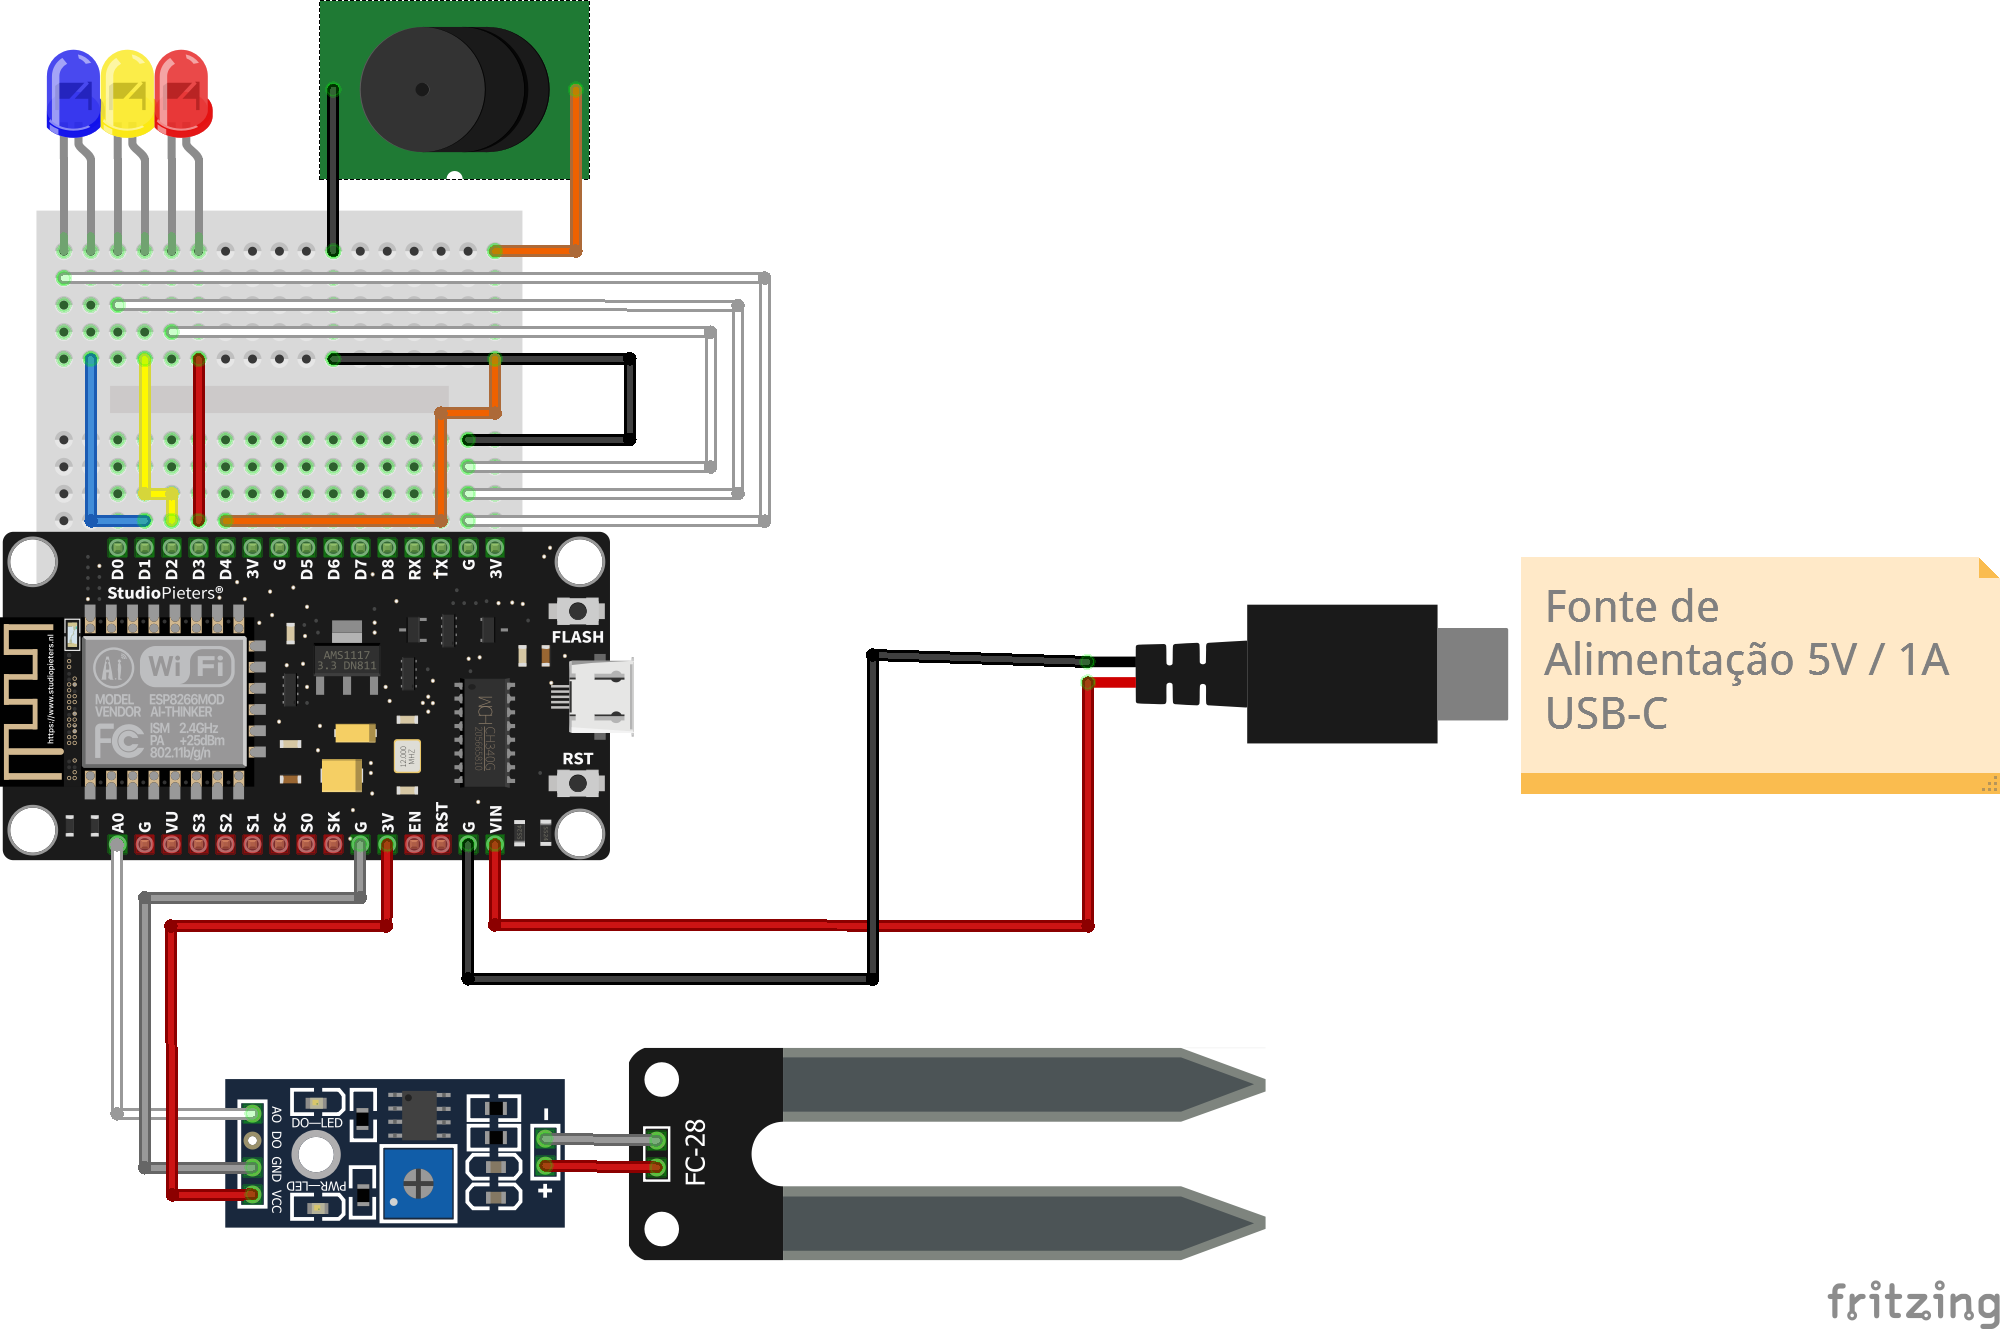
\includegraphics[width=0.85\textwidth]
    {figures/image51_componentes_ligados_versao_2_bb.png}
\caption{Diagrama de montagem do protótipo embarcado}
\label{fig:componentes_ligados}
\fonte{Elaborado pela autora no software Fritzing.}
\end{figure}

\begin{figure}[htb]
\centering
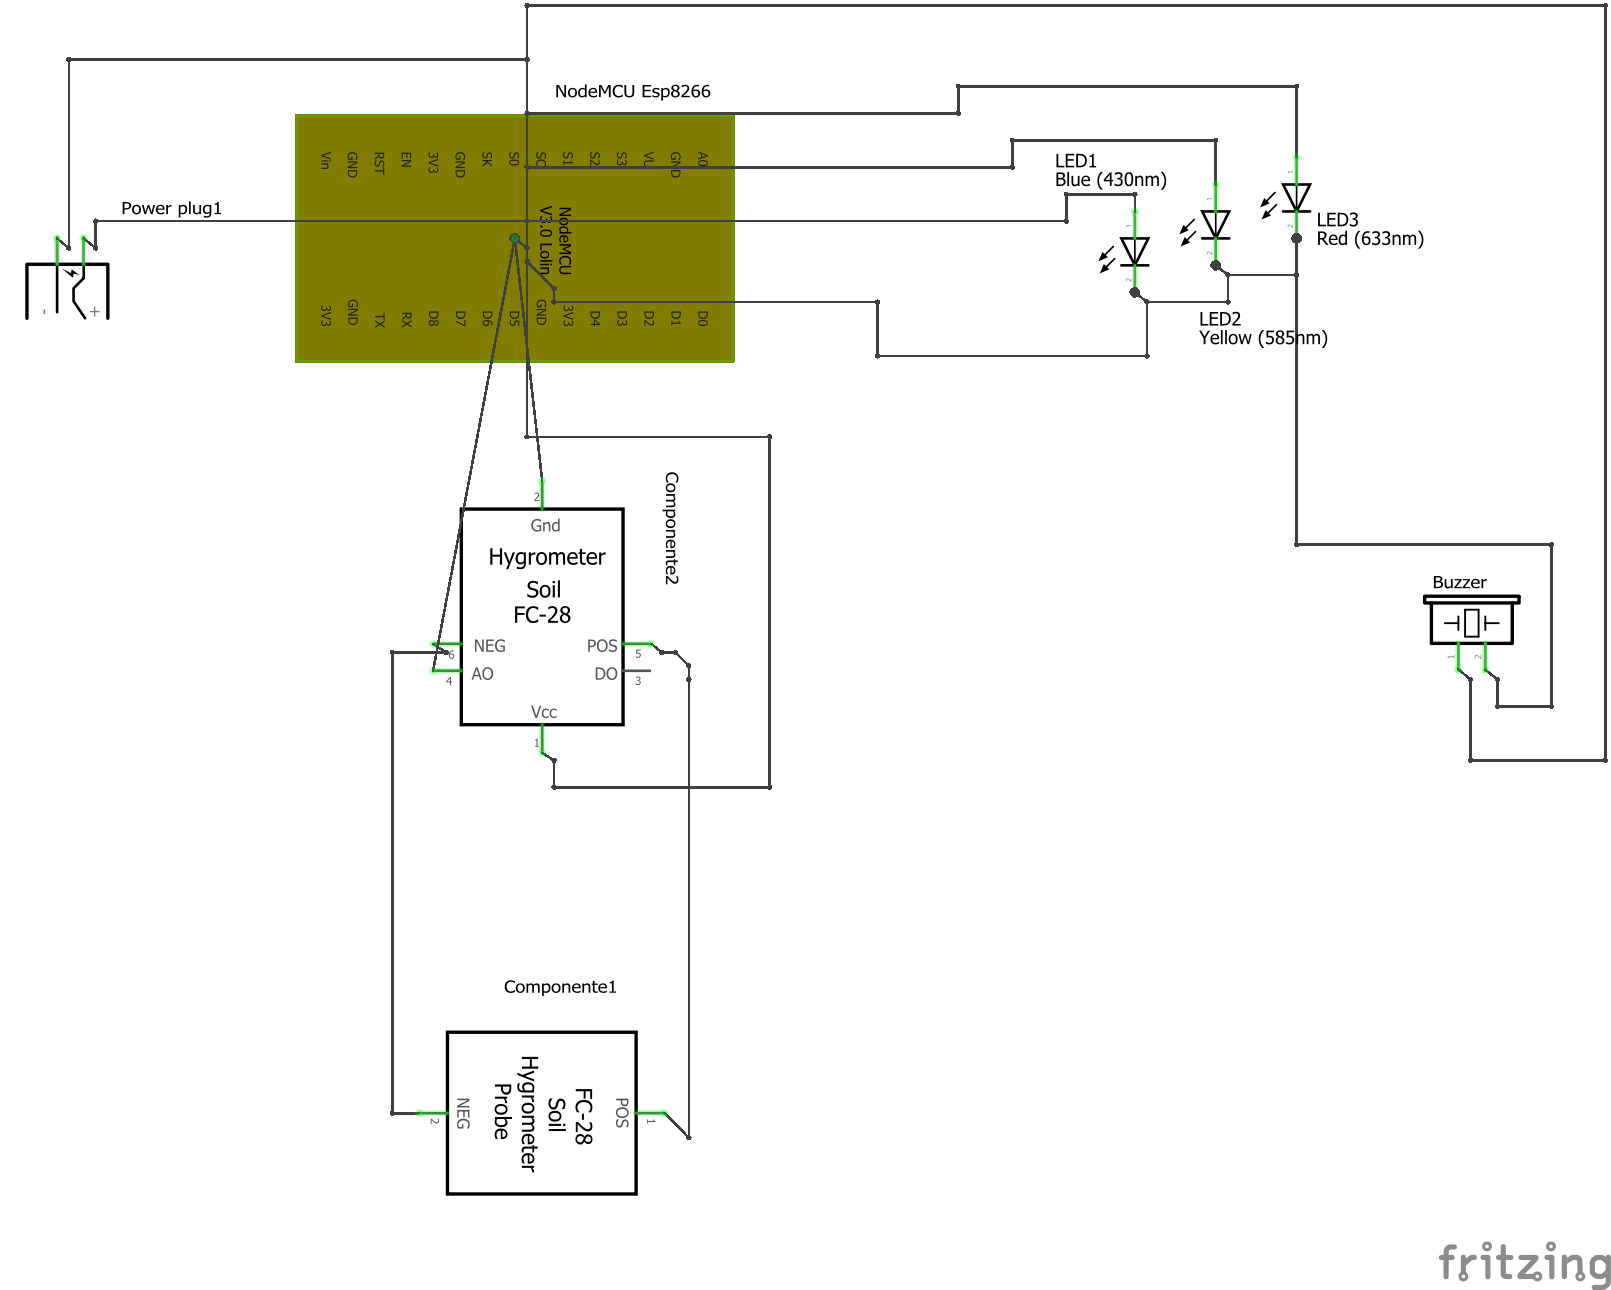
\includegraphics[width=0.85\textwidth]
    {figures/image52_componentes_ligados_versao_2_Esquematico.png}
\caption{Esquemático elétrico do protótipo embarcado}
\label{fig:esquematico}
\fonte{Elaborado pela autora no software Fritzing.}
\end{figure}

% -------------------------------------------------------------
\subsection{Especificações Técnicas e Custos}
\label{subsec:specs-custos}
% -------------------------------------------------------------

A Tabela~\ref{tab:specs} consolida as principais especificações
técnicas dos componentes utilizados.

\begin{table}[htb]
\centering
\caption{Especificações técnicas dos componentes do protótipo}
\label{tab:specs}
\begin{tabular}{llll}
\hline
\textbf{Componente}      & \textbf{Tensão (V)} & \textbf{Corrente máx.} & \textbf{Interface} \\
\hline
ESP8266 NodeMCU V3       & 3,3 (lógico)        & 200\,mA                & Wi-Fi / GPIO / ADC \\
Higrômetro LM393         & 3,3–5               & —                      & Analógica (A0)     \\
LED verde 5\,mm          & 3,0–3,3             & 20\,mA                 & GPIO digital       \\
LED amarelo 5\,mm        & 2,0–2,2             & 20\,mA                 & GPIO digital       \\
LED vermelho 5\,mm       & 1,8                 & 15\,mA                 & GPIO digital       \\
\textit{Buzzer} BPA5 5\,V & 5                  & 40\,mA                 & GPIO digital (PWM) \\
\hline
\end{tabular}
\fonte{Elaborado pela autora com base em \citeonline{mercadolivre_esp8266,eletrogate_higrometro,usinainfo_led_amarelo,usinainfo_led_vermelho,usinainfo_buzzer}.}
\end{table}

O custo total dos componentes do protótipo é de R\$\,70,30, conforme
detalhado na Tabela~\ref{tab:custos}.

\begin{table}[htb]
\centering
\caption{Componentes e custos do protótipo embarcado}
\label{tab:custos}
\begin{tabular}{lcc}
\hline
\textbf{Componente}              & \textbf{Qtd.} & \textbf{Custo (R\$)} \\
\hline
ESP8266 NodeMCU V3               & 1             & 59,90                \\
Higrômetro resistivo LM393       & 1             & 7,50                 \\
\textit{Buzzer} passivo BPA5 5\,V & 1            & 2,30                 \\
LEDs indicadores (conjunto)      & 1             & 0,60                 \\
\hline
\textbf{Total}                   &               & \textbf{70,30}       \\
\hline
\end{tabular}
\fonte{Elaborado pela autora.}
\end{table}

% =============================================================
\section{Fontes de Dados Meteorológicos}
\label{sec:fontes-dados}
% =============================================================

O sistema integra duas fontes externas de dados meteorológicos,
cada uma com papel específico no modelo de risco.

\subsection{API BNDMET/DECEA — Precipitação Histórica}
\label{subsec:bndmet}

A Base Nacional de Dados Meteorológicos e Climáticos (BNDMET),
operada pelo Departamento de Controle do Espaço Aéreo (DECEA), foi
selecionada como fonte primária de dados de precipitação histórica.
O acesso à API exigiu solicitação formal junto ao DECEA, com
apresentação de credenciais acadêmicas e justificativa técnica para
uso dos dados em pesquisa científica.

A estação selecionada para o estudo foi a D6594 (Alberto Flores),
integrante da rede ANA e localizada na região de Brumadinho (MG),
referência do maior acidente de barragem de rejeitos do Brasil em
termos de vítimas \cite{robertson2019feijaoson2019}. O acesso se dá pelo
\textit{endpoint} \texttt{/v1/estacoes/D6594/fenomenos/\{codigo\}},
com autenticação por chave estática (\textit{API key}) transmitida
no cabeçalho \texttt{x-api-key}.

Foram utilizados dois fenômenos da estação:

\begin{itemize}
    \item \textbf{I006} (precipitação diária acumulada) — consultado
    com janela de 30 dias para obter os acumulados de 24 horas, 7
    dias e 30 dias necessários ao modelo de risco;

    \item \textbf{I175} (precipitação horária) — consultado para
    identificação da precipitação observada mais próxima do instante
    atual, complementando o dado diário.
\end{itemize}

A escolha do BNDMET em detrimento da API HidroWebService da Agência
Nacional de Águas (ANA) foi motivada por uma restrição operacional
desta última: o campo \texttt{tokenautenticacao}, obrigatório em todas
as requisições da ANA, possui validade de apenas 60 minutos, exigindo
renovação periódica. Tal comportamento é incompatível com a operação
autônoma e contínua do ESP8266, que necessita de um mecanismo de
autenticação estável e de baixa complexidade. Como a estação D6594
já estava disponível via BNDMET com autenticação por chave estática,
a integração foi consolidada exclusivamente por essa interface.

\subsection{API OpenWeatherMap — Previsão e Dados Atuais}
\label{subsec:owm}

A API OpenWeatherMap (OWM) foi utilizada para obtenção de dois
conjuntos de dados complementares:

\begin{itemize}
    \item \textbf{\textit{Endpoint} \texttt{/weather}} — fornece
    as condições meteorológicas atuais, incluindo pressão atmosférica
    ao nível do solo (campo \texttt{grnd\_level}, em hPa), temperatura,
    umidade relativa do ar e precipitação na última hora;

    \item \textbf{\textit{Endpoint} \texttt{/forecast}} — fornece
    a previsão pluviométrica para as próximas 24 horas em blocos de
    3 horas (\texttt{cnt=8}), utilizada para o cálculo do componente
    de chuva futura do modelo de risco.
\end{itemize}

Ambos os \textit{endpoints} são acessados por HTTPS, com
autenticação por chave de API transmitida como parâmetro de
\textit{query}. As coordenadas utilizadas foram as da região de
Brumadinho — Córrego do Feijão
(latitude~$-$20,1433; longitude~$-$44,1997).

% =============================================================
\section{Modelo de Avaliação de Risco Integrado}
\label{sec:modelo-risco}
% =============================================================

O modelo de avaliação de risco quantifica, em cada ciclo de análise,
as condições geotécnicas e meteorológicas da estrutura monitorada
por meio de um índice numérico adimensional. O fator de risco integrado
($F_{risco}$) é calculado pela soma ponderada de sete variáveis,
conforme a Equação~\ref{eq:frisco}.

\begin{equation}
\label{eq:frisco}
F_{risco} = V_{len} + V_{ch.24h} + V_{ch.7d} + V_{ch.30d}
            + V_{ch.fut} + V_{taxa} + V_{press}
\end{equation}

\noindent onde cada variável representa uma dimensão do risco geotécnico
e meteorológico, descrita nas subseções seguintes.

% -------------------------------------------------------------
\subsection{Parâmetros Geotécnicos}
\label{subsec:geotecnicos}
% -------------------------------------------------------------

\subsubsection{Nível do Lençol Freático (\texorpdfstring{$V_{len}$}{V\_len})}

O nível do lençol freático é estimado indiretamente pela umidade do
solo medida pelo higrômetro. O fator de lençol freático
($F_{len}$) é calculado pela Equação~\ref{eq:flencol}:

\begin{equation}
\label{eq:flencol}
F_{len} = \frac{\text{Umidade}_{solo}\,(\%)}{25\,\%}
\end{equation}

O valor crítico de referência de 25\% corresponde à saturação máxima
do sensor para efeitos do modelo, com $F_{len}$ limitado ao intervalo
$[0;\,1]$. O peso atribuído a esta variável é de 0,40, o maior do
modelo, por ser o indicador mais direto da estabilidade do maciço.
A variável componente é obtida pela Equação~\ref{eq:vlen}:

\begin{equation}
\label{eq:vlen}
V_{len} = F_{len} \times 0{,}40
\end{equation}

Adicionalmente, quando a umidade do solo atinge o limiar de 30\%,
o sistema aciona imediatamente o protocolo de ruptura, forçando
$F_{risco} = 1{,}0$ independentemente dos demais parâmetros e
ativando o LED vermelho e o \textit{buzzer}.

\subsubsection{Taxa de Variação da Umidade (\texorpdfstring{$V_{taxa}$}{V\_taxa})}

A taxa de variação da umidade mensura a velocidade de saturação do
maciço ao longo do tempo, calculada a partir de um \textit{buffer}
circular de dez leituras consecutivas. O valor normalizado é obtido
pela Equação~\ref{eq:vtaxa}:

\begin{equation}
\label{eq:vtaxa}
V_{taxa} = \frac{|\Delta U|}{100\,\%} \times 0{,}10
\end{equation}

\noindent onde $|\Delta U|$ é o valor absoluto da variação percentual de umidade
entre a leitura mais recente e a mais antiga do \textit{buffer}. O uso do
valor absoluto garante que tanto a absorção quanto a drenagem rápida do solo
contribuam para o risco; a normalização por 100\% evita a saturação do
componente em eventos de variação extrema, preservando a escala proporcional.

% -------------------------------------------------------------
\subsection{Parâmetros Pluviométricos}
\label{subsec:pluviometricos}
% -------------------------------------------------------------

\subsubsection{Precipitação nas últimas 24 horas (\texorpdfstring{$V_{ch.24h}$}{V\_ch.24h})}

O limiar de 50\,mm em 24 horas foi estabelecido com base em dois
referenciais: o acidente de Merriespruit (África do Sul, 1994), no
qual precipitação de 50\,mm antecedeu o rompimento da barragem
\cite{rico2008mine}; e os critérios de alerta nível~3 do sistema
AlertaRio, que classifica precipitações acima de 50\,mm/24h como de
alto potencial de risco \cite{sistemaalertario2025}. A variável é calculada
pela Equação~\ref{eq:vch24h}:

\begin{equation}
\label{eq:vch24h}
V_{ch.24h} = \frac{\text{Precip}_{24h}\,\text{(mm)}}{50\,\text{mm}}
             \times 0{,}08
\end{equation}

\subsubsection{Precipitação acumulada nos últimos 7 dias (\texorpdfstring{$V_{ch.7d}$}{V\_ch.7d})}

O limiar de 150\,mm para a janela de 7 dias fundamenta-se em
\citeonline{rico2008mine}, que identificaram chuvas intensas como
principal causa de rompimentos na Europa (35\%) e causa global
relevante (25\%). O componente é dado pela Equação~\ref{eq:vch7d}:

\begin{equation}
\label{eq:vch7d}
V_{ch.7d} = \frac{\text{Precip}_{7d}\,\text{(mm)}}{150\,\text{mm}}
            \times 0{,}12
\end{equation}

\subsubsection{Precipitação acumulada nos últimos 30 dias (\texorpdfstring{$V_{ch.30d}$}{V\_ch.30d})}

O limiar de 300\,mm para 30 dias foi calibrado com base na análise
histórica dos dados da estação D6594. A análise por janela deslizante
de 30 dias consecutivos identificou o período de maior acúmulo em
cada temporada chuvosa: 346\,mm entre 2 e 31 de janeiro de 2026 e
310\,mm entre 5 de janeiro e 3 de fevereiro de 2025. O valor de
300\,mm representa, portanto, um limiar próximo ao pico histórico
observado na região. O componente é calculado pela
Equação~\ref{eq:vch30d}:

\begin{equation}
\label{eq:vch30d}
V_{ch.30d} = \frac{\text{Precip}_{30d}\,\text{(mm)}}{300\,\text{mm}}
             \times 0{,}10
\end{equation}

\subsubsection{Previsão de Intensidade Pluviométrica (\texorpdfstring{$V_{ch.fut}$}{V\_ch.fut})}

A previsão de precipitação para as próximas 24 horas é obtida via
OWM e classificada em cinco categorias de intensidade, conforme a
Tabela~\ref{tab:intensidade}. A variável utiliza um fator discreto
($F_{int}$) correspondente à classe identificada.

\begin{table}[htb]
\centering
\caption{Classificação da intensidade pluviométrica prevista e fator correspondente}
\label{tab:intensidade}
\begin{tabular}{lcc}
\hline
\textbf{Intensidade}     & \textbf{Acumulado previsto 24h (mm)} & \textbf{Fator ($F_{int}$)} \\
\hline
Fraca                    & $< 5$                                & 0,00                       \\
Moderada                 & $5 \leq x < 25$                      & 0,25                       \\
Forte                    & $25 \leq x < 50$                     & 0,50                       \\
Muito forte              & $50 \leq x < 80$                     & 0,75                       \\
Pancada de chuva         & $\geq 80$                            & 1,00                       \\
\hline
\end{tabular}
\fonte{Adaptado de \citeonline{sistemaalertario2025}.}
\end{table}

O componente é calculado pela Equação~\ref{eq:vchfut}:

\begin{equation}
\label{eq:vchfut}
V_{ch.fut} = F_{int} \times 0{,}15
\end{equation}

% -------------------------------------------------------------
\subsection{Parâmetro Atmosférico}
\label{subsec:atmosferico}
% -------------------------------------------------------------

\subsubsection{Queda de Pressão Atmosférica (\texorpdfstring{$V_{press}$}{V\_press})}

Quedas rápidas de pressão atmosférica sinalizam a aproximação de
frentes frias ou sistemas de baixa pressão associados a
precipitações intensas. O limiar de 5\,hPa em 3 horas foi adotado
como indicador de instabilidade atmosférica iminente. O componente
é calculado pela Equação~\ref{eq:vpress}:

\begin{equation}
\label{eq:vpress}
V_{press} = \frac{\max(\Delta P,\,0)}{5\,\text{hPa}} \times 0{,}05
\end{equation}

\noindent onde $\Delta P$ é a queda de pressão em hPa observada no
intervalo de 3 horas entre leituras consecutivas.

% -------------------------------------------------------------
\subsection{Distribuição de Pesos e Limites de Alerta}
\label{subsec:pesos-limites}
% -------------------------------------------------------------

A Tabela~\ref{tab:pesos} apresenta a distribuição de pesos das sete
variáveis do modelo. Os pesos somam 1,00, garantindo que $F_{risco}$
varie entre 0 e 1 em condições normais de operação.

\begin{table}[htb]
\centering
\caption{Variáveis do modelo de risco, fontes de dados e pesos atribuídos}
\label{tab:pesos}
\begin{tabular}{llcc}
\hline
\textbf{Variável} & \textbf{Fonte}                & \textbf{Peso} & \textbf{Limiar máx.} \\
\hline
$V_{len}$         & Higrômetro (sensor físico)    & 0,40          & Umidade $\geq 25\,\%$ \\
$V_{ch.24h}$      & BNDMET / I006                 & 0,08          & 50\,mm               \\
$V_{ch.7d}$       & BNDMET / I006                 & 0,12          & 150\,mm              \\
$V_{ch.30d}$      & BNDMET / I006                 & 0,10          & 300\,mm              \\
$V_{ch.fut}$      & OpenWeatherMap /forecast      & 0,15          & $\geq 80$\,mm/24h    \\
$V_{taxa}$        & Higrômetro (\textit{buffer} circular) & 0,10 & $|\Delta U| = 100\,\%$ \\
$V_{press}$       & OpenWeatherMap /weather       & 0,05          & Queda $\geq 5$\,hPa/3h \\
\hline
\textbf{Total}    &                               & \textbf{1,00} &                      \\
\hline
\end{tabular}
\fonte{Elaborado pela autora.}
\end{table}

Os limites de alerta e a sinalização correspondente são apresentados
na Tabela~\ref{tab:alertas}.

\begin{table}[htb]
\centering
\caption{Classificação do nível de alerta com base no fator de risco integrado}
\label{tab:alertas}
\begin{tabular}{ccc}
\hline
\textbf{Fator de Risco} & \textbf{LED} & \textbf{Situação}                       \\
\hline
$0{,}00 \leq F_{risco} \leq 0{,}45$ & Verde   & Condições normais de operação           \\
$0{,}46 \leq F_{risco} \leq 0{,}75$ & Amarelo & Atenção — monitoramento intensificado   \\
$F_{risco} > 0{,}75$                 & Vermelho & Alerta crítico — ação imediata requerida \\
\hline
\end{tabular}
\fonte{Elaborado pela autora.}
\end{table}

% -------------------------------------------------------------
\subsection{Mecanismo de Amplificação}
\label{subsec:amplificacao}
% -------------------------------------------------------------

O modelo incorpora um mecanismo de amplificação do fator de risco,
ativado quando duas condições são verificadas simultaneamente:
$F_{len} \geq 0{,}70$ (solo em estado avançado de saturação,
equivalente a umidade $\geq 17{,}5\,\%$) e acumulado previsto para
as próximas 24 horas classificado como moderado ou superior
($\geq 5$\,mm). Quando ambas as condições são satisfeitas, o fator
de risco calculado é multiplicado por 1,20, conforme a
Equação~\ref{eq:amplif}:

\begin{equation}
\label{eq:amplif}
F_{risco}^{*} = F_{risco} \times 1{,}20
\end{equation}

Esta abordagem é fundamentada no comportamento geotécnico observado
em acidentes históricos: em Brumadinho (2019), a barragem já
apresentava nível d'água interno elevado de forma persistente, e o
período foi precedido por chuvas intensas que reduziram a
resistência do material na zona acima do lençol freático
\cite{robertson2019feijaoson2019}.

% =============================================================
\section{Plataforma de \textit{Software}}
\label{sec:software}
% =============================================================

A plataforma de \textit{software} foi desenvolvida com arquitetura
cliente-servidor, organizada em três camadas: \textit{firmware}
embarcado, \textit{backend} e \textit{frontend}.

\subsection{Ambiente de Desenvolvimento}
\label{subsec:ambiente}

As tecnologias utilizadas no desenvolvimento estão listadas na
Tabela~\ref{tab:tecnologias}.

\begin{table}[htb]
\centering
\caption{Tecnologias utilizadas no desenvolvimento da plataforma}
\label{tab:tecnologias}
\begin{tabular}{lll}
\hline
\textbf{Camada}       & \textbf{Tecnologia}               & \textbf{Função}                           \\
\hline
\textit{Firmware}     & C++ / Arduino IDE                 & Lógica embarcada do ESP8266               \\
\textit{Firmware}     & ArduinoJson 6                     & Serialização e envio de dados JSON        \\
\textit{Backend}      & Node.js 20 + TypeScript           & Servidor de aplicação                     \\
\textit{Backend}      & Express.js                        & Roteamento e middlewares HTTP             \\
\textit{Backend}      & Prisma ORM                        & Mapeamento objeto-relacional              \\
\textit{Backend}      & PostgreSQL + TimescaleDB          & Banco de dados com suporte a séries temporais \\
\textit{Backend}      & Docker / Docker Compose           & Conteinerização e orquestração            \\
\textit{Frontend}     & React 18 + Next.js 14             & Interface web de monitoramento            \\
\textit{Frontend}     & Recharts                          & Visualização de dados em gráficos         \\
\textit{Frontend}     & Nodemailer                        & Envio de alertas por e-mail               \\
\hline
\end{tabular}
\fonte{Elaborado pela autora.}
\end{table}

\subsection{Arquitetura Modular do Sistema}
\label{subsec:arquitetura}

O sistema foi estruturado em três módulos funcionais, conforme
descrito a seguir.

O \textbf{Módulo de Aquisição de Dados} é responsável pela coleta
e transmissão das informações ao banco de dados. Compreende o
\textit{firmware} do ESP8266, que realiza leituras periódicas do
higrômetro e consulta as APIs do BNDMET e da OpenWeatherMap. Os
dados são serializados em JSON e enviados ao \textit{backend} via
requisição HTTP com intervalos adaptativos por nível de risco: leitura
do higrômetro a cada 30\,s (VERDE), 10\,s (AMARELO) ou 5\,s
(VERMELHO); envio ao \textit{backend} a cada 60\,s (VERDE),
20\,s (AMARELO) ou 10\,s (VERMELHO).

O \textbf{Módulo de Análise de Dados} executa o cálculo do fator
de risco integrado a partir dos dados recebidos, aplicando a
Equação~\ref{eq:frisco} e o mecanismo de amplificação quando
pertinente. O módulo também computa o índice de confiabilidade da
análise, reduzido proporcionalmente a falhas de sensor, indisponibilidade
de APIs ou insuficiência de dados históricos.

O \textbf{Módulo de Alerta} é responsável pelo acionamento dos
indicadores físicos (LEDs e \textit{buzzer}) e pelo envio de
notificações por e-mail quando o nível de risco ultrapassa os
limiares definidos. Os e-mails contêm o relatório do ciclo de
análise correspondente, incluindo os valores de cada componente
da equação de risco.

% =============================================================
\subsection{Modelagem UML}
\label{subsec:uml}
% =============================================================

A modelagem do sistema foi realizada por meio de diagramas UML
(\textit{Unified Modeling Language}), contemplando o diagrama de
casos de uso, o diagrama de classes e o diagrama de sequência. Esta
abordagem permite uma representação estruturada das funcionalidades,
das entidades de dados e dos fluxos de comunicação entre os
componentes \cite{sommerville2011engenharia,larman2007utilizando}.

% -------------------------------------------------------------
\subsubsection{Diagramas de Casos de Uso}
\label{subsubsec:casos-uso}
% -------------------------------------------------------------

O diagrama de casos de uso descreve as interações entre os atores do
sistema e as funcionalidades disponíveis. O sistema conta com seis atores:
três humanos — \textbf{Usuário Básico} (cadastra-se para receber alertas),
\textbf{Administrador} (responsável pelo monitoramento e gestão da
plataforma) e \textbf{Super Administrador} (herda todas as permissões do
Administrador e pode gerenciar outros administradores) — e três de sistema
— \textbf{ESP8266} (coleta e envia leituras), \textbf{API BNDMET} (fonte
de precipitação histórica) e \textbf{API OpenWeatherMap} (previsão
meteorológica e pressão atmosférica). Em razão do volume de
funcionalidades, os diagramas foram divididos em quatro partes,
detalhadas nas subseções a seguir.


\begin{figure}[htb]
\centering
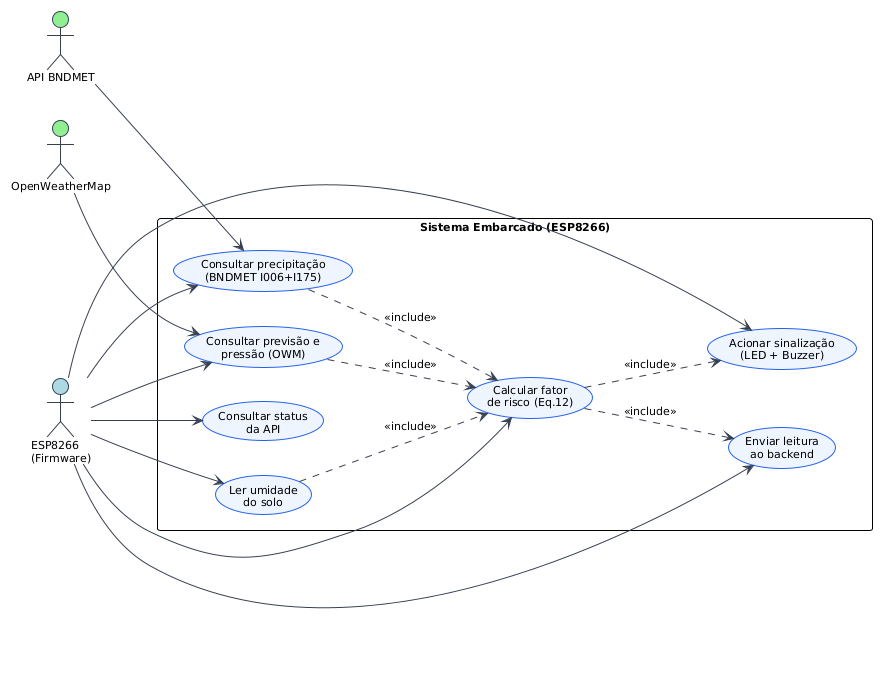
\includegraphics[width=1\textwidth]
    {figures/image53_diagrama_caso_de_uso_versao_3_pt1.png}
\caption{Diagrama de casos de uso --- Parte 1: Sistema Embarcado}
\label{fig:uc-parte1}
\fonte{Elaborado pela autora.}
\end{figure}

\begin{figure}[htb]
\centering
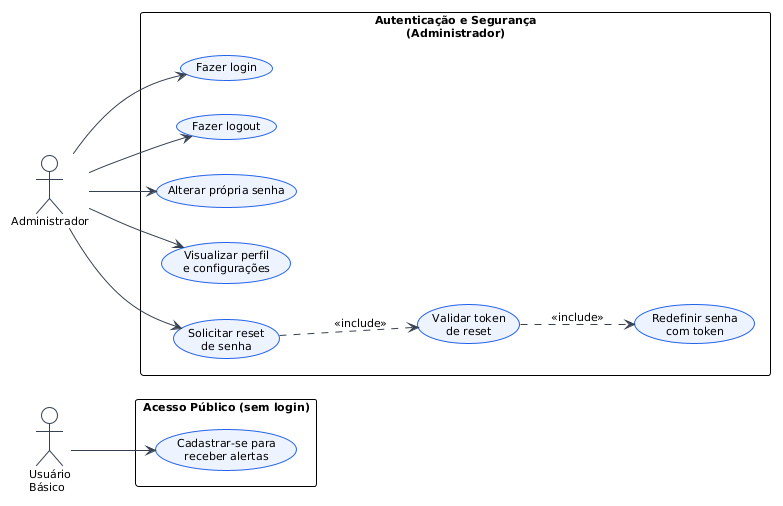
\includegraphics[width=1\textwidth]
    {figures/image53_diagrama_caso_de_uso_versao_3_pt2.png}
\caption{Diagrama de casos de uso --- Parte 2: Acesso Público e
Autenticação}
\label{fig:uc-parte2}
\fonte{Elaborado pela autora.}
\end{figure}

\begin{figure}[htb]
\centering
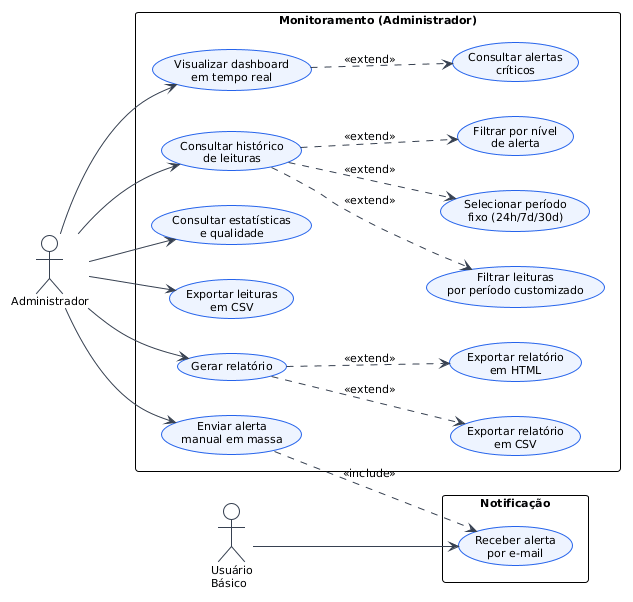
\includegraphics[width=1\textwidth]
    {figures/image53_diagrama_caso_de_uso_versao_3_pt3.png}
\caption{Diagrama de casos de uso --- Parte 3: Monitoramento e
Alertas}
\label{fig:uc-parte3}
\fonte{Elaborado pela autora.}
\end{figure}

\begin{figure}[htb]
\centering
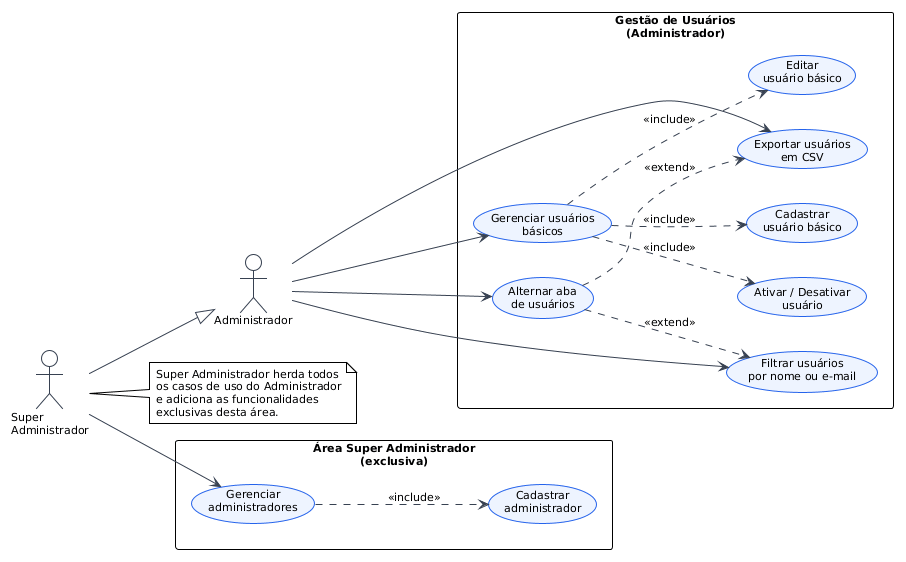
\includegraphics[width=1\textwidth]
    {figures/image53_diagrama_caso_de_uso_versao_3_pt4.png}
\caption{Diagrama de casos de uso --- Parte 4: Gestão de Usuários e
Área Super Administrador}
\label{fig:uc-parte4}
\fonte{Elaborado pela autora.}
\end{figure}

% ══════════════════════════════════════════════════════════════
\paragraph{Parte 1 --- Sistema Embarcado (ESP8266)}\hfill\break
% ══════════════════════════════════════════════════════════════

% ─────────────────────────────────────────────────────────────
\paragraph{UC01 --- Enviar leitura ao \textit{backend}}\hfill\break

\textbf{Ator Principal:} ESP8266 (Firmware).

\textbf{Interessado e Interesse:}

\textit{Backend} Node.js: receber, validar e persistir a leitura
completa do ciclo de monitoramento.

Administrador: consumir os dados registrados via
\textit{dashboard} e tela de sensores.

\textbf{Pré-condição:} dispositivo conectado à rede Wi-Fi; endereço
\texttt{192.168.1.108:3001} acessível na rede local; NTP
sincronizado com data posterior a 2001.

\textbf{Cenário de Sucesso Principal (Fluxo Básico):}
\begin{enumerate}
  \item O \textit{firmware} lê a umidade do solo via ADC no pino A0
        e mapeia o valor bruto (0--1023) para o intervalo 0--100\%
        utilizando os parâmetros \texttt{SENSOR\_SECO} e
        \texttt{SENSOR\_UMIDO} persistidos na EEPROM.
  \item O sistema consulta a API BNDMET via HTTPS com cabeçalho
        \texttt{x-api-key}, obtendo precipitação acumulada
        (fenômeno I006, janela de 30 dias) e precipitação horária
        (fenômeno I175, dia corrente).
  \item O sistema consulta a API OpenWeatherMap via HTTPS no
        \textit{endpoint} \texttt{/weather} para obter pressão
        atmosférica ao nível do solo (\texttt{grnd\_level}) e
        precipitação na última hora (\texttt{rain.1h}); em seguida
        consulta \texttt{/forecast} com \texttt{cnt=8} para a
        previsão pluviométrica das próximas 24 horas em blocos
        de 3 horas.
  \item O sistema calcula o fator de risco integrado pela
        Equação~\ref{eq:frisco}, aplicando o mecanismo de
        amplificação $\times 1{,}20$ se $F_{len} \geq 0{,}70$
        e \texttt{chuvaFutura24h} $\geq 5$\,mm/24h.
  \item O sistema classifica o nível de alerta (VERDE, AMARELO
        ou VERMELHO) e aciona o LED e o \textit{buzzer}
        correspondentes.
  \item O \textit{firmware} serializa os dados em JSON com
        aproximadamente 35 campos e envia via
        \texttt{POST /api/sensor/dados} com cabeçalho
        \texttt{Content-Type: application/json}.
  \item O \textit{backend} persiste a leitura em
        \texttt{leituras\_sensor} e retorna HTTP 201 com
        \texttt{\{"success": true\}}.
  \item O \textit{firmware} define \texttt{apiConectada = true}
        e zera o contador \texttt{tentativasEnvioAPI}.
\end{enumerate}

\textbf{Extensões (Fluxo Alternativo):}

\begin{enumerate}
  \renewcommand{\theenumi}{1a}
  \renewcommand{\labelenumi}{\theenumi.}
  \item Umidade do solo atinge ou supera 30\% (ruptura imediata)
  \begin{enumerate}
  \item O sistema chama \texttt{acionarRuptura()} antes do
        cálculo completo, forçando \texttt{riscoIntegrado = 1{,}0},
        \texttt{nivelAlerta = VERMELHO} e
        \texttt{statusTexto = RUPTURA}.
  \item O LED vermelho e o \textit{buzzer} são acionados
        imediatamente com frequência de 2400\,Hz.
  \item O sistema retorna ao passo 6 do fluxo básico com os
        valores de ruptura.
  \end{enumerate}
\end{enumerate}

\begin{enumerate}
  \renewcommand{\theenumi}{1b}
  \renewcommand{\labelenumi}{\theenumi.}
  \item Umidade retorna abaixo de 30\% após ruptura
  \begin{enumerate}
  \item O sistema aguarda três leituras consecutivas seguras
        via \texttt{contagemRetornoRuptura} antes de recalcular
        normalmente.
  \item Durante esse período, \texttt{aguardandoResetRuptura = true}
        é serializado no JSON enviado ao \textit{backend}.
  \item O sistema retorna ao passo 4 do fluxo básico.
  \end{enumerate}
\end{enumerate}

\begin{enumerate}
  \renewcommand{\theenumi}{2a}
  \renewcommand{\labelenumi}{\theenumi.}
  \item BNDMET indisponível no passo 2
  \begin{enumerate}
  \item O sistema define \texttt{apiDisponivel = false} e
        reduz o intervalo de \textit{retry} para 30 segundos
        (\texttt{INTERVALO\_RETRY\_API\_FALHA}).
  \item Os componentes $V_{ch.24h}$, $V_{ch.7d}$ e $V_{ch.30d}$
        recebem valor zero e a confiabilidade é descontada em
        25 pontos.
  \item O sistema retorna ao passo 3 do fluxo básico.
  \end{enumerate}
\end{enumerate}

\begin{enumerate}
  \renewcommand{\theenumi}{2b}
  \renewcommand{\labelenumi}{\theenumi.}
  \item NTP não sincronizado no passo 2
  \begin{enumerate}
  \item A consulta ao BNDMET é adiada e registrada no Serial
        como \textit{``NTP ainda não sincronizado''}.
  \item O sistema retorna ao passo 3 do fluxo básico sem
        consultar o BNDMET.
  \end{enumerate}
\end{enumerate}

\begin{enumerate}
  \renewcommand{\theenumi}{3a}
  \renewcommand{\labelenumi}{\theenumi.}
  \item OpenWeatherMap indisponível no passo 3
  \begin{enumerate}
  \item O \texttt{timestamp} do OWM não é atualizado;
        \texttt{vChuvaFutura} e \texttt{vPressao} recebem
        valor zero.
  \item A confiabilidade é descontada em 15 pontos.
  \item O sistema retorna ao passo 4 do fluxo básico.
  \end{enumerate}
\end{enumerate}

\begin{enumerate}
  \renewcommand{\theenumi}{6a}
  \renewcommand{\labelenumi}{\theenumi.}
  \item Wi-Fi desconectado no passo 6
  \begin{enumerate}
  \item O envio é abortado e registrado no Serial.
  \item O sistema tenta reconectar via \texttt{WiFi.reconnect()}
        a cada 30 segundos.
  \item Após 10 tentativas sem sucesso, o ESP8266 reinicia
        via \texttt{ESP.restart()}.
  \end{enumerate}
\end{enumerate}

\begin{enumerate}
  \renewcommand{\theenumi}{6b}
  \renewcommand{\labelenumi}{\theenumi.}
  \item \textit{Backend} não responde no passo 6
  \begin{enumerate}
  \item O contador \texttt{tentativasEnvioAPI} é incrementado.
  \item Após 10 falhas consecutivas, o módulo Wi-Fi é
        desconectado e reconectado.
  \end{enumerate}
\end{enumerate}

\begin{enumerate}
  \renewcommand{\theenumi}{8a}
  \renewcommand{\labelenumi}{\theenumi.}
  \item Heap crítico detectado após o passo 8
  \begin{enumerate}
  \item Se \texttt{ESP.getFreeHeap()} $<$ 5000 bytes, o sistema
        reinicia automaticamente via \texttt{ESP.restart()}.
  \end{enumerate}
\end{enumerate}

\textbf{Pós-Condições:} leitura persistida em
\texttt{leituras\_sensor} com todos os campos do ciclo de análise;
\texttt{apiConectada = true}; sinalização visual e sonora atualizada.

\textbf{Requisitos especiais:} conectividade Wi-Fi na rede local;
certificados HTTPS aceitos via \texttt{setInsecure()} para BNDMET
e OWM.

\textbf{Frequência:} a cada 10--60 segundos, adaptativo por nível de
risco: 60\,s (VERDE), 20\,s (AMARELO) e 10\,s (VERMELHO).

% ─────────────────────────────────────────────────────────────
\paragraph{UC02 --- Calcular fator de risco}\hfill\break

\textbf{Ator Principal:} ESP8266 (Firmware).

\textbf{Interessado e Interesse:}

ESP8266: determinar o nível de risco atual para acionar a
sinalização correta e compor o JSON enviado ao \textit{backend}.

\textbf{Pré-condição:} pelo menos uma leitura do higrômetro
realizada; estruturas \texttt{dadosLocais}, \texttt{dadosBNDMET},
\texttt{dadosMeteo} e \texttt{previsao} inicializadas.

\textbf{Cenário de Sucesso Principal (Fluxo Básico):}
\begin{enumerate}
  \item O sistema calcula cada componente individualmente:
        $V_{len}$, $V_{ch.24h}$, $V_{ch.7d}$, $V_{ch.30d}$,
        $V_{ch.fut}$, $V_{taxa}$ e $V_{press}$.
  \item O sistema soma os componentes para obter
        \texttt{riscoIntegrado} pela Equação~\ref{eq:frisco}.
  \item O sistema verifica as condições de amplificação:
        se $F_{len} \geq 0{,}70$ e previsão $\geq 5$\,mm/24h,
        aplica o coeficiente $\times 1{,}20$.
  \item O sistema classifica o nível por faixa: VERDE
        ($\leq 0{,}45$), AMARELO ($\leq 0{,}75$) ou VERMELHO
        ($> 0{,}75$).
  \item O sistema calcula o índice de confiabilidade,
        descontando pontos por: sensor com falha ($-40$),
        BNDMET indisponível ($-25$), OWM indisponível ($-15$),
        Wi-Fi desconectado ($-10$), \textit{buffer} insuficiente
        ($-10$) e qualidade BNDMET $< 80$\% ($-10$).
  \item O sistema gera a mensagem de recomendação operacional
        com base no nível, na previsão e na disponibilidade
        das APIs.
  \item O sistema atualiza os históricos circulares
        \texttt{historicoRisco[10]} e \\
        \texttt{historicoUmidade[10]}.
\end{enumerate}

\textbf{Extensões (Fluxo Alternativo):}

\begin{enumerate}
  \renewcommand{\theenumi}{5a}
  \renewcommand{\labelenumi}{\theenumi.}
  \item Estado de ruptura ativa no passo 5
  \begin{enumerate}
  \item A confiabilidade é fixada em 100\% independentemente
        de qualquer outra falha.
  \item O sistema retorna ao passo 6 do fluxo básico.
  \end{enumerate}
\end{enumerate}

\textbf{Pós-Condições:} estrutura \texttt{analiseRisco} populada
com fator integrado, nível de alerta, confiabilidade, todos os
componentes individuais e recomendação operacional.

\textbf{Requisitos especiais:} Nenhum.

\textbf{Frequência:} a cada ciclo de leitura do sensor.

% ─────────────────────────────────────────────────────────────
\paragraph{UC03 --- Acionar sinalização}\hfill\break

\textbf{Ator Principal:} ESP8266 (Firmware).

\textbf{Interessado e Interesse:}

Operador local: receber indicação visual e sonora imediata do
nível de risco sem necessidade de acesso à plataforma \textit{web}.

\textbf{Pré-condição:} \texttt{analiseRisco.nivelAlerta} calculado
pelo UC02; \texttt{modoManual = false}.

\textbf{Cenário de Sucesso Principal (Fluxo Básico):}
\begin{enumerate}
  \item O sistema desliga todos os LEDs e o \textit{buzzer}.
  \item O sistema aciona o LED correspondente ao nível: verde
        (pino D1) para VERDE, amarelo (D2) para AMARELO,
        vermelho (D3) para VERMELHO.
  \item No nível VERMELHO, o sistema ativa o \textit{buzzer}
        com frequência variável: 2000\,Hz para índice 80--84\%,
        2200\,Hz para 85--89\% e 2400\,Hz para $\geq 90$\%,
        com intervalos de \textit{beep} de 1000\,ms, 800\,ms,
        500\,ms e 300\,ms respectivamente.
\end{enumerate}

\textbf{Extensões (Fluxo Alternativo):}

\begin{enumerate}
  \renewcommand{\theenumi}{1a}
  \renewcommand{\labelenumi}{\theenumi.}
  \item Modo manual ativo no passo 1
  \begin{enumerate}
  \item O hardware não é alterado; o estado é mantido como
        definido pelo operador via Serial.
  \item O sistema encerra sem executar os demais passos.
  \end{enumerate}
\end{enumerate}

\begin{enumerate}
  \renewcommand{\theenumi}{2a}
  \renewcommand{\labelenumi}{\theenumi.}
  \item Ruptura ativa detectada antes do passo 2
  \begin{enumerate}
  \item O LED vermelho e o \textit{buzzer} são acionados
        diretamente por \texttt{acionarRuptura()}, sem passar
        pelo fluxo normal de \texttt{controlarSistemaFisico()}.
  \end{enumerate}
\end{enumerate}

\textbf{Pós-Condições:} LED e \textit{buzzer} refletem o nível
de risco atual do ciclo de análise.

\textbf{Requisitos especiais:} Nenhum.

\textbf{Frequência:} a cada ciclo de leitura do sensor.

% ─────────────────────────────────────────────────────────────
\paragraph{UC04 --- Consultar precipitação (BNDMET)}\hfill\break

\textbf{Ator Principal:} ESP8266 (Firmware).

\textbf{Interessado e Interesse:}

API BNDMET: fornecer dados pluviométricos históricos da estação
D6594 (Alberto Flores) para uso no modelo de risco.

\textbf{Pré-condição:} Wi-Fi conectado; NTP sincronizado com
data posterior a 2001.

\textbf{Cenário de Sucesso Principal (Fluxo Básico):}
\begin{enumerate}
  \item O sistema gera as datas de início (30 dias atrás) e
        fim (ontem) no formato \texttt{YYYY-MM-DD} via NTP.
  \item O sistema envia
        \path{GET https://api-bndmet.decea.mil.br/v1/%
        estacoes/D6594/fenomenos/I006?dataInicio=\&dataFinal=}
        com cabeçalho \texttt{x-api-key}.
  \item O sistema parseia o \textit{array} \texttt{data.data}
        de pares \texttt{[timestamp\_ms, valor]}, acumulando
        os valores dos últimos 7 e 30 dias e identificando
        o valor de ontem para \texttt{precipitacao24h}.
  \item O sistema calcula \texttt{qualidadeDados} como
        percentual de medições não nulas retornadas.
  \item O sistema envia
        \path{GET .../fenomenos/I175?dataInicio=hoje\&%
        dataFinal=hoje} e seleciona a medição com menor
        diferença em relação ao horário atual.
\end{enumerate}

\textbf{Extensões (Fluxo Alternativo):}

\begin{enumerate}
  \renewcommand{\theenumi}{2a}
  \renewcommand{\labelenumi}{\theenumi.}
  \item HTTP diferente de 200 no passo 2
  \begin{enumerate}
  \item O sistema define \texttt{apiDisponivel = false} e
        \texttt{statusAPI = ``FALHA''}.
  \item O intervalo de próxima consulta é reduzido para
        30 segundos.
  \end{enumerate}
\end{enumerate}

\begin{enumerate}
  \renewcommand{\theenumi}{2b}
  \renewcommand{\labelenumi}{\theenumi.}
  \item JSON malformado no passo 2
  \begin{enumerate}
  \item O sistema registra o erro no Serial e define
        \texttt{apiDisponivel = false}.
  \end{enumerate}
\end{enumerate}

\begin{enumerate}
  \renewcommand{\theenumi}{5a}
  \renewcommand{\labelenumi}{\theenumi.}
  \item Nenhuma medição retornada pelo I175 no passo 5
  \begin{enumerate}
  \item O sistema define \texttt{precipitacaoAtual = 0{,}0}.
  \end{enumerate}
\end{enumerate}

\textbf{Pós-Condições:} campos \texttt{precipitacao24h},
\texttt{precipitacao7d}, \texttt{precipitacao30d},
\texttt{precipitacaoAtual} e \texttt{qualidadeDados} populados
em \texttt{dadosBNDMET}.

\textbf{Requisitos especiais:} chave de API BNDMET válida
(\texttt{x-api-key}); NTP sincronizado para geração correta
das datas.

\textbf{Frequência:} a cada ciclo do \textit{loop} conforme
intervalo adaptativo por nível de risco; a cada 30 segundos
em caso de falha (\textit{retry} acelerado).

% ─────────────────────────────────────────────────────────────
\paragraph{UC05 --- Consultar previsão e pressão (OWM)}\hfill\break

\textbf{Ator Principal:} ESP8266 (Firmware).

\textbf{Interessado e Interesse:}

API OpenWeatherMap: fornecer dados de pressão atmosférica atual
e previsão pluviométrica para as próximas 24 horas.

\textbf{Pré-condição:} Wi-Fi conectado; chave de API OWM válida.

\textbf{Cenário de Sucesso Principal (Fluxo Básico):}
\begin{enumerate}
  \item O sistema envia \path{GET https://pro.openweather%
        map.org/data/2.5/weather?lat=-20.1433\&lon=-44.1997%
        \&appid=...\&units=metric\&lang=pt\_br} via HTTPS.
  \item O sistema extrai \texttt{grnd\_level} como pressão
        em hPa; se ausente, utiliza \texttt{pressure}; valida
        que o valor está no intervalo 700--1100\,hPa.
  \item O sistema calcula a queda de pressão em relação à
        leitura anterior no histórico circular de 6 pontos
        (janela de 3 horas).
  \item O sistema envia \path{GET .../forecast?cnt=8} e
        soma os campos \texttt{rain.3h} dos 8 blocos; quando
        \texttt{rain.3h} está ausente, utiliza
        \texttt{pop $\times$ 3{,}0} como estimativa.
  \item O sistema classifica \texttt{intensidadePrevisao} em
        Fraca, Moderada, Forte, Muito Forte ou Pancada de
        Chuva conforme a Tabela~\ref{tab:intensidade}.
\end{enumerate}

\textbf{Extensões (Fluxo Alternativo):}

\begin{enumerate}
  \renewcommand{\theenumi}{1a}
  \renewcommand{\labelenumi}{\theenumi.}
  \item HTTP diferente de 200 no passo 1
  \begin{enumerate}
  \item O \texttt{timestamp} do OWM não é atualizado;
        na próxima verificação o intervalo de \textit{retry}
        é reduzido para 30 segundos.
  \end{enumerate}
\end{enumerate}

\begin{enumerate}
  \renewcommand{\theenumi}{2a}
  \renewcommand{\labelenumi}{\theenumi.}
  \item Pressão fora do intervalo válido no passo 2
  \begin{enumerate}
  \item O valor é descartado e \texttt{vPressao} recebe zero.
  \end{enumerate}
\end{enumerate}

\begin{enumerate}
  \renewcommand{\theenumi}{0a}
  \renewcommand{\labelenumi}{\theenumi.}
  \item OWM ainda não consultada com sucesso desde o boot
  \begin{enumerate}
  \item A disponibilidade da OWM é inferida pelo campo
        \texttt{dadosMeteo.timestamp}: enquanto nenhuma consulta
        bem-sucedida ocorreu, \texttt{timestamp = 0} e o sistema
        trata a OWM como indisponível, aplicando desconto de
        $-15\%$ na confiabilidade e usando \textit{retry} de 30
        segundos. Essa condição é transitória e ocorre nos
        primeiros ciclos após o boot, mesmo quando a rede está
        disponível.
  \end{enumerate}
\end{enumerate}

\textbf{Pós-Condições:} campos \texttt{pressaoAtmosferica},
\texttt{chuvaFutura24h}, \\ \texttt{intensidadePrevisao} e
\texttt{fatorIntensidade} populados em \texttt{dadosMeteo}
e \texttt{previsao}.

\textbf{Requisitos especiais:} chave de API OWM válida com
acesso ao plano Pro (\texttt{pro.openweathermap.org}).

\textbf{Frequência:} \texttt{/weather} consultado a cada 10 minutos;
\texttt{/forecast} consultado a cada 30 minutos; ambos com
\textit{retry} acelerado a cada 30 segundos em caso de falha.
Os dois \textit{timers} são independentes entre si e em relação
ao nível de alerta vigente.

% ─────────────────────────────────────────────────────────────
\paragraph{UC06 --- Consultar status da API}\hfill\break

\textbf{Ator Principal:} ESP8266 (Firmware).

\textbf{Interessado e Interesse:}

ESP8266: verificar a disponibilidade do \textit{backend} local
antes de tentar enviar leituras.

\textbf{Pré-condição:} Wi-Fi conectado.

\textbf{Cenário de Sucesso Principal (Fluxo Básico):}
\begin{enumerate}
  \item O sistema envia
        \path{GET http://192.168.1.108:3001/api/sensor/status}.
  \item O \textit{backend} retorna HTTP 200.
  \item O sistema define \texttt{apiConectada = true}.
\end{enumerate}

\textbf{Extensões (Fluxo Alternativo):}

\begin{enumerate}
  \renewcommand{\theenumi}{1a}
  \renewcommand{\labelenumi}{\theenumi.}
  \item \textit{Backend} não responde no passo 1
  \begin{enumerate}
  \item O sistema define \texttt{apiConectada = false} e
        registra a falha no Serial.
  \end{enumerate}
\end{enumerate}

\textbf{Pós-Condições:} variável \texttt{apiConectada} atualizada
com o estado real do \textit{backend}.

\textbf{Requisitos especiais:} Nenhum.

\textbf{Frequência:} executado na inicialização do sistema e a
cada verificação de conectividade (a cada 30 segundos).

% ══════════════════════════════════════════════════════════════
\paragraph{Parte 2 --- Acesso Público e Autenticação}\hfill\break
% ══════════════════════════════════════════════════════════════

% ─────────────────────────────────────────────────────────────
\paragraph{UC07 --- Cadastrar-se para receber alertas}\hfill\break

\textbf{Ator Principal:} Usuário Básico.

\textbf{Interessado e Interesse:}

Usuário Básico: registrar seus dados para receber notificações
de alerta por e-mail quando o Administrador disparar um alerta.

Administrador: dispor de uma lista de destinatários cadastrados
para o envio de alertas em massa.

\textbf{Pré-condição:} nenhuma; rota pública
\texttt{POST /auth/cadastro-basico} sem autenticação.

\textbf{Cenário de Sucesso Principal (Fluxo Básico):}
\begin{enumerate}
  \item O Usuário Básico acessa a \textit{landing page} e
        clica em ``Cadastrar para Receber Alertas''.
  \item O sistema exibe o modal de cadastro com os campos:
        nome completo, e-mail, telefone (com máscara automática
        \texttt{(XX) XXXXX-XXXX}) e preferência de notificação
        (e-mail ou e-mail + SMS).
  \item O ator preenche os campos obrigatórios (nome, e-mail e telefone)
        e opcional (tipo de notificação).
  \item O ator clica em ``Cadastrar''.
  \item O sistema valida nome (2--100 caracteres), e-mail
        (formato válido) e telefone (formato brasileiro,
        se informado).
  \item O \textit{frontend} envia
        \texttt{POST /auth/cadastro-basico} com
        \texttt{\{nome, email, telefone, receberNotificacoes:
        true, tipoNotificacao\}}.
  \item O \textit{backend} verifica a unicidade do e-mail
        em \texttt{usuarios\_basicos} e cria o registro com
        \texttt{ativo = true}.
  \item O sistema fecha o modal, limpa o formulário e exibe
        \textit{toast}: ``Cadastro realizado com sucesso!
        Você receberá notificações sobre os alertas de
        barragem.''.
\end{enumerate}

\textbf{Extensões (Fluxo Alternativo):}

\begin{enumerate}
  \renewcommand{\theenumi}{5a}
  \renewcommand{\labelenumi}{\theenumi.}
  \item Campos obrigatórios não preenchidos no passo 5
  \begin{enumerate}
  \item O sistema exibe mensagens de erro inline em cada
        campo inválido via \textit{react-hook-form}.
  \item O botão ``Cadastrar'' permanece habilitado.
  \item O sistema retorna ao passo 3 do fluxo básico.
  \end{enumerate}
\end{enumerate}

\begin{enumerate}
  \renewcommand{\theenumi}{7a}
  \renewcommand{\labelenumi}{\theenumi.}
  \item E-mail já cadastrado no passo 7
  \begin{enumerate}
  \item O \textit{backend} retorna HTTP 400.
  \item O sistema exibe \textit{toast} de erro com a
        mensagem retornada pela API.
  \item O sistema retorna ao passo 3 do fluxo básico.
  \end{enumerate}
\end{enumerate}

\textbf{Pós-Condições:} registro criado em
\texttt{usuarios\_basicos} com \texttt{ativo = true} e
preferências de notificação salvas.

\textbf{Requisitos especiais:} Nenhum.

\textbf{Frequência:} Ocasionalmente.

% ─────────────────────────────────────────────────────────────
\paragraph{UC08 --- Fazer \textit{login}}\hfill\break

\textbf{Ator Principal:} Administrador.

\textbf{Interessado e Interesse:}

Administrador: autenticar-se para acessar o painel de
monitoramento e gestão da plataforma.

\textbf{Pré-condição:} conta existente em
\texttt{usuarios\_admin} com \texttt{ativo = true}.

\textbf{Cenário de Sucesso Principal (Fluxo Básico):}
\begin{enumerate}
  \item O Administrador acessa a \textit{landing page} e
        clica em ``Login''.
  \item O sistema exibe o modal de login com os campos:
        e-mail e senha.
  \item O ator clica em ``Entrar no Sistema''.
  \item O \textit{frontend} envia
        \texttt{POST /auth/login} com \texttt{\{email, senha\}}.
  \item O \textit{backend} busca o usuário em
        \texttt{usuarios\_admin} com \texttt{ativo = true}
        e valida a senha via \textit{bcrypt}.
  \item O \textit{backend} gera um token JWT com expiração de 24 horas,
        persiste a sessão em \texttt{sessoes\_usuario} com token, IP e
        agente de usuário, e atualiza \texttt{ultimoLogin}. Retorna
        HTTP~200 com \texttt{\{token, usuario, expiresAt\}}.
  \item O \textit{frontend} armazena o token e os dados do usuário no
        \texttt{localStorage} e no contexto React, e redireciona
        para \texttt{/dashboard}.
\end{enumerate}

\textbf{Extensões (Fluxo Alternativo):}

\begin{enumerate}
  \renewcommand{\theenumi}{4a}
  \renewcommand{\labelenumi}{\theenumi.}
  \item Credenciais inválidas no passo 4
  \begin{enumerate}
  \item O \textit{backend} retorna HTTP 401 com
        ``Credenciais inválidas'', sem especificar qual
        campo está incorreto.
  \item O sistema exibe mensagem de erro na tela de
        \textit{login}.
  \item O sistema retorna ao passo 1 do fluxo básico.
  \end{enumerate}
\end{enumerate}

\begin{enumerate}
  \renewcommand{\theenumi}{4b}
  \renewcommand{\labelenumi}{\theenumi.}
  \item Conta inativa no passo 4
  \begin{enumerate}
  \item A busca com \texttt{ativo: true} não localiza o
        usuário; o sistema retorna o mesmo erro de
        credenciais inválidas do passo 4a.
  \end{enumerate}
\end{enumerate}

\begin{enumerate}
  \renewcommand{\theenumi}{9a}
  \renewcommand{\labelenumi}{\theenumi.}
  \item Token expirado em uso posterior ao passo 9
  \begin{enumerate}
  \item O \textit{middleware} \texttt{verificarAutenticacao}
        rejeita a requisição com HTTP 401.
  \item O \textit{frontend} remove o token do
        \texttt{localStorage} e redireciona para
        \texttt{/login}.
  \end{enumerate}
\end{enumerate}

\textbf{Pós-Condições:} sessão JWT criada em
\texttt{sessoes\_usuario}; \texttt{ultimoLogin} atualizado;
Administrador autenticado e redirecionado ao \textit{dashboard}.

\textbf{Requisitos especiais:} Nenhum.

\textbf{Frequência:} Ocasionalmente.

% ─────────────────────────────────────────────────────────────
\paragraph{UC09 --- Fazer \textit{logout}}\hfill\break

\textbf{Ator Principal:} Administrador.

\textbf{Interessado e Interesse:}

Administrador: encerrar a sessão ativa e invalidar o token
JWT para garantir segurança após o uso.

\textbf{Pré-condição:} token JWT válido armazenado no contexto
React e no \texttt{localStorage}.

\textbf{Cenário de Sucesso Principal (Fluxo Básico):}
\begin{enumerate}
  \item O Administrador clica em ``Sair'' no menu lateral esquerdo.
  \item O \textit{frontend} envia
        \texttt{POST /auth/logout} com o token no cabeçalho
        \texttt{Authorization: Bearer}.
  \item O \textit{backend} define \texttt{ativo = false} em
        todas as linhas de \texttt{sessoes\_usuario} com
        aquele token.
  \item O \textit{backend} retorna HTTP 200.
  \item O \textit{frontend} remove \texttt{token} e
        \texttt{user} do \texttt{localStorage}, define
        \texttt{setUser(null)} no contexto React e
        redireciona para \texttt{/login}.
\end{enumerate}

\textbf{Extensões (Fluxo Alternativo):}

\begin{enumerate}
  \renewcommand{\theenumi}{2a}
  \renewcommand{\labelenumi}{\theenumi.}
  \item Erro na chamada de \textit{logout} no passo 2
  \begin{enumerate}
  \item O erro é capturado silenciosamente pelo
        \textit{catch} do \texttt{AuthContext}.
  \item O \textit{frontend} remove os dados locais e
        redireciona para \texttt{/login} de qualquer forma.
  \end{enumerate}
\end{enumerate}

\textbf{Pós-Condições:} sessão invalidada em
\texttt{sessoes\_usuario}; token e dados de usuário removidos
do \texttt{localStorage}; Administrador desconectado.

\textbf{Requisitos especiais:} Nenhum.

\textbf{Frequência:} Ocasionalmente.

% ─────────────────────────────────────────────────────────────
\paragraph{UC10 --- Alterar própria senha}\hfill\break

\textbf{Ator Principal:} Administrador.

\textbf{Interessado e Interesse:}

Administrador: atualizar sua senha de acesso para manter a
segurança da conta.

\textbf{Pré-condição:} Administrador autenticado; modal de
alteração de senha aberto em Configurações.

\textbf{Cenário de Sucesso Principal (Fluxo Básico):}
\begin{enumerate}
  \item O Administrador acessa Configurações e clica em
        ``Alterar Senha''.
  \item O sistema exibe o modal com três campos: senha
        atual, nova senha e confirmação da nova senha.
  \item O ator preenche os três campos e clica em
        ``Alterar Senha''.
  \item O sistema valida a nova senha: mínimo de 6
        caracteres, ao menos uma letra minúscula, uma
        maiúscula e um número; confirmação deve ser igual
        à nova senha.
  \item O \textit{frontend} envia
        \path{PUT /auth/alterar-senha} com
        \texttt{\{senhaAtual, novaSenha, confirmarSenha\}}.
  \item O \textit{backend} valida a senha atual via
        \textit{bcrypt}; gera \textit{hash} da nova senha
        e atualiza \texttt{senhaHash} em
        \texttt{usuarios\_admin}.
  \item O \textit{backend} invalida todas as sessões do
        usuário em \texttt{sessoes\_usuario} definindo
        \texttt{ativo = false}.
  \item O \textit{backend} retorna HTTP 200; o
        \textit{frontend} fecha o modal, limpa o formulário
        e exibe \textit{toast} ``Senha alterada com
        sucesso!''.
\end{enumerate}

\textbf{Extensões (Fluxo Alternativo):}

\begin{enumerate}
  \renewcommand{\theenumi}{4a}
  \renewcommand{\labelenumi}{\theenumi.}
  \item Nova senha não atende aos critérios no passo 4
  \begin{enumerate}
  \item O sistema exibe mensagem de erro inline no campo
        via \textit{react-hook-form}.
  \item O botão ``Alterar Senha'' permanece habilitado.
  \item O sistema retorna ao passo 3 do fluxo básico.
  \end{enumerate}
\end{enumerate}

\begin{enumerate}
  \renewcommand{\theenumi}{6a}
  \renewcommand{\labelenumi}{\theenumi.}
  \item Senha atual incorreta no passo 6
  \begin{enumerate}
  \item O \textit{backend} retorna HTTP 400 com
        ``Senha atual incorreta''.
  \item O sistema exibe \textit{toast} de erro.
  \item O sistema retorna ao passo 3 do fluxo básico.
  \end{enumerate}
\end{enumerate}

\textbf{Pós-Condições:} nova senha persistida com
\textit{bcrypt}; todas as sessões ativas do usuário
invalidadas.

\textbf{Requisitos especiais:} Nenhum.

\textbf{Frequência:} Raramente.

% ─────────────────────────────────────────────────────────────
\paragraph{UC11 --- Solicitar \textit{reset} de senha}\hfill\break

\textbf{Ator Principal:} Administrador.

\textbf{Interessado e Interesse:}

Administrador: recuperar o acesso à conta quando a senha
atual não é conhecida.

\textbf{Pré-condição:} e-mail informado pertencente a uma
conta em \texttt{usuarios\_admin} com \texttt{ativo = true}.

\textbf{Cenário de Sucesso Principal (Fluxo Básico):}
\begin{enumerate}
  \item O Administrador acessa a tela de \textit{login}
        e clica em ``Esqueci minha senha''.
  \item O sistema exibe o campo para informar o e-mail
        cadastrado.
  \item O ator informa o e-mail e clica em ``Solicitar''.
  \item O \textit{frontend} envia
        \texttt{POST /auth/solicitar-reset-senha}
        com \texttt{\{email\}}.
  \item O \textit{backend} localiza o e-mail em
        \texttt{usuarios\_admin}, gera um token aleatório
        de 64 caracteres via
        \texttt{crypto.randomBytes(32).toString('hex')},
        define expiração em 2 horas e persiste em
        \texttt{tokenReset} e \\ \texttt{tokenResetExpira}.
  \item O \textit{backend} retorna o token diretamente
        na resposta (fase de desenvolvimento; em produção
        seria enviado por e-mail).
\end{enumerate}

\textbf{Extensões (Fluxo Alternativo):}

\begin{enumerate}
  \renewcommand{\theenumi}{5a}
  \renewcommand{\labelenumi}{\theenumi.}
  \item E-mail não encontrado ou pertencente a
\texttt{usuarios\_basicos} no passo 5
  \begin{enumerate}
  \item O \textit{backend} retorna HTTP 200 com mensagem
        genérica ``Se o email existir, você receberá
        instruções para reset'', sem revelar se o e-mail
        existe.
  \item Nenhum token é gerado.
  \end{enumerate}
\end{enumerate}

\textbf{Pós-Condições:} \texttt{tokenReset} (64 caracteres)
e \texttt{tokenResetExpira} (+2 horas) persistidos em
\texttt{usuarios\_admin}.

\textbf{Requisitos especiais:} Nenhum.

\textbf{Frequência:} Raramente.

% ─────────────────────────────────────────────────────────────
\paragraph{UC12 --- Validar \textit{token} de \textit{reset}}\hfill\break

\textbf{Ator Principal:} Administrador.

\textbf{Interessado e Interesse:}

Administrador: confirmar a validade do \textit{token} de
\textit{reset} antes de definir a nova senha.

\textbf{Pré-condição:} token de 64 caracteres obtido no UC11.

\textbf{Cenário de Sucesso Principal (Fluxo Básico):}
\begin{enumerate}
  \item O Administrador acessa o link contendo o token.
  \item O \textit{frontend} envia
        \path{GET /auth/validar-token-reset/:token}.
  \item O \textit{backend} busca o token verificando
        simultaneamente \texttt{tokenReset = token},
        \texttt{tokenResetExpira > now()} e
        \texttt{ativo = true}.
  \item O \textit{backend} retorna HTTP 200 com
        \texttt{\{valido: true, usuarioId\}}.
  \item O sistema exibe o formulário para definir a
        nova senha.
\end{enumerate}

\textbf{Extensões (Fluxo Alternativo):}

\begin{enumerate}
  \renewcommand{\theenumi}{3a}
  \renewcommand{\labelenumi}{\theenumi.}
  \item Token expirado ou inexistente no passo 3
  \begin{enumerate}
  \item O \textit{backend} retorna HTTP 400 com
        ``Token inválido ou expirado''.
  \item O sistema exibe mensagem de erro e sugere
        nova solicitação de \textit{reset}.
  \end{enumerate}
\end{enumerate}

\textbf{Pós-Condições:} validade do token confirmada;
formulário de nova senha exibido.

\textbf{Requisitos especiais:} Nenhum.

\textbf{Frequência:} Raramente.

% ─────────────────────────────────────────────────────────────
\paragraph{UC13 --- Redefinir senha com \textit{token}}\hfill\break

\textbf{Ator Principal:} Administrador.

\textbf{Interessado e Interesse:}

Administrador: definir uma nova senha e recuperar o acesso
à conta após processo de \textit{reset}.

\textbf{Pré-condição:} token de \textit{reset} validado com
sucesso no UC12.

\textbf{Cenário de Sucesso Principal (Fluxo Básico):}
\begin{enumerate}
  \item O sistema exibe o formulário com os campos nova
        senha e confirmação.
  \item O ator preenche os campos e clica em
        ``Redefinir Senha''.
  \item O sistema valida a nova senha: mínimo de 8
        caracteres, ao menos uma letra maiúscula, uma
        minúscula e um número.
  \item O \textit{frontend} envia
        \texttt{POST /auth/resetar-senha} com
        \texttt{\{token, novaSenha\}}.
  \item O \textit{backend} valida o token novamente,
        gera \textit{hash} da nova senha e atualiza
        \texttt{senhaHash}.
  \item O \textit{backend} limpa \texttt{tokenReset}
        e \texttt{tokenResetExpira} (ambos definidos
        como \texttt{null}).
  \item O \textit{backend} invalida todas as sessões
        ativas do usuário com \texttt{ativo = false}.
  \item O \textit{backend} retorna HTTP 200 ``Senha
        alterada com sucesso''; o sistema redireciona
        para \texttt{/login}.
\end{enumerate}

\textbf{Extensões (Fluxo Alternativo):}

\begin{enumerate}
  \renewcommand{\theenumi}{3a}
  \renewcommand{\labelenumi}{\theenumi.}
  \item Nova senha não atende ao padrão no passo 3
  \begin{enumerate}
  \item O sistema exibe mensagem de erro inline.
  \item O sistema retorna ao passo 2 do fluxo básico.
  \end{enumerate}
\end{enumerate}

\begin{enumerate}
  \renewcommand{\theenumi}{5a}
  \renewcommand{\labelenumi}{\theenumi.}
  \item Token expirado entre UC12 e UC13 no passo 5
  \begin{enumerate}
  \item O \textit{backend} retorna HTTP 400 com
        ``Token inválido ou expirado''.
  \item O sistema exibe mensagem de erro e sugere
        nova solicitação de \textit{reset}.
  \end{enumerate}
\end{enumerate}

\textbf{Pós-Condições:} nova senha persistida com
\textit{bcrypt}; \texttt{tokenReset} e
\texttt{tokenResetExpira} limpos; todas as sessões ativas
invalidadas.

\textbf{Requisitos especiais:} Nenhum.

\textbf{Frequência:} Raramente.

% ─────────────────────────────────────────────────────────────
\paragraph{UC14 --- Visualizar perfil e configurações}\hfill\break

\textbf{Ator Principal:} Administrador.

\textbf{Interessado e Interesse:}

Administrador: visualizar e atualizar seus dados de conta;
Super Administrador: acessar adicionalmente as informações
técnicas do sistema em tempo real.

\textbf{Pré-condição:} Administrador autenticado.

\textbf{Cenário de Sucesso Principal (Fluxo Básico):}
\begin{enumerate}
  \item O Administrador acessa a tela de Configurações.
  \item O sistema exibe nome e e-mail (editáveis), perfil
        de acesso (somente leitura), ID da conta (somente leitura) e dados
        da sessão atual: último \textit{login}, data de
        criação e data de atualização.
  \item O ator edita nome e/ou e-mail e clica em
        ``Salvar Alterações''.
  \item O \textit{frontend} envia
        \path{PUT /auth/usuarios-admin/:id} com o token JWT.
  \item O \textit{backend} atualiza os dados em
        \texttt{usuarios\_admin} e retorna HTTP 200.
  \item O \textit{frontend} atualiza o contexto React via
        \texttt{updateUser()} e exibe \textit{toast}
        ``Perfil atualizado com sucesso!''.
\end{enumerate}

\textbf{Extensões (Fluxo Alternativo):}

\begin{enumerate}
  \renewcommand{\theenumi}{4a}
  \renewcommand{\labelenumi}{\theenumi.}
  \item E-mail já em uso por outro usuário no passo 4
  \begin{enumerate}
  \item O \textit{backend} retorna HTTP 400.
  \item O \textit{frontend} exibe \textit{toast}
        ``Este email já está em uso por outro usuário''.
  \item O sistema retorna ao passo 3 do fluxo básico.
  \end{enumerate}
\end{enumerate}

\begin{enumerate}
  \renewcommand{\theenumi}{2a}
  \renewcommand{\labelenumi}{\theenumi.}
  \item Usuário com perfil \texttt{super\_admin} no passo 2
  \begin{enumerate}
  \item O sistema exibe adicionalmente a seção
        ``Informações Técnicas'' com dados em tempo real
        via \path{GET /api/health}: status do banco,
        latência em ms, status do sensor, minutos desde
        a última leitura, \textit{uptime} em horas e
        minutos, memória usada e \textit{response time}.
  \item O Super Administrador pode clicar em ``Atualizar''
        para forçar nova chamada ao \texttt{/health}.
  \end{enumerate}
\end{enumerate}

\begin{enumerate}
  \renewcommand{\theenumi}{2b}
  \renewcommand{\labelenumi}{\theenumi.}
  \item Falha ao carregar \texttt{/health} no passo 2
  \begin{enumerate}
  \item A seção de informações técnicas exibe estado
        de erro com botão ``Tentar novamente''.
  \end{enumerate}
\end{enumerate}

\textbf{Pós-Condições:} dados do perfil atualizados em
\texttt{usuarios\_admin} e no contexto React.

\textbf{Requisitos especiais:} Nenhum.

\textbf{Frequência:} Raramente.

% ══════════════════════════════════════════════════════════════
\paragraph{Parte 3 --- Monitoramento e Alertas}\hfill\break
% ══════════════════════════════════════════════════════════════

% ─────────────────────────────────────────────────────────────
\paragraph{UC15 --- Visualizar \textit{dashboard} em tempo real}\hfill\break

\textbf{Ator Principal:} Administrador.

\textbf{Interessado e Interesse:}

Administrador: acompanhar em tempo real o estado do sensor,
o nível de risco calculado e os alertas ativos da barragem.

\textbf{Pré-condição:} Administrador autenticado com token
JWT válido.

\textbf{Cenário de Sucesso Principal (Fluxo Básico):}
\begin{enumerate}
  \item O Administrador acessa o \textit{dashboard}.
  \item O sistema exibe os KPIs: umidade atual, fator de
        risco, nível de alerta com borda colorida dinâmica,
        precipitação 24h, temperatura e confiabilidade
        da análise.
  \item O \textit{header} inicia dois intervalos de
        verificação automática: integridade do sistema a
        cada 30 segundos e carregamento de notificações
        de alerta a cada 60 segundos.
  \item O sistema exibe o status do sistema no
        \textit{header} como ``Online'' (verde),
        ``Degradado'' (laranja) ou ``Offline''
        (vermelho) com base na resposta da verificação
        de integridade.
  \item O sino exibe \textit{badge} apenas para alertas
        com nível VERMELHO ou ruptura das últimas
        24 horas.
\end{enumerate}

\textbf{Extensões (Fluxo Alternativo):}

\begin{enumerate}
  \renewcommand{\theenumi}{5a}
  \renewcommand{\labelenumi}{\theenumi.}
  \item Dados do sensor atrasados no passo 5
  \begin{enumerate}
  \item Quando a última leitura do sensor tem mais de
        3 minutos, o sistema de integridade classifica
        o sensor como degradado.
  \item O \textit{header} exibe status ``Degradado''
        em laranja; o \textit{backend} e o banco de
        dados permanecem operacionais.
  \end{enumerate}
\end{enumerate}

\begin{enumerate}
  \renewcommand{\theenumi}{5b}
  \renewcommand{\labelenumi}{\theenumi.}
  \item \textit{Backend} inacessível no passo 5
  \begin{enumerate}
  \item A verificação de integridade não obtém resposta
        do servidor e o \textit{frontend} força
        internamente o estado mais grave.
  \item O \textit{header} exibe status ``Offline''
        em vermelho.
  \end{enumerate}
\end{enumerate}

\begin{enumerate}
  \renewcommand{\theenumi}{5c}
  \renewcommand{\labelenumi}{\theenumi.}
  \item Banco de dados indisponível no passo 5
  \begin{enumerate}
  \item O sistema de integridade detecta falha na
        conexão com o banco de dados e retorna estado
        crítico ao \textit{frontend}.
  \item O \textit{header} exibe status ``Indisponível''
        em vermelho.
  \end{enumerate}
\end{enumerate}

\textbf{Pós-Condições:} \textit{dashboard} exibido com dados
atualizados; intervalos de verificação ativos enquanto
a tela permanece aberta.

\textbf{Requisitos especiais:} Nenhum.

\textbf{Frequência:} Frequentemente.

% ─────────────────────────────────────────────────────────────
\paragraph{UC16 --- Consultar alertas críticos}\hfill\break

\textbf{Ator Principal:} Administrador.

\textbf{Interessado e Interesse:}

Administrador: identificar os ciclos de leitura com níveis
AMARELO ou VERMELHO para decidir sobre o envio de alertas
manuais.

\textbf{Pré-condição:} Administrador autenticado.

\textbf{Cenário de Sucesso Principal (Fluxo Básico):}
\begin{enumerate}
  \item O Administrador acessa a tela de Alertas.
  \item O componente \texttt{AlertsContent} carrega os
        alertas via \path{GET /api/sensor/alertas?limite=50}.
  \item O sistema exibe a lista ordenada por
        \textit{timestamp}, do mais recente para o mais
        antigo.
  \item O Administrador pode filtrar por nível: AMARELO,
        VERMELHO ou RUPTURA (\texttt{indiceRisco = 100}).
  \item O sistema atualiza a paginação conforme o filtro
        aplicado.
\end{enumerate}

\textbf{Extensões (Fluxo Alternativo):}

\begin{enumerate}
  \renewcommand{\theenumi}{2a}
  \renewcommand{\labelenumi}{\theenumi.}
  \item Nenhum alerta encontrado no passo 2
  \begin{enumerate}
  \item O \textit{frontend} exibe estado vazio com
        mensagem ``Nenhum alerta crítico encontrado''.
  \end{enumerate}
\end{enumerate}

\begin{enumerate}
  \renewcommand{\theenumi}{5a}
  \renewcommand{\labelenumi}{\theenumi.}
  \item Administrador clica em ``Notificar'' em um alerta
no passo 5
  \begin{enumerate}
  \item O sistema abre o formulário \texttt{AlertForm}
        pré-preenchido com título e mensagem gerados a
        partir dos dados do sensor daquele ciclo,
        iniciando o UC26.
  \end{enumerate}
\end{enumerate}

\textbf{Pós-Condições:} lista de alertas críticos exibida
com filtros e paginação ativos.

\textbf{Requisitos especiais:} Nenhum.

\textbf{Frequência:} Frequentemente.

% ─────────────────────────────────────────────────────────────
\paragraph{UC17 --- Consultar histórico de leituras}\hfill\break

\textbf{Ator Principal:} Administrador.

\textbf{Interessado e Interesse:}

Administrador: analisar o histórico de leituras do sensor
para identificar tendências de risco ao longo do tempo.

\textbf{Pré-condição:} Administrador autenticado.

\textbf{Cenário de Sucesso Principal (Fluxo Básico):}
\begin{enumerate}
  \item O Administrador acessa a tela de Sensores.
  \item O sistema carrega automaticamente os dados do
        período padrão de 24 horas via
        \path{GET /api/sensor/periodo} com
        \texttt{dataInicio} e \texttt{dataFim} calculados
        a partir do instante atual, com limite de
        1000 registros.
  \item O sistema calcula estatísticas localmente a partir
        dos dados carregados: médias de umidade, risco e
        precipitação; contagem de alertas críticos;
        percentuais de disponibilidade do sensor e das
        APIs.
  \item O sistema exibe os dados em tabela paginada com
        20 registros por página; cada linha é expansível
        e exibe todos os campos da leitura, incluindo os
        componentes individuais da equação de risco.
  \item O Administrador pode refinar a visualização
        utilizando os filtros disponíveis: seleção de
        período fixo (UC18), filtro por nível de alerta
        (UC19) ou filtro por intervalo customizado de
        datas (UC20).
\end{enumerate}

\textbf{Extensões (Fluxo Alternativo):}

\begin{enumerate}
  \renewcommand{\theenumi}{2a}
  \renewcommand{\labelenumi}{\theenumi.}
  \item Erro ao carregar dados no passo 2
  \begin{enumerate}
  \item O sistema exibe \textit{toast} de erro
        ``Erro ao carregar dados dos sensores''.
  \item Os dados anteriores são mantidos em tela.
  \end{enumerate}
\end{enumerate}

\textbf{Pós-Condições:} leituras do período selecionado
exibidas com KPIs calculados. Os filtros UC18, UC19 e
UC20 disparam nova requisição ao
\textit{backend}.

\textbf{Requisitos especiais:} Nenhum.

\textbf{Frequência:} Frequentemente.

% ─────────────────────────────────────────────────────────────
\paragraph{UC18 --- Selecionar período fixo de visualização}\hfill\break

\textbf{Ator Principal:} Administrador.

\textbf{Interessado e Interesse:}

Administrador: alternar rapidamente entre visões de 24
horas, 7 dias e 30 dias sem precisar inserir datas
manualmente.

\textbf{Pré-condição:} Administrador autenticado; tela de
Sensores aberta.

\textbf{Cenário de Sucesso Principal (Fluxo Básico):}
\begin{enumerate}
  \item O Administrador clica em um dos três botões de
        período fixo exibidos acima da tabela:
        ``Últ. 24h'', ``7 dias'' ou ``30 dias''.
  \item O sistema executa \texttt{handlePeriodChange(period)},
        que define \texttt{selectedPeriod} com o valor
        escolhido (\texttt{'24h'}, \texttt{'7d'} ou
        \texttt{'30d'}) e limpa \texttt{activeDateRange}
        (cancelando qualquer filtro customizado ativo).
  \item O sistema calcula \texttt{dataInicio} subtraindo
        o intervalo correspondente do instante atual.
  \item O \textit{frontend} recarrega os dados via
        \path{GET /api/sensor/periodo?dataInicio=\&dataFim=}
        com o novo intervalo e limite de 1000 registros.
  \item O sistema recalcula os KPIs e atualiza a tabela
        com os dados do período selecionado; o botão
        ativo é destacado visualmente em azul.
\end{enumerate}

\textbf{Extensões (Fluxo Alternativo):}

\begin{enumerate}
  \renewcommand{\theenumi}{4a}
  \renewcommand{\labelenumi}{\theenumi.}
  \item Erro ao carregar dados no passo 4
  \begin{enumerate}
  \item O sistema exibe \textit{toast}
        ``Erro ao carregar dados dos sensores''.
  \item Os dados do período anterior são mantidos
        em tela.
  \end{enumerate}
\end{enumerate}

\textbf{Pós-Condições:} tabela e KPIs exibem os dados
do período fixo selecionado; filtro customizado de datas
(UC20) é cancelado.

\textbf{Requisitos especiais:} Nenhum.

\textbf{Frequência:} Frequentemente.

% ─────────────────────────────────────────────────────────────
\paragraph{UC19 --- Filtrar leituras por nível de alerta}\hfill\break

\textbf{Ator Principal:} Administrador.

\textbf{Interessado e Interesse:}

Administrador: isolar visualmente apenas as leituras de
um nível de risco específico para análise ou tomada
de decisão.

\textbf{Pré-condição:} Administrador autenticado; tela de
Sensores aberta com dados carregados.

\textbf{Cenário de Sucesso Principal (Fluxo Básico):}
\begin{enumerate}
  \item O Administrador seleciona um nível no
        \textit{select} de filtro: ``Todos os níveis'',
        ``Verde'', ``Amarelo'' ou ``Vermelho''.
  \item O sistema chama \texttt{updateFilter('nivelAlerta',
        value)} e reseta a paginação para a página 1.
  \item O sistema aplica o filtro localmente sobre os
        dados já carregados em memória, sem nova chamada
        à API: se \texttt{nivelAlerta = 'all'}, exibe
        todos; caso contrário, exibe apenas os registros
        com \texttt{nivelAlerta} igual ao valor
        selecionado.
  \item A tabela é atualizada imediatamente com os
        registros filtrados e a paginação recalculada.
\end{enumerate}

\textbf{Extensões (Fluxo Alternativo):}

\begin{enumerate}
  \renewcommand{\theenumi}{3a}
  \renewcommand{\labelenumi}{\theenumi.}
  \item Nenhum registro corresponde ao filtro no passo 3
  \begin{enumerate}
  \item A tabela exibe zero registros e a paginação
        indica 0 páginas.
  \item Os KPIs são recalculados com base no conjunto
        vazio.
  \end{enumerate}
\end{enumerate}

\textbf{Pós-Condições:} tabela exibe apenas as leituras
do nível selecionado; paginação recalculada; KPIs
refletem o subconjunto filtrado.

\textbf{Requisitos especiais:} Nenhum.

\textbf{Frequência:} Ocasionalmente.

% ─────────────────────────────────────────────────────────────
\paragraph{UC20 --- Filtrar leituras por período}\hfill\break

\textbf{Ator Principal:} Administrador.

\textbf{Interessado e Interesse:}

Administrador: consultar leituras de um intervalo específico
de datas para análise pontual ou investigação de um evento.

\textbf{Pré-condição:} tela de Sensores aberta com dados
carregados.

\textbf{Cenário de Sucesso Principal (Fluxo Básico):}
\begin{enumerate}
  \item O Administrador informa data e hora de início e
        fim nos campos de filtro.
  \item O ator clica em ``Aplicar''.
  \item O sistema valida que a data de início é anterior
        à data de fim.
  \item O \textit{frontend} envia
        \path{GET /api/sensor/periodo?dataInicio=\&dataFim=}
        em formato ISO 8601.
  \item O sistema substitui os dados exibidos pelos do
        intervalo selecionado e recalcula os KPIs.
\end{enumerate}

\textbf{Extensões (Fluxo Alternativo):}

\begin{enumerate}
  \renewcommand{\theenumi}{2a}
  \renewcommand{\labelenumi}{\theenumi.}
  \item Datas não informadas no passo 2
  \begin{enumerate}
  \item O sistema exibe \textit{toast}
        ``Selecione as datas de início e fim''.
  \end{enumerate}
\end{enumerate}

\begin{enumerate}
  \renewcommand{\theenumi}{3a}
  \renewcommand{\labelenumi}{\theenumi.}
  \item Data de início posterior à data de fim no passo 3
  \begin{enumerate}
  \item O sistema exibe \textit{toast}
        ``Data de início deve ser anterior à data de fim''.
  \item O sistema retorna ao passo 1 do fluxo básico.
  \end{enumerate}
\end{enumerate}

\textbf{Pós-Condições:} leituras do intervalo customizado
exibidas com KPIs recalculados.

\textbf{Requisitos especiais:} Nenhum.

\textbf{Frequência:} Ocasionalmente.

% ─────────────────────────────────────────────────────────────
\paragraph{UC21 --- Consultar estatísticas e qualidade}\hfill\break

\textbf{Ator Principal:} Administrador.

\textbf{Interessado e Interesse:}

Administrador: avaliar a qualidade dos dados coletados e
acompanhar as estatísticas consolidadas do período.

\textbf{Pré-condição:} Administrador autenticado.

\textbf{Cenário de Sucesso Principal (Fluxo Básico):}
\begin{enumerate}
  \item O \textit{dashboard} e a tela de Sensores chamam
        \path{GET /api/sensor/estatisticas?periodo=24}
        ao montar.
  \item O \textit{backend} agrega em paralelo: estatísticas
        gerais (\texttt{obterEstatisticas}), qualidade dos
        dados (\texttt{analisarQualidadeDados}) e tendência
        (\texttt{buscarDadosTendencia}).
  \item O sistema exibe: total de leituras, médias de
        umidade e risco das últimas 24h, quantidade de
        alertas críticos, percentuais de disponibilidade
        do sensor e das APIs, e dados de tendência
        meteorológica.
\end{enumerate}

\textbf{Extensões (Fluxo Alternativo):}

\begin{enumerate}
  \renewcommand{\theenumi}{1a}
  \renewcommand{\labelenumi}{\theenumi.}
  \item Erro ao carregar estatísticas no passo 1
  \begin{enumerate}
  \item O sistema exibe estado de carregamento com
        indicador visual; os KPIs ficam com valor padrão - zero.
  \end{enumerate}
\end{enumerate}

\textbf{Pós-Condições:} estatísticas consolidadas exibidas
nos painéis de \textit{dashboard} e sensores.

\textbf{Requisitos especiais:} Nenhum.

\textbf{Frequência:} Frequentemente.

% ─────────────────────────────────────────────────────────────
\paragraph{UC22 --- Exportar leituras de sensor em CSV}\hfill\break

\textbf{Ator Principal:} Administrador.

\textbf{Interessado e Interesse:}

Administrador: exportar as leituras do sensor para análise
externa em planilhas ou ferramentas de BI.

\textbf{Pré-condição:} Administrador autenticado; dados de
leituras carregados na tela de Sensores.

\textbf{Cenário de Sucesso Principal (Fluxo Básico):}
\begin{enumerate}
  \item O Administrador clica em ``CSV'' na
        tela de Sensores.
  \item O sistema verifica se há dados disponíveis nos
        resultados filtrados atualmente visíveis.
  \item O sistema gera as linhas do CSV com BOM UTF-8
        (\texttt{\textbackslash uFEFF}) para
        compatibilidade com Excel, incluindo 41 colunas:
        umidade, ADC, fator local, dados meteorológicos
        OWM, precipitações BNDMET, todos os componentes
        individuais da equação de risco ($V_{len}$ a
        $V_{press}$), nível de alerta, confiabilidade,
        amplificação, recomendação e dados brutos de
        diagnóstico (freeHeap, RSSI, tentativas de envio).
  \item O sistema cria um \textit{Blob} e dispara o
        \textit{download} com nome
        \texttt{sensores\_DD-MM-AAAA.csv}.
  \item O sistema exibe \textit{toast} ``CSV exportado!''.
\end{enumerate}

\textbf{Extensões (Fluxo Alternativo):}

\begin{enumerate}
  \renewcommand{\theenumi}{2a}
  \renewcommand{\labelenumi}{\theenumi.}
  \item Nenhum dado disponível no passo 2
  \begin{enumerate}
  \item O sistema passa a exibir o botão ``CSV'' desabilidado.
  \end{enumerate}
\end{enumerate}

\textbf{Pós-Condições:} arquivo CSV salvo no dispositivo
do Administrador com todos os dados do período e filtro
ativos na tela de Sensores no momento da exportação.

\textbf{Requisitos especiais:} Nenhum.

\textbf{Frequência:} Ocasionalmente.

% ─────────────────────────────────────────────────────────────
\paragraph{UC23 --- Gerar relatório}\hfill\break

\textbf{Ator Principal:} Administrador.

\textbf{Interessado e Interesse:}

Administrador: obter uma visão consolidada e analítica
do desempenho do sistema de monitoramento em um
período escolhido, com estatísticas calculadas sobre
todos os campos das leituras.

\textbf{Pré-condição:} Administrador autenticado; tela
de Relatórios acessada.

\textbf{Cenário de Sucesso Principal (Fluxo Básico):}
\begin{enumerate}
  \item O Administrador acessa a tela de Relatórios; o
        sistema preenche automaticamente o intervalo
        padrão com os últimos 7 dias
        (\texttt{dataInicio = hoje - 7d},
        \texttt{dataFim = hoje}) e executa
        \texttt{generateReport()} no \textit{mount}.
  \item O sistema envia
        \path{GET /api/sensor/periodo?dataInicio=\&dataFim=}
        com \texttt{dataInicio} às \texttt{00:00:00} e
        \texttt{dataFim} às \texttt{23:59:59} do período
        selecionado, com limite de 1000 registros.
  \item O sistema executa \texttt{calcStats(data)} sobre
        os dados retornados, calculando para cada grandeza
        (componentes da equação) os valores mínimo, médio e máximo; 
  \item O sistema exibe os dados de: umidade, risco, precipitação, 
        dados meteorológicos, diagnóstico de hardware,
        contagens de alertas por nível; percentuais de
        disponibilidade do sensor, BNDMET e OWM.
  \item O sistema organiza e exibe os resultados em seis
        seções colapsáveis: (1) Resumo Executivo, (2)
        Dados Meteorológicos e Pluviométricos, (3)
        Componentes da Equação 5 TCC, (4) Qualidade
        Técnica do Sistema, (5) Diagnóstico de Hardware
        ESP8266 e (6) Tabela de Leituras detalhada.
  \item Cada seção pode ser expandida ou recolhida
        individualmente pelo Administrador.
\end{enumerate}

\textbf{Extensões (Fluxo Alternativo):}

\begin{enumerate}
  \renewcommand{\theenumi}{1a}
  \renewcommand{\labelenumi}{\theenumi.}
  \item Administrador altera o período e clica em
        ``Gerar Relatório'' no passo 1
  \begin{enumerate}
  \item O sistema valida que \texttt{dataInicio} e
        \texttt{dataFim} foram informados.
  \item O sistema executa novamente os passos 2 a 4
        com o novo intervalo.
  \end{enumerate}
\end{enumerate}

\begin{enumerate}
  \renewcommand{\theenumi}{1b}
  \renewcommand{\labelenumi}{\theenumi.}
  \item Datas não informadas no passo 1
  \begin{enumerate}
  \item O sistema exibe \textit{toast}
        ``Selecione as datas de início e fim''.
  \end{enumerate}
\end{enumerate}

\begin{enumerate}
  \renewcommand{\theenumi}{2a}
  \renewcommand{\labelenumi}{\theenumi.}
  \item Erro ao buscar dados no passo 2
  \begin{enumerate}
  \item O sistema exibe \textit{toast}
        ``Erro ao gerar relatório''.
  \item O relatório anterior permanece exibido se
        houver.
  \end{enumerate}
\end{enumerate}

\begin{enumerate}
  \renewcommand{\theenumi}{3a}
  \renewcommand{\labelenumi}{\theenumi.}
  \item Nenhuma leitura retornada no passo 3
  \begin{enumerate}
  \item O sistema exibe as seis seções com valores
        zerados e indica que não há dados no período.
  \end{enumerate}
\end{enumerate}

\textbf{Pós-Condições:} relatório gerado e exibido na
tela com estatísticas calculadas para o período
informado; botões de exportação em CSV (UC24) e HTML
(UC25) habilitados.

\textbf{Requisitos especiais:} Nenhum.

\textbf{Frequência:} Ocasionalmente.

% ─────────────────────────────────────────────────────────────
\paragraph{UC24 --- Exportar relatório em CSV}\hfill\break

\textbf{Ator Principal:} Administrador.

\textbf{Interessado e Interesse:}

Administrador: exportar os dados detalhados do relatório
gerado para análise em planilhas externas.

\textbf{Pré-condição:} Administrador autenticado;
relatório gerado com sucesso no UC23 com ao menos
uma leitura.

\textbf{Cenário de Sucesso Principal (Fluxo Básico):}
\begin{enumerate}
  \item O Administrador clica em ``CSV Completo'' na
        tela de Relatórios.
  \item O sistema verifica se \texttt{reportData.dados}
        contém registros.
  \item O sistema gera o CSV com BOM UTF-8 e 41 colunas,
        incluindo: \textit{Timestamp}, ID, Umidade Solo,
        ADC, Fator Local, dados meteorológicos (temperatura,
        umidade externa, pressão, vento, condições),
        precipitações BNDMET (24h, 7d, 30d, atual),
        dados OWM (chuva atual, chuva futura, intensidade
        de previsão), análise de risco (risco \%, índice,
        nível, confiabilidade, amplificação, taxa de
        variação), todos os sete componentes individuais
        da equação ($V_{len}$ a $V_{press}$), dados de
        diagnóstico (status sensor, BNDMET, OWM, Wi-Fi,
        \textit{buzzer}, modo, estação, freeHeap, RSSI,
        tentativas de envio) e recomendação.
  \item O sistema dispara o \textit{download} com nome
        \texttt{relatorio\_AAAA-MM-DD\_AAAA-MM-DD.csv}.
  \item O sistema exibe \textit{toast}
        ``CSV exportado com sucesso!''.
\end{enumerate}

\textbf{Extensões (Fluxo Alternativo):}

\begin{enumerate}
  \renewcommand{\theenumi}{2a}
  \renewcommand{\labelenumi}{\theenumi.}
  \item Nenhum dado disponível no passo 2
  \begin{enumerate}
  \item O sistema exibe \textit{toast}
        ``Nenhum dado para exportar''.
  \end{enumerate}
\end{enumerate}

\textbf{Pós-Condições:} arquivo CSV do relatório salvo
no dispositivo do Administrador com os dados do período
gerado no UC23.

\textbf{Requisitos especiais:} Nenhum.

\textbf{Frequência:} Ocasionalmente.

% ─────────────────────────────────────────────────────────────
\paragraph{UC25 --- Exportar relatório em HTML}\hfill\break

\textbf{Ator Principal:} Administrador.

\textbf{Interessado e Interesse:}

Administrador: exportar o relatório como documento HTML
formatado para compartilhamento ou arquivamento, com
layout visual completo e legível em qualquer navegador.

\textbf{Pré-condição:} Administrador autenticado;
relatório gerado com sucesso no UC23.

\textbf{Cenário de Sucesso Principal (Fluxo Básico):}
\begin{enumerate}
  \item O Administrador clica em ``Exportar HTML'' na
        tela de Relatórios.
  \item O sistema define \texttt{generating = true} e
        exibe indicador de carregamento no botão.
  \item O sistema constrói o documento HTML completo
        em memória com: cabeçalho identificando o
        sistema e o período; cinco seções formatadas:
        (1) Resumo Executivo com \textit{cards} de KPIs,
        distribuição por nível de alerta e tabela de
        classificação de risco com destaque para o
        nível médio calculado; (2) Dados Meteorológicos
        e Pluviométricos com tabela min/méd/máx por
        fonte (BNDMET I006, BNDMET I175, OWM); (3)
        Componentes da Equação 5 TCC com valores por
        variável; (4) Qualidade Técnica do Sistema com
        percentuais de disponibilidade; (5) Diagnóstico
        de Hardware ESP8266 com métricas de freeHeap,
        RSSI e tentativas de envio; estilos CSS
        \textit{inline} para garantir renderização
        independente de folhas externas.
  \item O sistema dispara o \textit{download} via
        \texttt{downloadFile(html,} \linebreak
        \texttt{`relatorio\_AAAA-MM-DD\_AAAA-MM-DD.html`,}
        \texttt{`text/html`)} com nome baseado no
        período do relatório.
  \item O sistema exibe \textit{toast}
        ``Relatório HTML exportado!''.
  \item O sistema define \texttt{generating = false}
        e restaura o botão ao estado normal.
\end{enumerate}

\textbf{Extensões (Fluxo Alternativo):}

\begin{enumerate}
  \renewcommand{\theenumi}{3a}
  \renewcommand{\labelenumi}{\theenumi.}
  \item Erro durante a construção do HTML no passo 3
  \begin{enumerate}
  \item O sistema exibe \textit{toast}
        ``Erro ao exportar relatório''.
  \item O sistema define \texttt{generating = false}
        no bloco \texttt{finally}.
  \end{enumerate}
\end{enumerate}

\textbf{Pós-Condições:} arquivo HTML do relatório salvo
no dispositivo do Administrador; arquivo abre
diretamente em qualquer navegador sem dependências
externas.

\textbf{Requisitos especiais:} Nenhum.

\textbf{Frequência:} Ocasionalmente.

% ─────────────────────────────────────────────────────────────
\paragraph{UC26 --- Enviar alerta manual em massa}\hfill\break

\textbf{Ator Principal:} Administrador.

\textbf{Interessado e Interesse:}

Administrador: notificar manualmente os usuários cadastrados
sobre uma situação de risco detectada ou em evolução.

Usuário Básico: receber comunicação sobre o estado da
barragem para tomar as providências necessárias.

\textbf{Pré-condição:} Administrador autenticado; ao menos
um usuário básico ativo com
\texttt{receberNotificacoes = true}.

\textbf{Cenário de Sucesso Principal (Fluxo Básico):}
\begin{enumerate}
  \item O Administrador acessa a tela de Alertas e clica
        em ``Enviar Alerta'' ou ``Notificar'' em um alerta
        existente.
  \item O sistema exibe o formulário \texttt{AlertForm}
        com os campos: título (5--200 caracteres), mensagem
        (10--1000 caracteres), nível de criticidade
        (\textit{baixo} / \textit{médio} /
        \textit{crítico}), tipo de destinatário
        (\textit{todos} / \textit{básicos} / \textit{administradores}) e canal de envio (e-mail).
  \item O ator seleciona um \textit{template} pré-definido
        ou preenche os campos manualmente e clica em
        ``Enviar Alerta''.
  \item O \textit{frontend} envia
        \texttt{POST /auth/enviar-alerta} com token JWT.
  \item O \textit{backend} consulta os destinatários
        elegíveis em \texttt{usuarios\_basicos} ou \\ \texttt{usuarios\_admin} conforme
        o tipo selecionado.
  \item Para cada destinatário, o \texttt{EmailService}
        envia e-mail HTML com o alerta; falhas individuais
        são registradas sem interromper os demais envios.
  \item O resultado da operação é persistido em \texttt{logs\_alertas}
        com \texttt{tipoAlerta = ``manual''}, totais de sucesso e
        falha, e referência ao Administrador que disparou o alerta.
  \item O \textit{frontend} fecha o modal e exibe
        \textit{toast} ``Alerta enviado para X usuários!''.
\end{enumerate}

\textbf{Extensões (Fluxo Alternativo):}

\begin{enumerate}
  \renewcommand{\theenumi}{5a}
  \renewcommand{\labelenumi}{\theenumi.}
  \item Nenhum destinatário encontrado no passo 5
  \begin{enumerate}
  \item O \textit{backend} retorna erro ``Nenhum
        destinatário encontrado para os critérios
        especificados''.
  \item O sistema exibe \textit{toast} de erro.
  \end{enumerate}
\end{enumerate}

\begin{enumerate}
  \renewcommand{\theenumi}{6a}
  \renewcommand{\labelenumi}{\theenumi.}
  \item Falhas de entrega parciais no passo 6
  \begin{enumerate}
  \item Os detalhes por destinatário são registrados
        no campo \texttt{detalhesEnvio} (JSON) em
        \texttt{logs\_alertas}.
  \item O \textit{toast} de sucesso exibe o número de
        sucessos e falhas.
  \end{enumerate}
\end{enumerate}

\textbf{Pós-Condições:} e-mails enviados aos destinatários
elegíveis; resultado registrado em \texttt{logs\_alertas}.

\textbf{Requisitos especiais:} servidor SMTP configurado
via \texttt{SMTP\_HOST}, \texttt{SMTP\_USER} e
\texttt{SMTP\_PASS} no arquivo \texttt{.env}.

\textbf{Frequência:} Ocasionalmente.

% ─────────────────────────────────────────────────────────────
\paragraph{UC27 --- Receber alerta por e-mail}\hfill\break

\textbf{Ator Principal:} Usuário Básico (destinatário passivo).

\textbf{Interessado e Interesse:}

Usuário Básico: ser informado sobre situações de risco na
barragem para adotar as medidas de segurança cabíveis.

\textbf{Pré-condição:} Usuário Básico cadastrado com
\texttt{ativo = true} e \\ \texttt{receberNotificacoes = true};
alerta disparado pelo Administrador no UC26.

\textbf{Cenário de Sucesso Principal (Fluxo Básico):}
\begin{enumerate}
  \item O \textit{backend} obtém o e-mail e o nome do
        Usuário Básico a partir dos destinatários
        selecionados no UC26.
  \item O \texttt{EmailService} gera o corpo HTML do
        alerta com cabeçalho colorido por nível de
        criticidade (verde, amarelo ou vermelho), título,
        mensagem, data/hora no fuso
        \texttt{America/Sao\_Paulo} e rodapé com
        identificação do sistema.
  \item O e-mail é enviado via \textit{Nodemailer};
        em caso de cliente sem suporte a HTML, o sistema
        utiliza o \textit{fallback} em texto simples.
  \item O Usuário Básico recebe o e-mail na sua caixa
        de entrada.
\end{enumerate}

\textbf{Extensões (Fluxo Alternativo):}

\begin{enumerate}
  \renewcommand{\theenumi}{3a}
  \renewcommand{\labelenumi}{\theenumi.}
  \item Falha de entrega SMTP no passo 3
  \begin{enumerate}
  \item O erro é registrado em \texttt{detalhesEnvio}
        com o e-mail e a mensagem de erro do servidor.
  \item O envio para os demais destinatários continua
        normalmente.
  \end{enumerate}
\end{enumerate}

\textbf{Pós-Condições:} e-mail entregue na caixa de
entrada do Usuário Básico.

\textbf{Requisitos especiais:} caixa de entrada de e-mail
ativa e acessível pelo Usuário Básico.

\textbf{Frequência:} Ocasionalmente.


% ─────────────────────────────────────────────────────────────
\paragraph{UC28 --- Consultar log de alertas enviados}\hfill\break

\textbf{Ator Principal:} Administrador.

\textbf{Interessado e Interesse:}

Administrador: verificar o histórico de alertas enviados pela
Central de Alertas, incluindo os resultados de entrega por
destinatário, para fins de auditoria e controle operacional.

\textbf{Pré-condição:} Administrador autenticado com token JWT
válido.

\textbf{Cenário de Sucesso Principal (Fluxo Básico):}
\begin{enumerate}
  \item O Administrador acessa a tela de Alertas e clica
        em ``Log de Envios''.
  \item O \textit{frontend} envia
        \path{GET /auth/logs-alertas?pagina=1&limite=10}
        com token JWT.
  \item O \textit{backend} consulta a tabela
        \texttt{logs\_alertas}, ordenada por
        \texttt{createdAt DESC}, e retorna a lista paginada.
  \item O sistema exibe o modal com a tabela de registros:
        data e hora do envio, título, nível de criticidade,
        tipo de destinatário, canal, e resultado discriminado
        por sucessos e falhas.
  \item O Administrador clica em ``Detalhes'' em um
        registro para expandir a sub-tabela com o resultado
        individual por destinatário (nome, e-mail, status e
        mensagem de erro quando aplicável).
\end{enumerate}

\textbf{Extensões (Fluxo Alternativo):}

\begin{enumerate}
  \renewcommand{\theenumi}{3a}
  \renewcommand{\labelenumi}{\theenumi.}
  \item Nenhum alerta enviado até o momento
  \begin{enumerate}
  \item O modal exibe estado vazio com a mensagem
        ``Nenhum alerta foi enviado ainda.''.
  \item O fluxo encerra sem exibir a tabela.
  \end{enumerate}
\end{enumerate}

\textbf{Pós-Condições:} histórico exibido sem alteração de
estado no banco de dados.

\textbf{Requisitos especiais:} Nenhum.

\textbf{Frequência:} Ocasionalmente.

% ══════════════════════════════════════════════════════════════
\paragraph{Parte 4 --- Gestão de Usuários e Área Super Administrador}\hfill\break
% ══════════════════════════════════════════════════════════════

% ─────────────────────────────────────────────────────────────
\paragraph{UC29 --- Gerenciar usuários básicos}\hfill\break

\textbf{Ator Principal:} Administrador.

\textbf{Interessado e Interesse:}

Administrador: manter atualizada a lista de destinatários
de alertas, controlando quem pode receber notificações do
sistema.

\textbf{Pré-condição:} Administrador autenticado.

\textbf{Cenário de Sucesso Principal (Fluxo Básico):}
\begin{enumerate}
  \item O Administrador acessa a tela de Gestão de
        Usuários e seleciona a aba ``Usuários Básicos''.
  \item O \textit{frontend} carrega os usuários via
        \path{GET /auth/usuarios-basicos} com parâmetros
        de paginação e busca; exibe KPIs de ativos,
        inativos e com notificações habilitadas.
  \item O sistema exibe a tabela de usuários com ações
        disponíveis: editar e desativar por linha; botão
        ``Novo Usuário'' no topo.
  \item O Administrador executa a operação desejada
        (criação, edição, desativação ou reativação).
  \item O sistema exibe \textit{toast} de confirmação
        e recarrega a lista com os dados atualizados.
\end{enumerate}

\textbf{Extensões (Fluxo Alternativo):}

\begin{enumerate}
  \renewcommand{\theenumi}{4a}
  \renewcommand{\labelenumi}{\theenumi.}
  \item Criação de usuário (UC30) no passo 4
  \begin{enumerate}
  \item O sistema executa o fluxo do UC30.
  \item O sistema retorna ao passo 5 do fluxo básico.
  \end{enumerate}
\end{enumerate}

\begin{enumerate}
  \renewcommand{\theenumi}{4b}
  \renewcommand{\labelenumi}{\theenumi.}
  \item Edição de usuário (UC31) no passo 4
  \begin{enumerate}
  \item O sistema executa o fluxo do UC31.
  \item O sistema retorna ao passo 5 do fluxo básico.
  \end{enumerate}
\end{enumerate}

\begin{enumerate}
  \renewcommand{\theenumi}{4c}
  \renewcommand{\labelenumi}{\theenumi.}
  \item Desativação ou reativação (UC32) no passo 4
  \begin{enumerate}
  \item O sistema executa o fluxo do UC32.
  \item O sistema retorna ao passo 5 do fluxo básico.
  \end{enumerate}
\end{enumerate}

\textbf{Pós-Condições:} lista de usuários básicos
atualizada refletindo as operações realizadas.

\textbf{Requisitos especiais:} Nenhum.

\textbf{Frequência:} Ocasionalmente.

% ─────────────────────────────────────────────────────────────
\paragraph{UC30 --- Cadastrar usuário básico (pelo Administrador)}\hfill\break

\textbf{Ator Principal:} Administrador.

\textbf{Interessado e Interesse:}

Administrador: incluir manualmente um novo destinatário de
alertas sem necessidade de autocadastro pela \textit{landing
page}.

\textbf{Pré-condição:} Administrador autenticado; tela de
Gestão de Usuários aberta na aba de usuários básicos.

\textbf{Cenário de Sucesso Principal (Fluxo Básico):}
\begin{enumerate}
  \item O Administrador clica em ``Novo Usuário''.
  \item O sistema exibe o modal \texttt{UserForm} com os
        campos: nome completo, e-mail, telefone (com
        máscara), preferência de notificação e tipo de
        notificação.
  \item O ator preenche os campos e clica em
        ``Criar Usuário''.
  \item O \textit{frontend} envia
        \texttt{POST /auth/cadastro-basico} com token JWT.
  \item O \textit{backend} verifica unicidade do e-mail
        e cria o registro em \texttt{usuarios\_basicos}.
  \item O \textit{backend} retorna HTTP 201; o modal é
        fechado, \textit{toast} ``Usuário criado com
        sucesso'' é exibido e a lista é recarregada.
\end{enumerate}

\textbf{Extensões (Fluxo Alternativo):}

\begin{enumerate}
  \renewcommand{\theenumi}{5a}
  \renewcommand{\labelenumi}{\theenumi.}
  \item E-mail duplicado no passo 5
  \begin{enumerate}
  \item O \textit{backend} retorna HTTP 400 com
        ``Email já cadastrado''.
  \item O sistema exibe \textit{toast} de erro.
  \item O sistema retorna ao passo 3 do fluxo básico.
  \end{enumerate}
\end{enumerate}

\textbf{Pós-Condições:} usuário criado em
\texttt{usuarios\_basicos} com \texttt{ativo = true}
e listado no painel.

\textbf{Requisitos especiais:} Nenhum.

\textbf{Frequência:} Ocasionalmente.

% ─────────────────────────────────────────────────────────────
\paragraph{UC31 --- Editar usuário básico}\hfill\break

\textbf{Ator Principal:} Administrador.

\textbf{Interessado e Interesse:}

Administrador: corrigir ou atualizar os dados de um usuário
básico, como e-mail, telefone ou preferências de notificação.

\textbf{Pré-condição:} Administrador autenticado; usuário
básico selecionado na tabela.

\textbf{Cenário de Sucesso Principal (Fluxo Básico):}
\begin{enumerate}
  \item O Administrador clica no ícone de edição na
        linha do usuário.
  \item O sistema abre o modal \texttt{UserForm}
        pré-preenchido com os dados atuais do usuário.
  \item O ator altera os campos desejados e clica em
        ``Atualizar''.
  \item O \textit{frontend} envia
        \path{PUT /auth/usuarios-basicos/:id} com
        os dados atualizados.
  \item O \textit{backend} atualiza o registro em
        \texttt{usuarios\_basicos} e retorna HTTP 200.
  \item O sistema exibe \textit{toast} de confirmação
        e recarrega a lista.
\end{enumerate}

\textbf{Extensões (Fluxo Alternativo):}

\begin{enumerate}
  \renewcommand{\theenumi}{5a}
  \renewcommand{\labelenumi}{\theenumi.}
  \item E-mail já em uso por outro usuário no passo 5
  \begin{enumerate}
  \item O \textit{backend} retorna HTTP 400 com
        ``Email já cadastrado''.
  \item O sistema exibe \textit{toast} de erro.
  \item O sistema retorna ao passo 3 do fluxo básico.
  \end{enumerate}
\end{enumerate}

\textbf{Pós-Condições:} dados do usuário básico
atualizados em \texttt{usuarios\_basicos}.

\textbf{Requisitos especiais:} Nenhum.

\textbf{Frequência:} Raramente.

% ─────────────────────────────────────────────────────────────
\paragraph{UC32 --- Ativar / Desativar usuário}\hfill\break

\textbf{Ator Principal:} Administrador (usuários básicos);
Super Administrador (administradores).

\textbf{Interessado e Interesse:}

Administrador: controlar o acesso e a participação de
usuários no sistema sem excluir seus registros
permanentemente.

\textbf{Pré-condição:} usuário selecionado na tabela de
usuários ativos ou no modal de usuários inativos.

\textbf{Cenário de Sucesso Principal (Fluxo Básico) ---
Desativação:}
\begin{enumerate}
  \item O Administrador clica no botão de desativar
        na linha do usuário.
  \item O sistema exibe o modal
        \texttt{DeleteConfirmModal} com as informações
        do usuário e as consequências: usuário básico
        deixa de receber notificações; administrador
        perde acesso ao sistema.
  \item O ator confirma a desativação.
  \item O \textit{frontend} envia
        \path{DELETE /auth/usuarios-basicos/:id} ou
        \path{DELETE /auth/usuarios-admin/:id}.
  \item O \textit{backend} executa deleção lógica
        definindo \texttt{ativo = false}.
  \item O sistema exibe \textit{toast}
        ``Usuário desativado!'' e recarrega a lista.
\end{enumerate}

\textbf{Cenário de Reativação:}
\begin{enumerate}
  \item O Administrador abre o modal
        ``Usuários Inativos''.
  \item O ator localiza o usuário e clica em
        ``Reativar''.
  \item O \textit{frontend} envia
        \texttt{PATCH /auth/usuarios-basicos/:id/status}
        com \texttt{\{ativo: true\}}.
  \item O \textit{backend} atualiza \texttt{ativo = true}
        em \texttt{usuarios\_basicos}.
  \item O sistema exibe \textit{toast}
        ``Usuário reativado com sucesso!''; o usuário
        é removido da lista de inativos e a lista
        principal é recarregada.
\end{enumerate}

\textbf{Extensões (Fluxo Alternativo):}

\begin{enumerate}
  \renewcommand{\theenumi}{3a}
  \renewcommand{\labelenumi}{\theenumi.}
  \item O Administrador cancela a desativação no passo 3
  \begin{enumerate}
  \item O ator clica em ``Cancelar'' no modal.
  \item O sistema fecha o modal sem executar nenhuma
        alteração.
  \end{enumerate}
\end{enumerate}

\textbf{Pós-Condições:} campo \texttt{ativo} atualizado
em \texttt{usuarios\_basicos} ou \\ \texttt{usuarios\_admin};
usuário incluído ou excluído da lista de destinatários
de alertas conforme o caso.

\textbf{Requisitos especiais:} Nenhum.

\textbf{Frequência:} Raramente.

% ─────────────────────────────────────────────────────────────
\paragraph{UC33 --- Filtrar usuários por nome ou e-mail}\hfill\break

\textbf{Ator Principal:} Administrador.

\textbf{Interessado e Interesse:}

Administrador: localizar rapidamente um usuário específico
pelo nome ou e-mail sem percorrer todas as páginas da
listagem.

\textbf{Pré-condição:} Administrador autenticado; tela de
Gestão de Usuários aberta em qualquer aba.

\textbf{Cenário de Sucesso Principal (Fluxo Básico):}
\begin{enumerate}
  \item O Administrador digita nome ou e-mail no campo de
        busca exibido acima da tabela de usuários.
  \item O ator pressiona \textit{Enter} ou clica no botão
        de pesquisa.
  \item O sistema define \texttt{activeFilter} com o
        valor digitado e reseta a paginação para a
        página 1.
  \item O \textit{frontend} recarrega a lista via
        \path{GET /auth/usuarios-basicos?busca=\&pagina=1}
        ou \path{GET /auth/usuarios-admin?busca=\&pagina=1}
        conforme a aba ativa, passando o filtro como
        parâmetro de \textit{query}.
  \item O sistema exibe apenas os registros cujo nome
        ou e-mail contenha o texto buscado; caso nenhum
        seja encontrado, exibe \textit{toast}
        ``Nenhum usuário encontrado com esse filtro.''.
\end{enumerate}

\textbf{Extensões (Fluxo Alternativo):}

\begin{enumerate}
  \renewcommand{\theenumi}{2a}
  \renewcommand{\labelenumi}{\theenumi.}
  \item Administrador clica em ``Limpar'' no passo 2
  \begin{enumerate}
  \item O sistema limpa \texttt{searchInput} e
        \texttt{activeFilter}, reseta a paginação e
        recarrega a lista completa sem filtro.
  \end{enumerate}
\end{enumerate}

\textbf{Pós-Condições:} tabela exibe apenas os registros
que correspondem ao filtro aplicado; paginação recalculada
para o conjunto filtrado.

\textbf{Requisitos especiais:} Nenhum.

\textbf{Frequência:} Ocasionalmente.

% ─────────────────────────────────────────────────────────────
\paragraph{UC34 --- Alternar aba de usuários}\hfill\break

\textbf{Ator Principal:} Administrador.

\textbf{Interessado e Interesse:}

Administrador: alternar entre a listagem de usuários
básicos e a listagem de administradores na mesma tela.

Super Administrador: acessar a aba de administradores
para gestão de contas com perfil elevado.

\textbf{Pré-condição:} Administrador autenticado; tela de
Gestão de Usuários aberta.

\textbf{Cenário de Sucesso Principal (Fluxo Básico):}
\begin{enumerate}
  \item O Administrador clica na aba ``Administradores''
        ou ``Usuários Básicos'' no seletor de abas.
  \item O sistema executa \texttt{handleTabChange(tab)},
        que define \texttt{activeTab}, limpa
        \texttt{searchInput}, limpa \texttt{activeFilter}
        e reseta a paginação para a página 1.
  \item O \textit{frontend} recarrega a lista da aba
        selecionada via
        \path{GET /auth/usuarios-basicos} ou
        \path{GET /auth/usuarios-admin} conforme o caso.
  \item O sistema atualiza a tabela, os KPIs e o contexto
        de exportação (UC35) para refletir o tipo de
        usuário da aba ativa.
\end{enumerate}

\textbf{Extensões (Fluxo Alternativo):}

\begin{enumerate}
  \renewcommand{\theenumi}{3a}
  \renewcommand{\labelenumi}{\theenumi.}
  \item Administrador sem perfil \texttt{super\_admin}
        tenta editar administradores no passo 3
  \begin{enumerate}
  \item Os botões de editar e desativar ficam
        desabilitados na aba de administradores;
        \texttt{canEdit()} retorna \texttt{false}
        para \texttt{activeTab = 'admin'} quando
        o perfil não é \texttt{super\_admin}.
  \end{enumerate}
\end{enumerate}

\textbf{Pós-Condições:} aba selecionada ativa; tabela,
KPIs e contexto de exportação atualizados para o tipo
de usuário correspondente; filtros anteriores limpos.

\textbf{Requisitos especiais:} Nenhum.

\textbf{Frequência:} Ocasionalmente.

% ─────────────────────────────────────────────────────────────
\paragraph{UC35 --- Exportar usuários em CSV}\hfill\break

\textbf{Ator Principal:} Administrador.

\textbf{Interessado e Interesse:}

Administrador: exportar a lista de usuários cadastrados
para controle externo ou auditoria.

\textbf{Pré-condição:} Administrador autenticado; tela de
Gestão de Usuários aberta.

\textbf{Cenário de Sucesso Principal (Fluxo Básico):}
\begin{enumerate}
  \item O Administrador clica em ``Exportar CSV'' na
        tela de Gestão de Usuários.
  \item O sistema busca todos os registros sem paginação
        via \path{GET /auth/usuarios-basicos?limite=9999}
        ou \path{GET /auth/usuarios-admin?limite=9999},
        aplicando o filtro de busca ativo se houver.
  \item Se a aba ativa for ``Usuários Básicos'', o sistema
        gera o CSV com as colunas: Nome, Email, Telefone,
        Receber Notificações, Tipo Notificação, Status,
        Criado em, Atualizado em, ID; com nome de arquivo
        \texttt{usuarios\_basicos\_DD-MM-AAAA.csv}.
  \item Se a aba ativa for ``Administradores'', o sistema
        gera o CSV com as colunas: Nome, Email, Perfil,
        Último Login, Status, Criado em, Atualizado em,
        ID; com nome de arquivo
        \texttt{administradores\_DD-MM-AAAA.csv}.
  \item O sistema cria um \textit{Blob} com BOM UTF-8
        e dispara o \textit{download}.
  \item O sistema exibe \textit{toast}
        ``X registros exportados com sucesso!''.
\end{enumerate}

\textbf{Extensões (Fluxo Alternativo):}

\begin{enumerate}
  \renewcommand{\theenumi}{2a}
  \renewcommand{\labelenumi}{\theenumi.}
  \item Nenhum registro encontrado no passo 2
  \begin{enumerate}
  \item O sistema exibe \textit{toast}
        ``Nenhum dado para exportar''.
  \end{enumerate}
\end{enumerate}

\begin{enumerate}
  \renewcommand{\theenumi}{2b}
  \renewcommand{\labelenumi}{\theenumi.}
  \item Erro na requisição ao \textit{backend} no passo 2
  \begin{enumerate}
  \item O sistema exibe \textit{toast}
        ``Erro ao obter dados para exportação''.
  \end{enumerate}
\end{enumerate}

\textbf{Pós-Condições:} arquivo CSV salvo no dispositivo
do Administrador com todos os registros do tipo de
usuário da aba ativa, respeitando o filtro de busca
corrente.

\textbf{Requisitos especiais:} Nenhum.

\textbf{Frequência:} Raramente.

% ─────────────────────────────────────────────────────────────
\paragraph{UC36 --- Gerenciar administradores}\hfill\break

\textbf{Ator Principal:} Super Administrador.

\textbf{Interessado e Interesse:}

Super Administrador: controlar as contas de administradores
que têm acesso à plataforma, incluindo criação de novas
contas e gestão de perfis.

\textbf{Pré-condição:} Super Administrador autenticado
com \texttt{perfil = super\_admin}; verificação realizada
pelo \textit{middleware} \texttt{verificarSuperAdmin}.

\textbf{Cenário de Sucesso Principal (Fluxo Básico):}
\begin{enumerate}
  \item O Super Administrador acessa a aba
        ``Administradores'' na tela de Gestão de Usuários.
  \item O \textit{frontend} carrega os administradores
        via \path{GET /auth/usuarios-admin}.
  \item O sistema exibe a tabela de administradores com
        ações disponíveis: editar e desativar por linha;
        botão ``Novo Usuário'' no topo.
  \item O Super Administrador executa a operação
        desejada (criação, edição, desativação ou
        reativação).
  \item O sistema exibe \textit{toast} de confirmação
        e recarrega a lista.
\end{enumerate}

\textbf{Extensões (Fluxo Alternativo):}

\begin{enumerate}
  \renewcommand{\theenumi}{3a}
  \renewcommand{\labelenumi}{\theenumi.}
  \item Administrador sem perfil \texttt{super\_admin}
tenta acessar no passo 3 (edição e desativação)
  \begin{enumerate}
  \item O sistema exibe a tabela de administradores sem as
        ações disponíveis: editar e desativar por linha.
  \end{enumerate}
\end{enumerate}
\begin{enumerate}
  \renewcommand{\theenumi}{4a}
  \renewcommand{\labelenumi}{\theenumi.}
  \item Administrador sem perfil \texttt{super\_admin}
tenta acessar no passo 4 (criação e reativação)
  \begin{enumerate}
  \item O \textit{middleware} \texttt{verificarSuperAdmin}
        retorna HTTP 403 ``Acesso negado. Requer
        privilégios de super administrador''.
  \item O \textit{frontend} exibe mensagem de acesso
        negado.
  \end{enumerate}
\end{enumerate}

\textbf{Pós-Condições:} lista de administradores
atualizada refletindo as operações realizadas.

\textbf{Requisitos especiais:} Nenhum.

\textbf{Frequência:} Raramente.

% ─────────────────────────────────────────────────────────────
\paragraph{UC37 --- Cadastrar administrador}\hfill\break

\textbf{Ator Principal:} Super Administrador.

\textbf{Interessado e Interesse:}

Super Administrador: incluir novos usuários com acesso
administrativo à plataforma, definindo o perfil de
permissão adequado.

\textbf{Pré-condição:} Super Administrador autenticado.

\textbf{Cenário de Sucesso Principal (Fluxo Básico):}
\begin{enumerate}
  \item O Super Administrador clica em
        ``Novo Administrador''.
  \item O sistema exibe o modal \texttt{UserForm} com
        os campos: nome, e-mail, senha, confirmação de
        senha e perfil (admin ou super\_admin).
  \item O ator preenche os campos e clica em ``Criar Usuário''.
  \item O sistema valida a senha: mínimo de 6 caracteres,
        ao menos uma letra maiúscula, uma minúscula e um
        número; confirmação deve ser igual à senha.
  \item O \textit{frontend} envia
        \texttt{POST /auth/cadastro-admin} com token JWT.
  \item O \textit{backend} verifica unicidade do e-mail,
        gera \textit{hash} da senha via
        \texttt{bcrypt.hash(senha, 10)} e cria o registro
        em \texttt{usuarios\_admin}.
  \item O \textit{backend} retorna HTTP 201; o modal é
        fechado, \textit{toast} ``Administrador cadastrado
        com sucesso'' é exibido e a lista é recarregada.
\end{enumerate}

\textbf{Extensões (Fluxo Alternativo):}

\begin{enumerate}
  \renewcommand{\theenumi}{4a}
  \renewcommand{\labelenumi}{\theenumi.}
  \item Senha não atende ao padrão no passo 4
  \begin{enumerate}
  \item O \textit{backend} retorna HTTP 400 com
        ``Dados inválidos''.
  \item O sistema exibe \textit{toast} de erro.
  \item O botão ``Criar Usuário'' permanece habilitado.
  \item O sistema retorna ao passo 3 do fluxo básico.
  \end{enumerate}
\end{enumerate}

\begin{enumerate}
  \renewcommand{\theenumi}{6a}
  \renewcommand{\labelenumi}{\theenumi.}
  \item E-mail duplicado no passo 6
  \begin{enumerate}
  \item O \textit{backend} retorna HTTP 400 com
        ``Email já cadastrado''.
  \item O sistema exibe \textit{toast} de erro.
  \item O sistema retorna ao passo 3 do fluxo básico.
  \end{enumerate}
\end{enumerate}

\textbf{Pós-Condições:} conta criada em
\texttt{usuarios\_admin} com senha \textit{hasheada}
e perfil definido; administrador pode realizar
\textit{login} imediatamente.

\textbf{Requisitos especiais:} Nenhum.

\textbf{Frequência:} Raramente.

% -------------------------------------------------------------
\subsubsection{Diagramas de Classes}
\label{subsubsec:classes}
% -------------------------------------------------------------

O diagrama de classes representa a estrutura estática do sistema, evidenciando
classes, atributos, métodos e relacionamentos \cite{guedes2011uml}. No contexto
deste trabalho, permite visualizar como banco de dados, serviços de negócio,
camada de controle e sistema embarcado se organizam para compor a solução.
Dado o escopo do projeto, o diagrama foi dividido em quatro partes: (1) modelos
de dados persistidos no banco PostgreSQL com TimescaleDB; (2) modelos de
autenticação, controle de acesso e gestão de usuários; (3) serviços e
controladores do \textit{backend}; e (4) estruturas de dados e funções do
sistema embarcado ESP8266.

% ─────────────────────────────────────────────────────────────
\subsubsubsection{Parte 1 — Modelos de Dados}
% ─────────────────────────────────────────────────────────────

A Figura~\ref{fig:diagrama_classes_parte1} apresenta os modelos de dados gerenciados
pelo \textit{Prisma ORM} e persistidos no banco de dados PostgreSQL com
TimescaleDB. Esses modelos representam diretamente as tabelas do banco e encapsulam
toda a informação produzida pelo sistema em operação.

\begin{figure}[H]
  \centering
  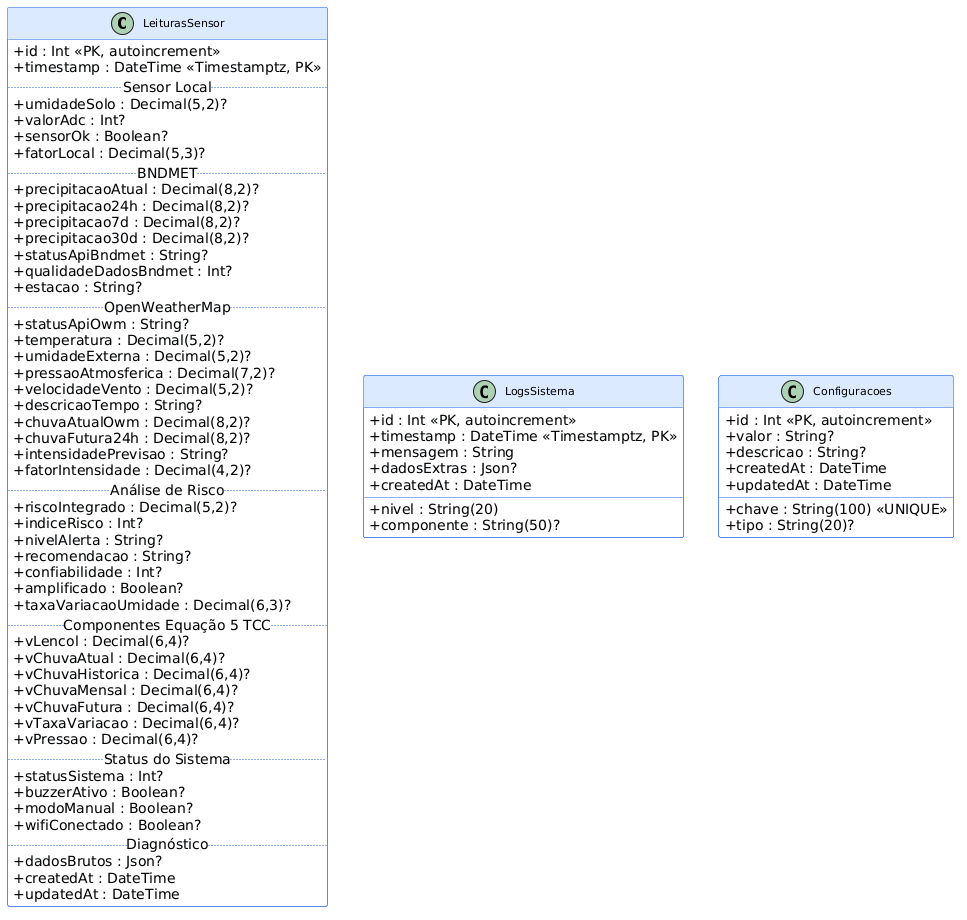
\includegraphics[width=\textwidth]{figures/image54_diagrama_classes_parte1.png}
  \caption{Diagrama de Classes — Parte 1: Modelos de Dados}
  \label{fig:diagrama_classes_parte1}
  \fonte{Autora, 2025.}
\end{figure}

A classe central é \texttt{LeiturasSensor}, que concentra todos os dados produzidos
por um ciclo completo de coleta e análise. Sua chave primária composta por
\texttt{id} e \texttt{timestamp} habilita o particionamento automático por tempo
do TimescaleDB, conferindo desempenho superior em consultas de séries temporais
\cite{timescaledb2024}. Os atributos estão organizados em seis grupos: dados do
sensor local (umidade, ADC, fator do lençol freático), precipitações BNDMET
(acumulados em 24h, 7d e 30d), dados OWM (temperatura, pressão, vento e previsão),
resultado da análise de risco (fator integrado, índice percentual e nível de alerta),
componentes individuais da equação de risco ($V_{len}$ a $V_{press}$) e diagnóstico
do firmware no campo \texttt{dadosBrutos} (\texttt{jsonb}), que contém descontos
de confiabilidade, sinalizadores de estado de ruptura e métricas de hardware.

A classe \texttt{LogsSistema} registra eventos operacionais do sistema classificados
por nível de criticidade (\texttt{INFO}, \texttt{WARNING}, \texttt{ERROR},
\texttt{CRITICAL}) e por componente de origem (\texttt{SENSOR}, \texttt{BNDMET},
\texttt{CONECTIVIDADE}). Assim como \texttt{LeiturasSensor}, sua chave primária é
composta pelo par \texttt{(id, timestamp)}, habilitando o mesmo mecanismo de
particionamento temporal do TimescaleDB. A classe \texttt{Configuracoes} armazena
parâmetros de configuração do sistema em formato chave–valor, permitindo ajustes
operacionais sem necessidade de recompilação do código.

% ─────────────────────────────────────────────────────────────
\subsubsubsection{Parte 2 — Modelos de Autenticação e Usuários}
% ─────────────────────────────────────────────────────────────

A Figura~\ref{fig:diagrama_classes_parte2} apresenta o modelo de dados responsável
pelo controle de acesso, gestão de usuários e registro de alertas enviados pelo
sistema.

\begin{figure}[H]
  \centering
  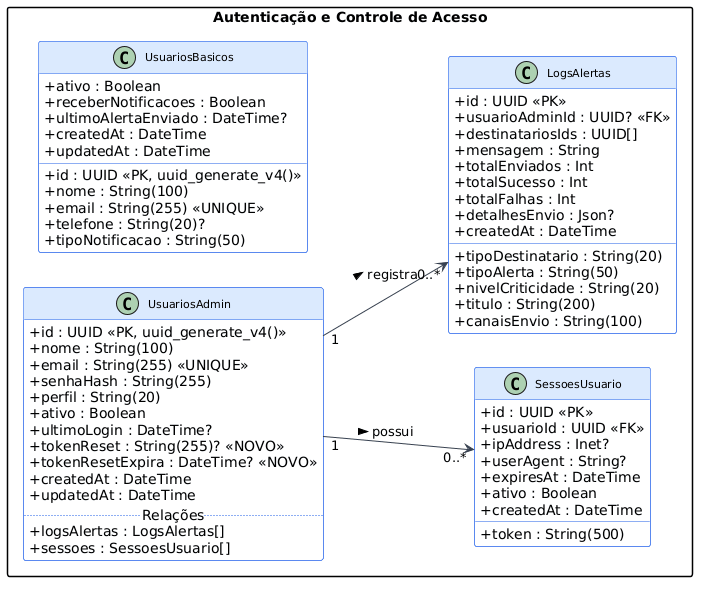
\includegraphics[width=\textwidth]{figures/image54_diagrama_classes_parte2.png}
  \caption{Diagrama de Classes — Parte 2: Autenticação e Usuários}
  \label{fig:diagrama_classes_parte2}
  \fonte{Autora, 2025.}
\end{figure}

A classe \texttt{UsuariosAdmin} representa os administradores, os únicos usuários com
capacidade de autenticação na interface \textit{web}. Seus identificadores são
UUIDs gerados pelo PostgreSQL e a senha é armazenada exclusivamente como
\textit{hash} via \texttt{bcryptjs}. Os campos \texttt{tokenReset} (token
hexadecimal de 64 caracteres) e \texttt{tokenResetExpira} (validade de duas
horas) suportam a recuperação de senha: são preenchidos na solicitação e
atribuídos a \texttt{null} após uso bem-sucedido, garantindo uso único.

A classe \texttt{UsuariosBasicos} representa os destinatários dos alertas do sistema,
como operadores de campo, engenheiros responsáveis e gestores que devem ser
notificados em situações de risco. Diferentemente dos administradores, esses usuários
não se autenticam no sistema, mas recebem alertas por e-mail ou SMS conforme
configurado nos campos \texttt{receberNotificacoes} e \texttt{tipoNotificacao}.

A classe \texttt{SessoesUsuario} implementa o controle de sessões JWT (\textit{JSON
Web Token}) de forma persistente no banco de dados, permitindo logout explícito e
a identificação de sessões ativas por endereço IP e agente de usuário. O campo
\texttt{ipAddress} utiliza o tipo nativo \texttt{Inet} do PostgreSQL para armazenar
endereços IPv4 e IPv6. Por fim, a classe \texttt{LogsAlertas} registra o histórico
completo de cada disparo de alerta em massa realizado pela Central de Alertas, incluindo
o número de destinatários, os resultados individuais de envio e o nível de criticidade
da mensagem.

% ─────────────────────────────────────────────────────────────
\subsubsubsection{Parte 3 — Camada de Serviços e Controladores}
% ─────────────────────────────────────────────────────────────

A Figura~\ref{fig:diagrama_classes_parte3} apresenta as classes da camada de negócio
e da camada de controle HTTP do \textit{backend} desenvolvido em Node.js com
TypeScript.

\begin{figure}[H]
  \centering
  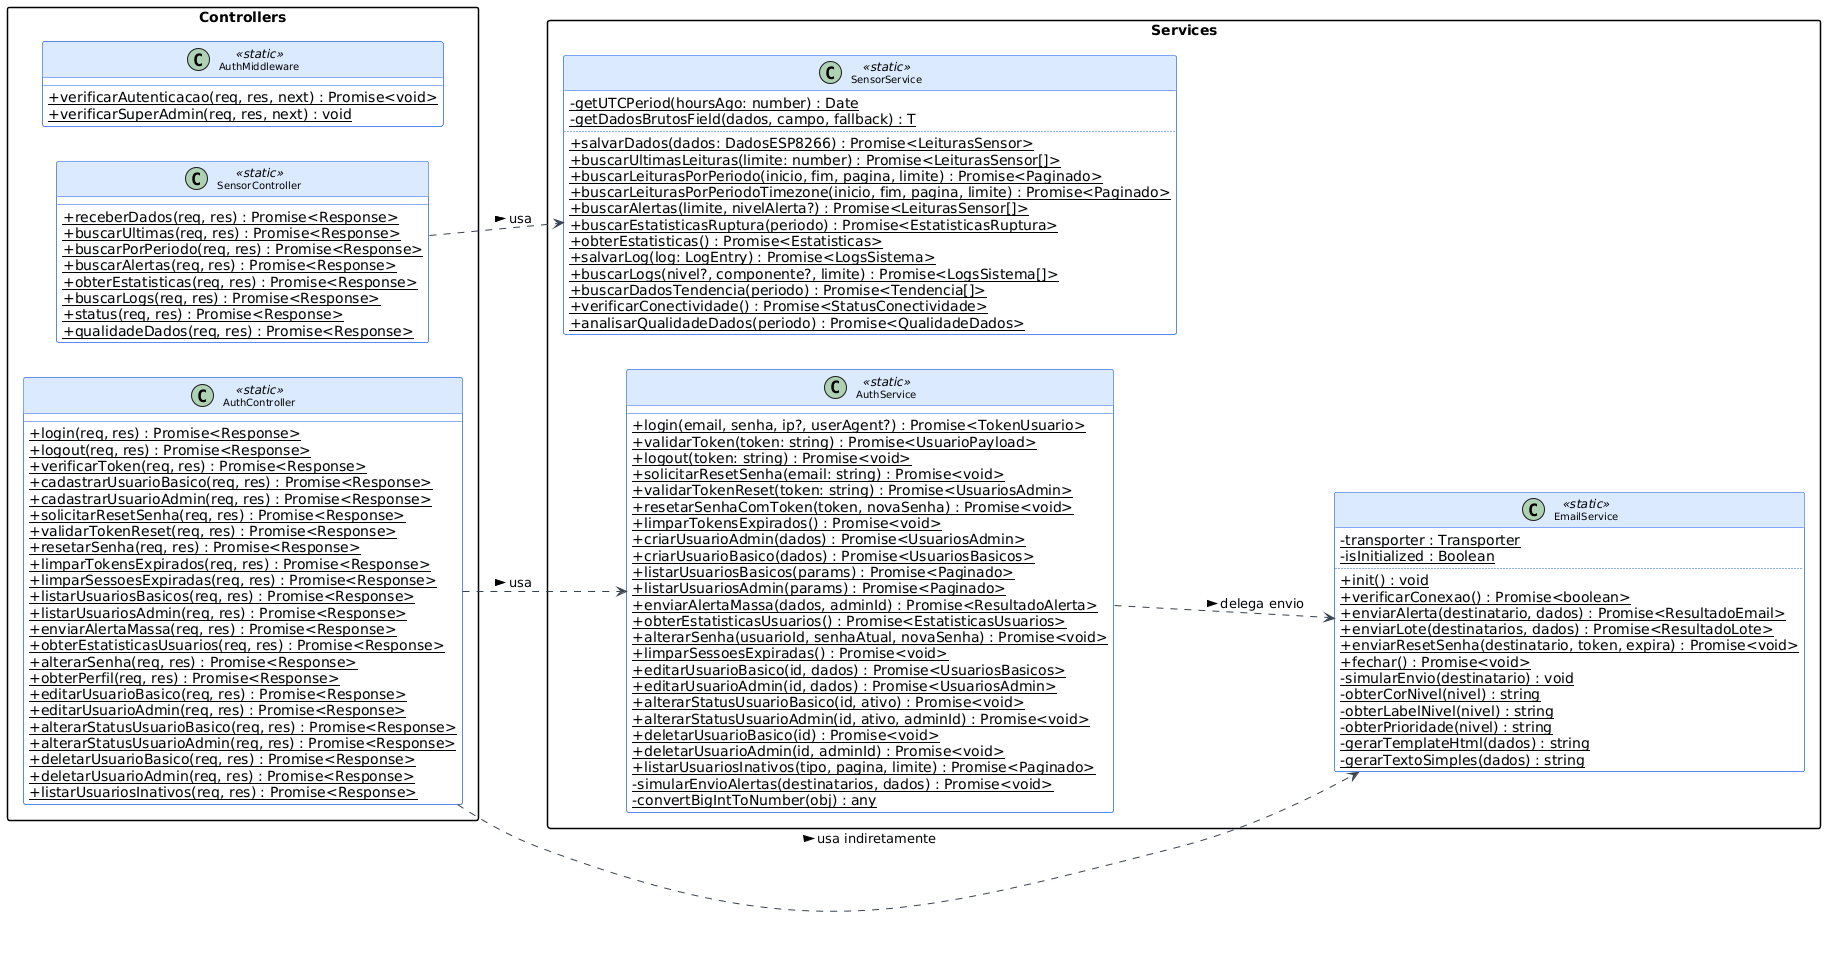
\includegraphics[width=\textwidth]{figures/image54_diagrama_classes_parte3.png}
  \caption{Diagrama de Classes — Parte 3: Serviços e Controladores}
  \label{fig:diagrama_classes_parte3}
  \fonte{Autora, 2025.}
\end{figure}

A arquitetura do \textit{backend} segue o padrão MVC (\textit{Model-View-Controller}),
separando as responsabilidades em camadas bem definidas. Todos os serviços e
controladores são implementados como classes com métodos estáticos (\textit{static}),
dispensando instanciação e tornando seu uso direto por referência à classe.

A classe \texttt{SensorService} concentra toda a lógica de negócio relacionada às
leituras do sensor. O método \texttt{salvarDados()} persiste no banco a leitura
completa recebida do ESP8266 via requisição HTTP POST, incluindo o tratamento
de campo booleano que corrige um bug identificado na versão anterior do firmware
— quando o sensor estava desconectado, o campo \texttt{sensorOk} chegava como
\texttt{undefined} e era gravado como \texttt{NULL} em vez de \texttt{false}.
O método \texttt{buscarEstatisticasRuptura()} foi introduzido para fornecer ao
\textit{frontend} informações agregadas sobre eventos de ruptura, como quantidade
de ocorrências, duração média e estado atual do sistema. Os métodos
\texttt{verificarConectividade()} e \texttt{analisarQualidadeDados()} expõem
campos específicos do firmware v13, como \texttt{bndmet\_inicializado} e
\texttt{aguardando\_reset\_ruptura}, possibilitando que o painel \textit{web}
apresente mensagens contextualizadas ao operador.

A classe \texttt{AuthService} gerencia toda a lógica de autenticação e autorização
do sistema. Além dos métodos tradicionais de \textit{login}, \textit{logout} e
gerenciamento de usuários, foram adicionados nesta versão três métodos específicos
para o fluxo de recuperação de senha: \texttt{solicitarResetSenha()}, responsável
por gerar o token, persistir no banco e acionar o envio do e-mail;
\texttt{validarTokenReset()}, que verifica a existência e a validade temporal do
token; e \texttt{resetarSenhaComToken()}, que atualiza o \textit{hash} da senha
e limpa os campos de token do banco de dados após uso bem-sucedido.

A classe \texttt{EmailService} gerencia o serviço de envio de e-mails utilizando a
biblioteca \texttt{nodemailer} configurada com servidor SMTP do Gmail. O método
\texttt{enviarAlerta()} é responsável pelo envio individual de notificações de risco
para destinatários cadastrados, enquanto \texttt{enviarLote()} processa o envio em
massa com controle de concorrência e \textit{retry}. O método
\texttt{enviarResetSenha()}, adicionado nesta versão, envia ao usuário um e-mail com
\textit{template} HTML contendo o token de recuperação em destaque e instruções
passo a passo para redefinição da senha, com \textit{fallback} em texto simples para
clientes de e-mail que não suportam HTML.

Os controladores \texttt{SensorController} e \texttt{AuthController} atuam como
intermediários entre as rotas HTTP e os serviços de negócio, sendo responsáveis
exclusivamente por receber as requisições, validar os dados de entrada, delegar o
processamento aos serviços e formatar as respostas padronizadas. A classe
\texttt{AuthMiddleware} implementa o mecanismo de proteção das rotas, verificando a
validade do token JWT em cada requisição às rotas autenticadas e controlando o acesso
a funcionalidades restritas a administradores com perfil \texttt{superadmin}.

% ─────────────────────────────────────────────────────────────
\subsubsubsection{Parte 4 — Sistema Embarcado}
% ─────────────────────────────────────────────────────────────

A Figura~\ref{fig:diagrama_classes_parte4} apresenta as estruturas de dados e as
funções do firmware embarcado no microcontrolador ESP8266 NodeMCU, implementado
em linguagem C++ para o ambiente Arduino.

\begin{figure}[H]
  \centering
  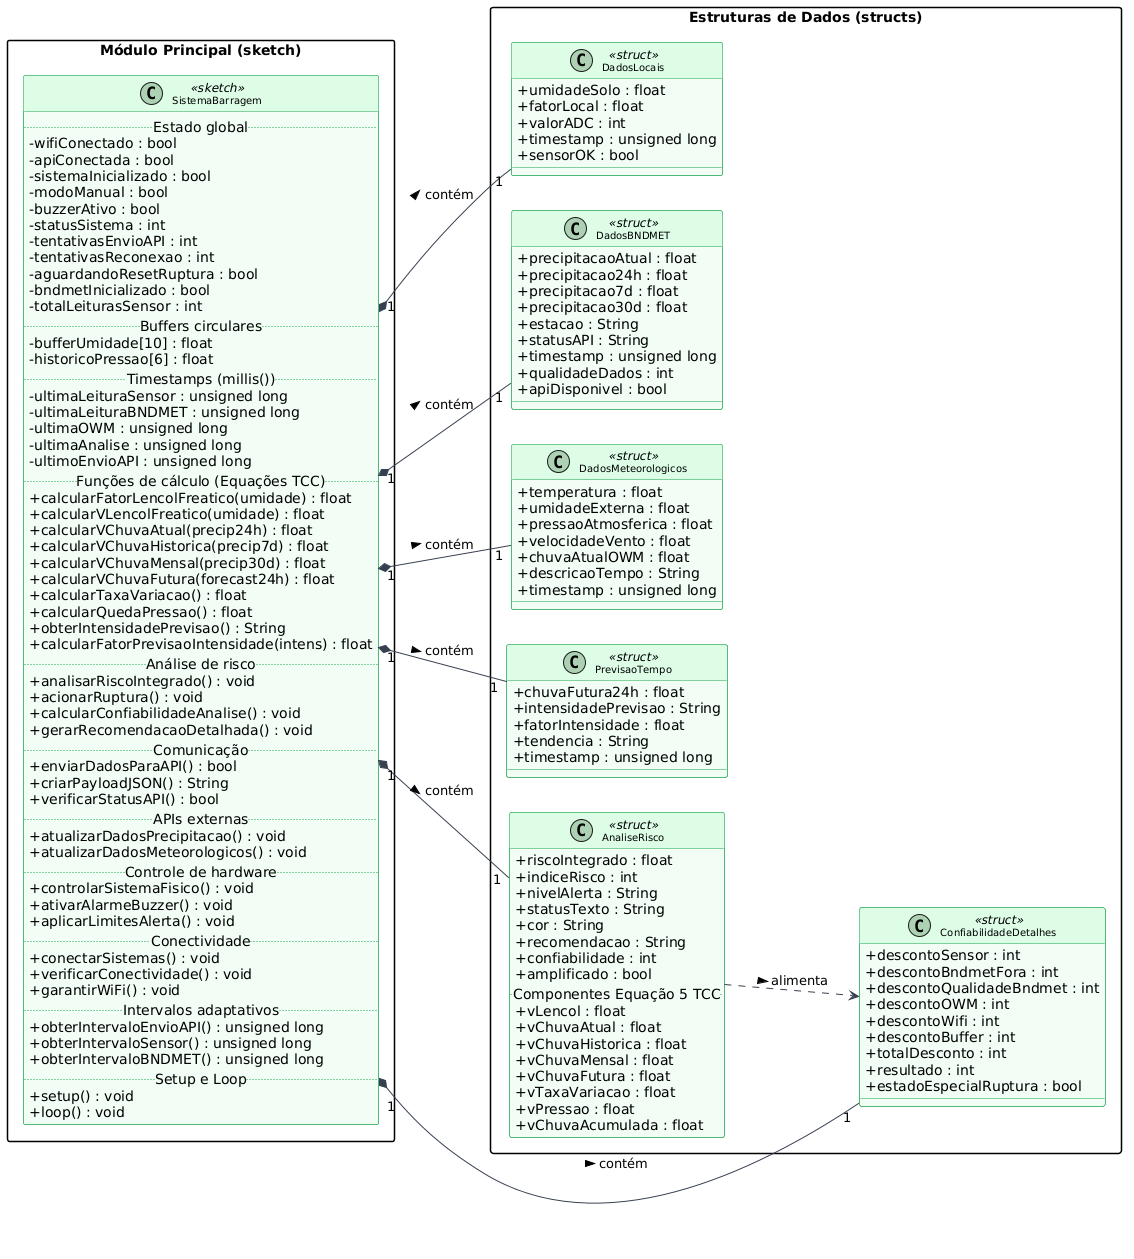
\includegraphics[width=\textwidth]{figures/image54_diagrama_classes_parte4.png}
  \caption{Diagrama de Classes — Parte 4: Sistema Embarcado (ESP8266)}
  \label{fig:diagrama_classes_parte4}
  \fonte{Autora, 2025.}
\end{figure}

O firmware não adota o paradigma de orientação a objetos com classes formais
instanciáveis, padrão do ambiente Arduino em C++. A encapsulação é realizada por
meio de estruturas (\textit{structs}), variáveis globais e funções, organizadas de
forma coesa por domínio funcional. Para fins de representação no diagrama, as
estruturas são modeladas como classes com o estereótipo \texttt{<<struct>>} e as
funções globais são agrupadas na classe representativa \texttt{SistemaBarragem}
com o estereótipo \texttt{<<sketch>>}, seguindo convenção adotada em trabalhos
similares \cite{guedes2011uml}.

A estrutura \texttt{DadosLocais} agrupa as informações coletadas diretamente pelo
higrômetro capacitivo conectado ao pino analógico A0: a umidade do solo em
percentual, o valor ADC bruto (inteiro entre 0 e 1023), o fator do lençol freático
normalizado ($F_{len\c{c}ol} = umidade / UMIDADE\_CRITICA$, conforme Equação~3 do
TCC) e uma \textit{flag} indicando se o sensor está operacional. A estrutura
\texttt{DadosBNDMET} armazena as precipitações pluviométricas obtidas da API
BNDMET/DECEA para a estação D6594 (Alberto Flores, ANA): acumulados em 24 horas,
7 dias e 30 dias, além do status da última requisição e do percentual de qualidade
dos dados retornados. A estrutura \texttt{DadosMeteorologicos} consolida os dados
meteorológicos atuais provenientes da API OpenWeatherMap: temperatura,
umidade relativa do ar, pressão atmosférica, velocidade do vento, precipitação atual
e descrição textual das condições. A estrutura \texttt{PrevisaoTempo} armazena a
precipitação total prevista para as próximas 24 horas, obtida a partir da soma dos
blocos de previsão do endpoint \texttt{/forecast} da mesma API.

A estrutura \texttt{AnaliseRisco} é a mais complexa do firmware e representa o
resultado completo do cálculo da Equação~5 do TCC. Além do fator de risco integrado
e do nível de alerta, ela armazena os sete componentes individuais da equação já
com seus respectivos pesos aplicados: $V_{len\c{c}ol}$ (peso 0,40),
$V_{ch.atual}$ (peso 0,08), $V_{ch.hist.}$ (peso 0,12), $V_{ch.mensal}$
(peso 0,10), $V_{ch.fut.}$ (peso 0,15), $V_{taxa}$ (peso 0,10) e
$V_{press\~ao}$ (peso 0,05), totalizando soma de pesos igual a 1,00. Esses
componentes são serializados no \textit{payload} JSON enviado ao \textit{backend}
e persistidos individualmente no banco de dados, permitindo auditoria detalhada
de cada ciclo de análise.

A estrutura \texttt{ConfiabilidadeDetalhes} registra os descontos aplicados no cálculo
do índice de confiabilidade da análise, conforme tabela de pesos documentada no
capítulo de metodologia: falha do sensor físico ($-40\%$), API BNDMET indisponível
($-25\%$), qualidade BNDMET inferior a 80\% ($-10\%$), API OWM indisponível
($-15\%$), WiFi desconectado ($-10\%$) e buffer histórico insuficiente ($-10\%$).
No estado especial de ruptura, a confiabilidade é fixada em 100\%
independentemente dos descontos, pois o hardware confirma diretamente o estado
crítico. Os detalhes desta estrutura são serializados dentro do campo
\texttt{dadosBrutos} de cada registro no banco de dados, tornando auditável cada
decisão de confiabilidade pelo painel \textit{web}.

A classe \texttt{SistemaBarragem} agrupa as funções globais do \textit{sketch} em
grupos funcionais: funções de cálculo das equações do TCC, funções de análise de
risco (incluindo o tratamento de ruptura e o cálculo de confiabilidade), funções de
comunicação HTTP com o \textit{backend} e com as APIs externas, funções de controle
de hardware (LEDs, buzzer) e funções de conectividade WiFi. O ciclo de operação é
controlado pela função \texttt{loop()}, que verifica temporizadores individuais para
cada subsistema — leitura de sensor, consulta BNDMET, consulta OWM, análise de risco
e envio para o \textit{backend} — e aciona cada um no intervalo adequado ao nível de
alerta vigente. Os intervalos são adaptativos em todos os subsistemas: a leitura do
higrômetro ocorre a cada 30 segundos no nível VERDE, 10 segundos no nível AMARELO
e 5 segundos no nível VERMELHO; a consulta à API BNDMET ocorre a cada 5 minutos no
nível VERDE, 2 minutos no nível AMARELO e 1 minuto no nível VERMELHO; o envio ao
\textit{backend} ocorre a cada 60 segundos no nível VERDE, 20 segundos no nível
AMARELO e 10 segundos no nível VERMELHO. As consultas à OpenWeatherMap seguem
timers fixos independentes do nível de alerta: \texttt{/weather} a cada 10 minutos e
\texttt{/forecast} a cada 30 minutos. Essa granularidade diferenciada por subsistema
permite que o sistema intensifique simultaneamente a aquisição local, a atualização
meteorológica e a comunicação com o \textit{backend} nos cenários de maior criticidade.

% -------------------------------------------------------------
\subsubsection{Diagramas de Sequência}
\label{subsubsec:sequencia}

O diagrama de sequência é um dos diagramas comportamentais da UML e tem por
finalidade representar a troca de mensagens entre os objetos de um sistema ao longo
do tempo, evidenciando a ordem cronológica das interações e os atores envolvidos em
cada fluxo \cite{guedes2011uml}. Diferentemente do diagrama de classes, que descreve
a estrutura estática do sistema, o diagrama de sequência descreve o comportamento
dinâmico, sendo especialmente útil para detalhar como as camadas da arquitetura
colaboram para produzir um resultado.

Dado o escopo do sistema desenvolvido — que integra hardware embarcado, APIs
externas, banco de dados e interface \textit{web} — o conjunto de interações é extenso
e variado. Para garantir legibilidade e facilitar a compreensão de cada fluxo, o diagrama
foi organizado em sete grupos lógicos, cada um subdividido em partes que cobrem um
bloco de interação específico: (1) inicialização do ESP8266; (2) ciclo de coleta e envio
de dados; (3) autenticação do administrador; (4) recuperação de senha; (5) monitoramento
via \textit{dashboard}; (6) tela de sensores, filtros e relatórios; e (7) gestão de
usuários e central de alertas.

% ─────────────────────────────────────────────────────────────
\subsubsubsection{Parte 1 — Boot e Inicialização do ESP8266}
% ─────────────────────────────────────────────────────────────

O processo de inicialização do ESP8266 ocorre automaticamente ao energizar o
dispositivo, seja por conexão USB ou por fonte de alimentação independente na tomada,
e é executado integralmente pela função \texttt{setup()}, única no ambiente Arduino.

A Figura~\ref{fig:seq_1a} apresenta a inicialização de hardware. A primeira ação do
\texttt{setup()} é a leitura da calibração persistida na EEPROM: se os valores de
\texttt{SENSOR\_SECO} e \texttt{SENSOR\_UMIDO} gravados nos endereços 0 e 4 forem
válidos (entre 0 e 1023), eles substituem os padrões de fábrica, preservando a
calibração entre reinicializações. Em seguida, os pinos GPIO dos LEDs e do buzzer são
configurados e uma sequência de teste visual é executada: os três LEDs acendem em
ordem (verde, amarelo, vermelho, 400 ms cada) e o buzzer emite um sinal breve,
confirmando ao operador que os periféricos estão operacionais antes de qualquer
comunicação de rede.

\begin{figure}[H]
  \centering
  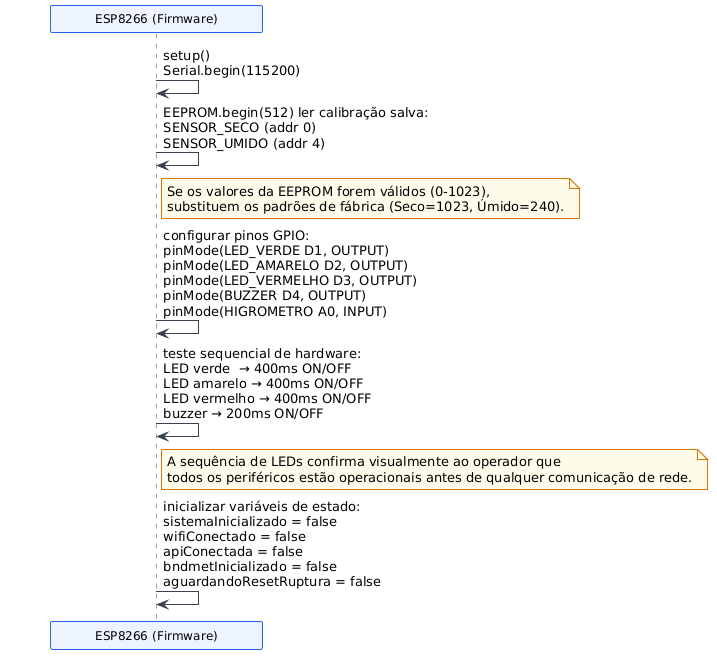
\includegraphics[width=0.85\textwidth]{figures/image55_seq_1a.png}
  \caption{Seq. 1a — Inicialização de Hardware (ESP8266)}
  \label{fig:seq_1a}
  \fonte{Autora, 2025.}
\end{figure}

A Figura~\ref{fig:seq_1b} ilustra a conexão Wi-Fi. O firmware configura o modo
\texttt{WIFI\_STA} e tenta conectar-se à rede definida em tempo de compilação,
verificando o status a cada 1.000 milissegundos por no máximo 20 tentativas (20
segundos). Ao obter o endereço IP via DHCP, \texttt{wifiConectado} é definido como
\texttt{true} e o cliente seguro \texttt{wifiClientSecure.setInsecure()} é inicializado
para as comunicações HTTPS com as APIs externas. Caso o tempo esgote, o
\texttt{setup()} prossegue sem conectividade, operando localmente até que a
reconexão ocorra em ciclo posterior.

\begin{figure}[H]
  \centering
  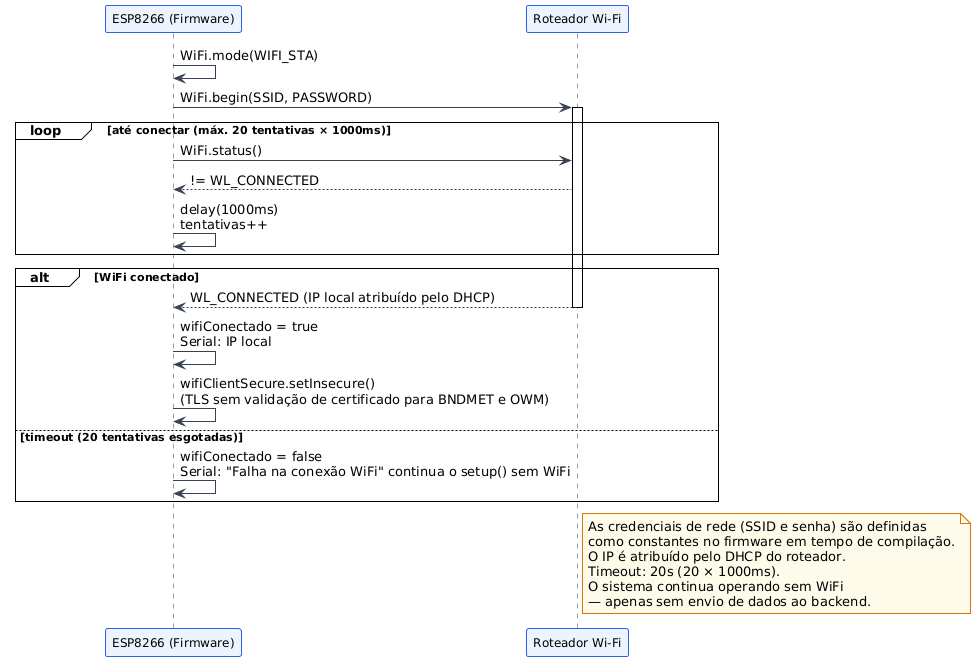
\includegraphics[width=0.85\textwidth]{figures/image55_seq_1b.png}
  \caption{Seq. 1b — Conexão Wi-Fi}
  \label{fig:seq_1b}
  \fonte{Autora, 2025.}
\end{figure}

A Figura~\ref{fig:seq_1c} mostra a sincronização com o servidor NTP
(\textit{Network Time Protocol}), realizada com \texttt{configTime(-3×3600, 0,
"pool.ntp.org", "time.nist.gov")} para o fuso horário de Brasília (UTC$-$3). O
firmware aguarda até 20 iterações de 500 milissegundos (10 segundos no total) por um
\textit{timestamp} Unix superior a 1.000.000.000, que corresponde a uma data
posterior a 2001. Caso o tempo esgote, o \texttt{setup()} continua sem horário
válido — comportamento gracioso que evita travamento do dispositivo. O campo
\texttt{bndmetInicializado} permanece \texttt{false} enquanto o NTP não for
sincronizado, impedindo que consultas à API BNDMET com datas inválidas (1969-12-31)
contaminem as métricas de qualidade dos dados pluviométricos no banco de dados.

\begin{figure}[H]
  \centering
  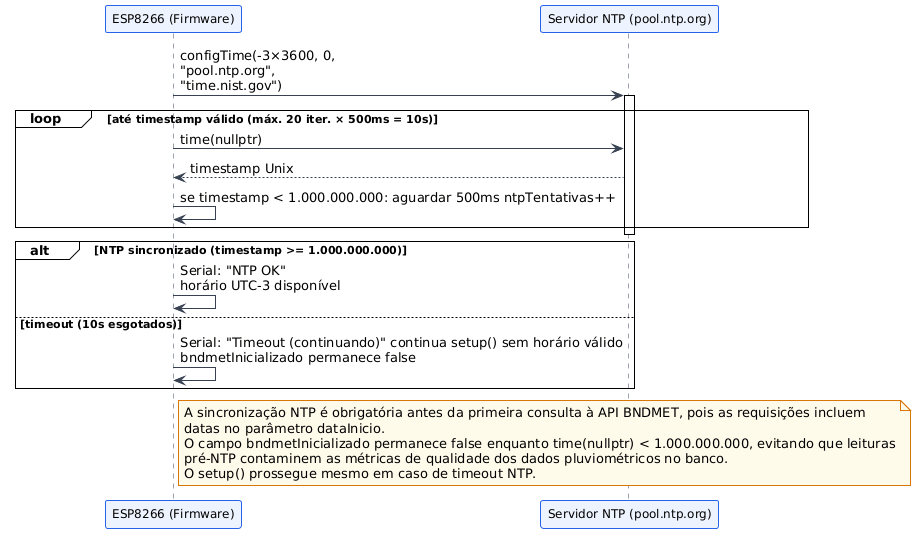
\includegraphics[width=0.85\textwidth]{figures/image55_seq_1c.png}
  \caption{Seq. 1c — Sincronização NTP}
  \label{fig:seq_1c}
  \fonte{Autora, 2025.}
\end{figure}

A Figura~\ref{fig:seq_1d} apresenta a verificação do \textit{backend} local. O
firmware consulta o endpoint \texttt{GET /api/sensor/status} — via HTTP simples sem TLS, pois ESP8266 e servidor encontram-se
na mesma rede local. A comunicação com as APIs externas BNDMET e OpenWeatherMap
utiliza HTTPS com TLS via \texttt{WiFiClientSecure}. Um \textit{timeout} de 5.000
milissegundos é configurado para a requisição; em caso de falha, o sistema continua
sem \textit{backend}.

\begin{figure}[H]
  \centering
  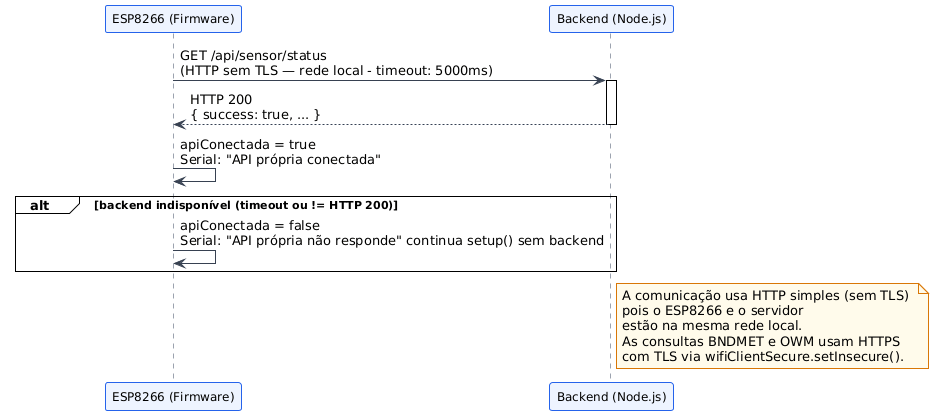
\includegraphics[width=0.85\textwidth]{figures/image55_seq_1d.png}
  \caption{Seq. 1d — Verificação do Backend}
  \label{fig:seq_1d}
  \fonte{Autora, 2025.}
\end{figure}

Por fim, a Figura~\ref{fig:seq_1e} apresenta a primeira coleta completa de dados.
Após a leitura do sensor local, o firmware verifica imediatamente se a umidade já
atingiu o limiar de ruptura de 30\%: em caso positivo, \texttt{acionarRuptura()} é
chamada e as consultas às APIs externas são suprimidas. No fluxo normal, BNDMET e
OpenWeatherMap são consultados com um \textit{delay} de 1.000 milissegundos entre
cada requisição, seguidos da análise de risco e do envio inicial ao \textit{backend}.
Ao final, os \textit{timestamps} de controle são inicializados e \texttt{sistemaInicializado}
é definido como \texttt{true}. O sistema entra então no ciclo autônomo da função
\texttt{loop()} com intervalos adaptativos de produção: leitura do sensor a cada 30 s
(VERDE), 10 s (AMARELO) ou 5 s (VERMELHO); envio ao \textit{backend} a cada 60 s,
20 s ou 10 s respectivamente; BNDMET a cada 5 min, 2 min ou 1 min; e OpenWeatherMap
a cada 30 min. O modo de teste com envio fixo a cada 10 s, disponível na versão 15
do firmware, está comentado na versão 16 em uso.

\begin{figure}[H]
  \centering
  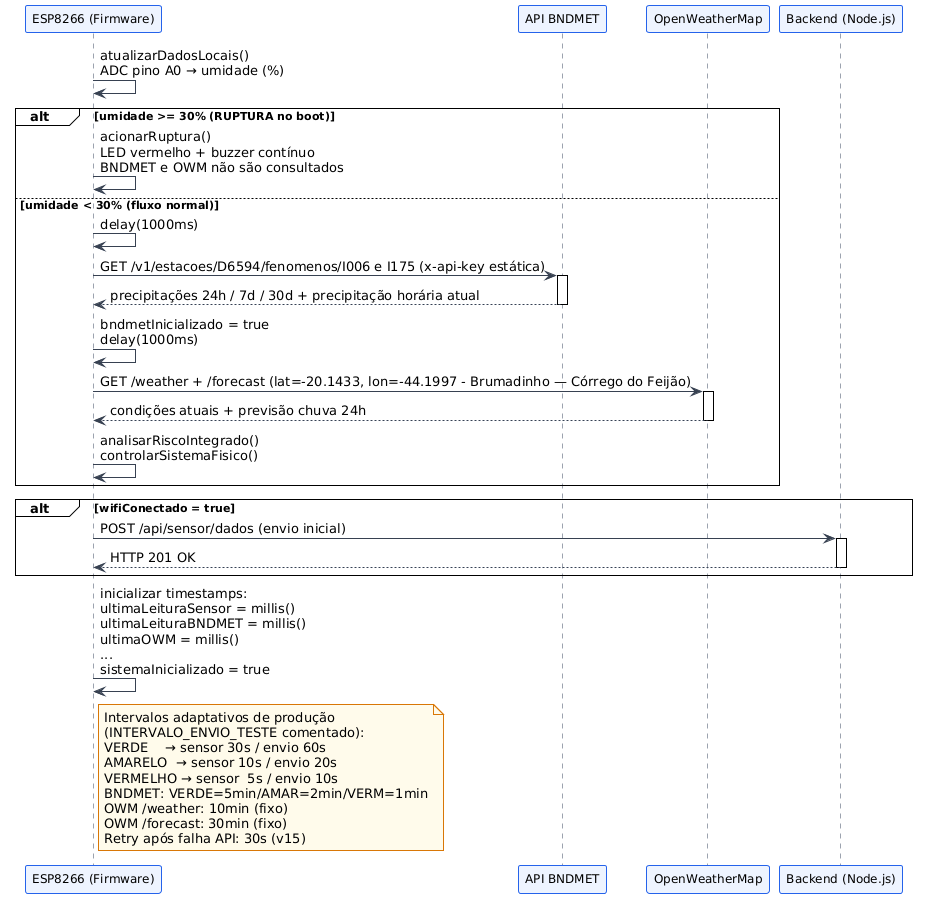
\includegraphics[width=0.85\textwidth]{figures/image55_seq_1e.png}
  \caption{Seq. 1e — Primeira Coleta Inicial}
  \label{fig:seq_1e}
  \fonte{Autora, 2025.}
\end{figure}

% ─────────────────────────────────────────────────────────────
\subsubsubsection{Parte 2 — Ciclo de Coleta, Análise de Risco e Envio}
% ─────────────────────────────────────────────────────────────

O ciclo principal de operação autônoma é executado continuamente pela função
\texttt{loop()}, com temporizadores individuais controlando o intervalo de cada
subsistema de forma independente.

A Figura~\ref{fig:seq_2a} detalha a leitura do sensor local. O valor ADC do pino A0
(0–1023) é mapeado para percentual de umidade do solo e o fator do lençol freático
normalizado é calculado como $F_{len\c{c}ol} = \text{constrain}(\text{umidade} / 25\%,
0, 1)$, conforme a Equação~3 do TCC. A variável \texttt{sensorOK} é definida como
\texttt{false} quando o ADC é igual a 0 (curto-circuito) ou igual a 1023 (circuito
aberto, sensor desconectado), aplicando desconto de $-40\%$ na confiabilidade. O
buffer circular de 10 posições é atualizado a cada leitura para o cálculo posterior da
taxa de variação de umidade, e o contador não-circular \texttt{totalLeiturasSensor}
é incrementado — este último é utilizado para aplicar desconto de $-10\%$ na
confiabilidade quando inferior a 5, indicando buffer histórico insuficiente.

\begin{figure}[H]
  \centering
  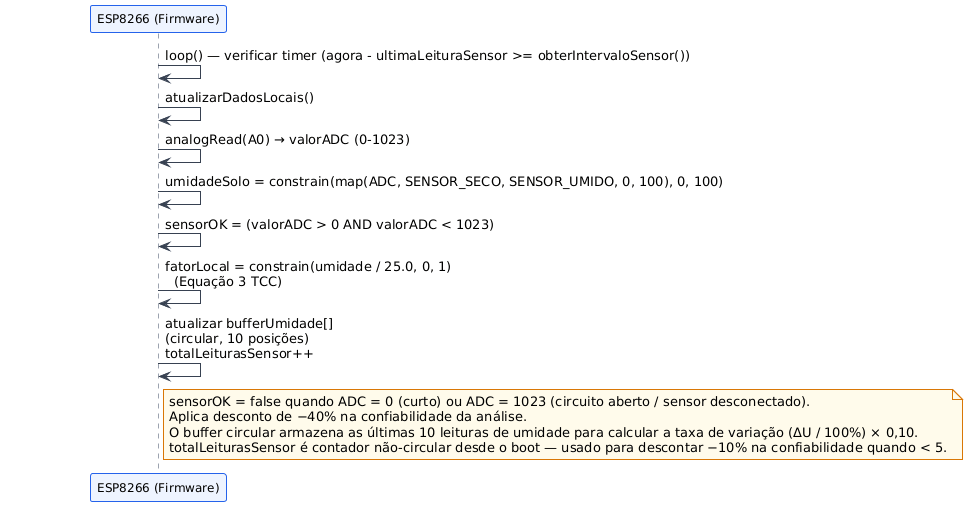
\includegraphics[width=0.85\textwidth]{figures/image55_seq_2a.png}
  \caption{Seq. 2a — Leitura do Sensor Local}
  \label{fig:seq_2a}
  \fonte{Autora, 2025.}
\end{figure}

A Figura~\ref{fig:seq_2b} ilustra a consulta à API BNDMET/DECEA para a estação D6594
(Alberto Flores, ANA). Um mecanismo de \textit{retry} acelerado introduzido na versão
15 do firmware reduz o intervalo de consulta para 30 segundos quando
\texttt{apiDisponivel = false}, acelerando a recuperação após falhas temporárias da API
sem aguardar o intervalo normal de 5 minutos. Adicionalmente, uma guarda NTP
implementada na versão 13 impede que a consulta seja realizada quando
\texttt{time(nullptr) < 1.000.000.000}, evitando requisições com datas inválidas. A
autenticação utiliza chave de API estática no cabeçalho \texttt{x-api-key}, o que
garante a autonomia do firmware sem necessidade de renovação de credenciais —
característica fundamental para operação embarcada, incompatível com o modelo de
\textit{tokens} de curta validade do HidroWeb.

\begin{figure}[H]
  \centering
  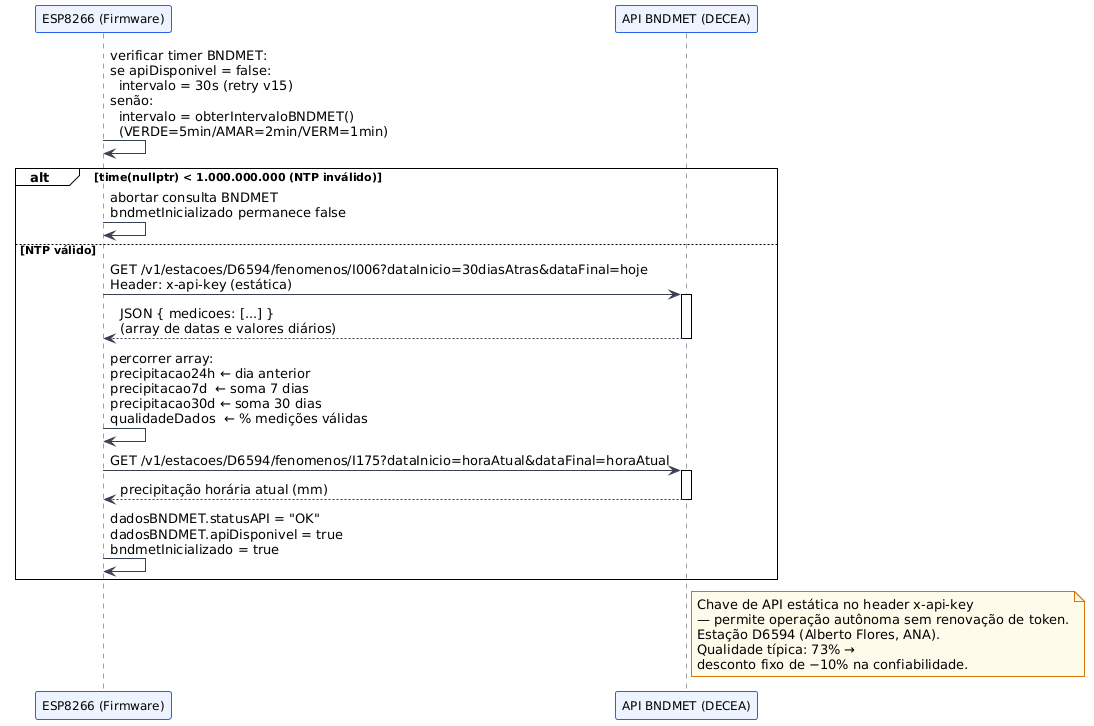
\includegraphics[width=0.85\textwidth]{figures/image55_seq_2b.png}
  \caption{Seq. 2b — Consulta BNDMET}
  \label{fig:seq_2b}
  \fonte{Autora, 2025.}
\end{figure}

A Figura~\ref{fig:seq_2c} apresenta as duas consultas ao OpenWeatherMap, realizadas
no servidor \texttt{pro.openweathermap.org} com as coordenadas de Brumadinho —
Córrego do Feijão ($\text{lat} = -20.1433$, $\text{lon} = -44.1997$). O endpoint
\texttt{/weather} fornece as condições meteorológicas atuais, e o endpoint
\texttt{/forecast} com \texttt{cnt=8} fornece os oito blocos de previsão de 3 horas,
cuja soma resulta na precipitação prevista para as próximas 24 horas. Assim como no
BNDMET, o mecanismo de \textit{retry} acelerado de 30 segundos é ativado quando
\texttt{dadosMeteo.timestamp = 0}, indicando que nenhuma consulta bem-sucedida
ocorreu ainda. A intensidade da previsão é classificada em cinco categorias conforme a
Tabela~4 do TCC: Fraca ($<5$ mm, fator 0,00), Moderada (5–25 mm, fator 0,25), Forte
(25–50 mm, fator 0,50), Muito Forte (50–80 mm, fator 0,75) e Pancada de Chuva
($\geq 80$ mm, fator 1,00).

\begin{figure}[H]
  \centering
  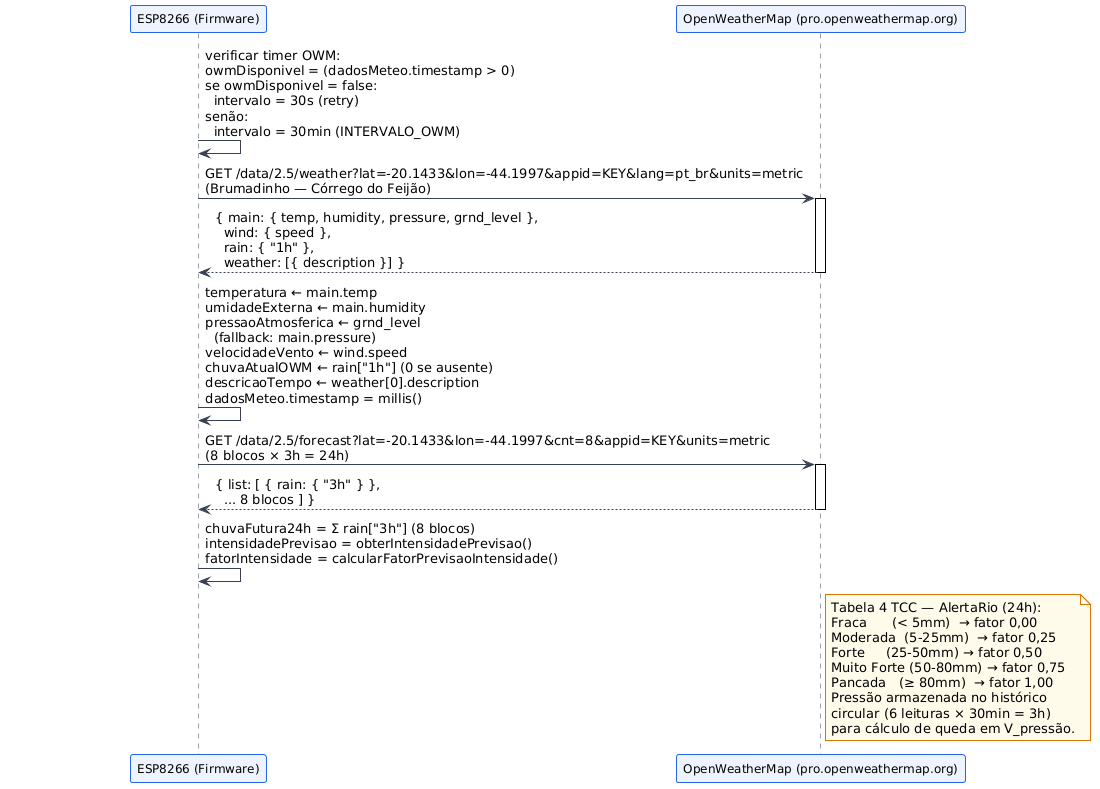
\includegraphics[width=0.85\textwidth]{figures/image55_seq_2c.png}
  \caption{Seq. 2c — Consulta OpenWeatherMap}
  \label{fig:seq_2c}
  \fonte{Autora, 2025.}
\end{figure}

A Figura~\ref{fig:seq_2d} detalha o cálculo da análise de risco pela Equação~5 do TCC.
Os sete componentes ponderados são calculados com \texttt{constrain} para limitar
cada contribuição ao intervalo $[0, 1]$ antes da multiplicação pelo peso. A taxa de
variação de umidade usa \texttt{fabsf()} para que tanto absorção quanto drenagem
rápida do solo contribuam ao risco, normalizando pela variação máxima de 100\%
(correção da versão 12, que substituiu a divisão por 10\%, a qual saturava o componente
em eventos extremos). Quando $F_{len\c{c}ol} \geq 0{,}70$ (equivalente a umidade $\geq 17{,}5\%$)
e a previsão é igual ou superior à classe Moderada ($\geq 5$ mm), um coeficiente de
amplificação de $\times 1{,}20$ é aplicado sobre a soma, sinalizando risco composto.
Quando a umidade do solo atinge 30\%, a função \texttt{acionarRuptura()} sobrepõe
o fator com o valor máximo de 1,0 e fixa a confiabilidade em 100\%, pois o hardware
confirma diretamente o estado crítico.

\begin{figure}[H]
  \centering
  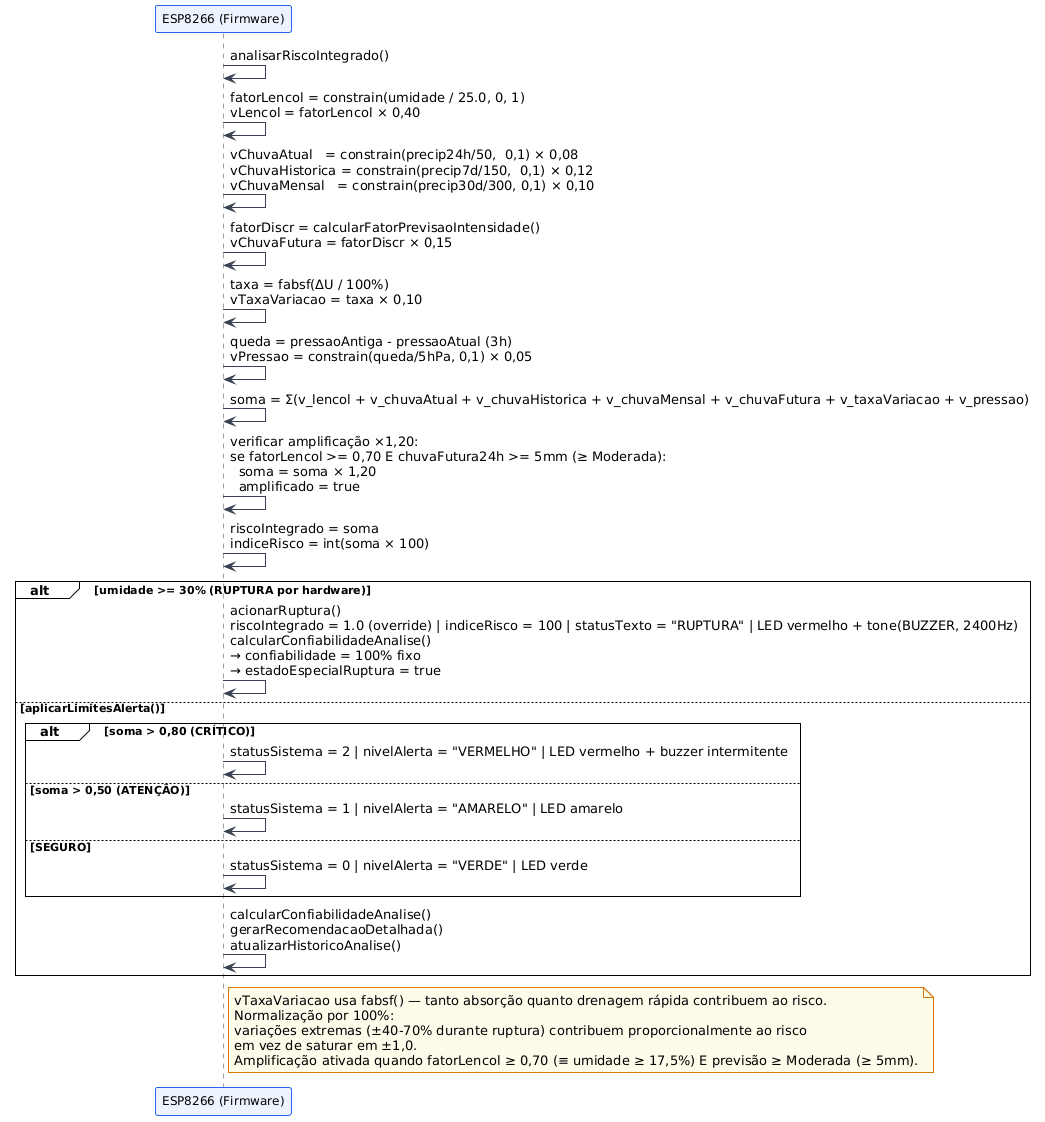
\includegraphics[width=0.85\textwidth]{figures/image55_seq_2d.png}
  \caption{Seq. 2d — Cálculo da Análise de Risco (Equação 5 TCC)}
  \label{fig:seq_2d}
  \fonte{Autora, 2025.}
\end{figure}

A Figura~\ref{fig:seq_2e} mostra o envio do \textit{payload} JSON ao \textit{backend}
via \texttt{POST /api/sensor/dados} com \textit{timeout} de 15.000 milissegundos. O
objeto contém aproximadamente 35 campos, incluindo o objeto \texttt{dadosBrutos} com
informações de diagnóstico do firmware (memória livre, RSSI, \textit{uptime},
tentativas de envio, sinalizador de \textit{cooldown} de ruptura, inicialização do
BNDMET e detalhamento dos descontos de confiabilidade por fonte). Os intervalos de
envio são adaptativos por nível de alerta — 60 s (VERDE), 20 s (AMARELO) e 10 s
(VERMELHO) — com o modo de teste de 10 s fixo disponível mas comentado na versão 16.
Em caso de falhas consecutivas, um \textit{watchdog} executa a cada 5 minutos e
reinicia o módulo Wi-Fi ou o dispositivo conforme a gravidade da situação.

\begin{figure}[H]
  \centering
  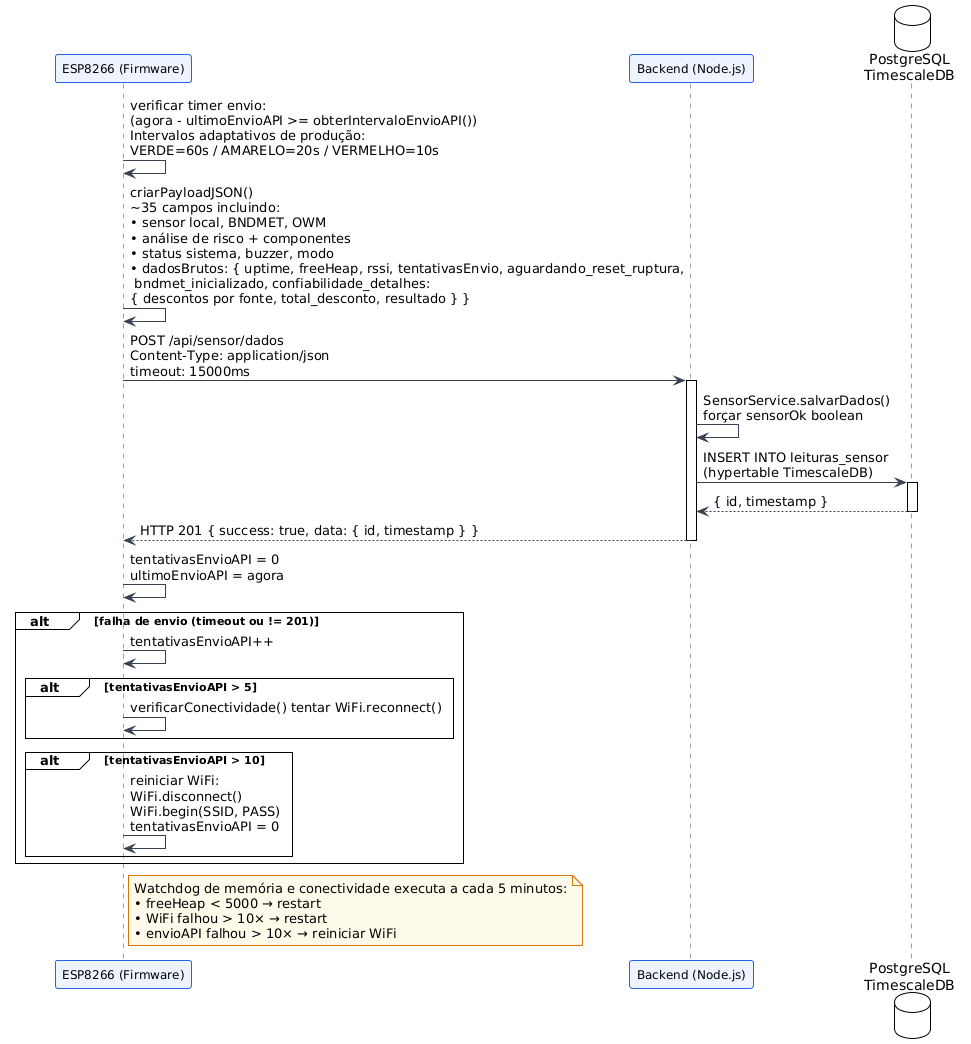
\includegraphics[width=0.85\textwidth]{figures/image55_seq_2e.png}
  \caption{Seq. 2e — Envio de Dados para o Backend}
  \label{fig:seq_2e}
  \fonte{Autora, 2025.}
\end{figure}

% ─────────────────────────────────────────────────────────────
\subsubsubsection{Parte 3 — Autenticação do Administrador}
% ─────────────────────────────────────────────────────────────

O módulo de autenticação é responsável por controlar o acesso à interface
\textit{web} de monitoramento, restrita exclusivamente aos administradores cadastrados.

A Figura~\ref{fig:seq_3a} apresenta o fluxo de \textit{login}. O frontend delega
a operação ao \texttt{AuthContext}, que chama \texttt{authService.login()} e
submete as credenciais ao endpoint \texttt{POST /auth/login}. O \textit{backend}
localiza o usuário pelo e-mail e valida a senha contra o \textit{hash} armazenado
utilizando a biblioteca \texttt{bcryptjs} com \textit{salt rounds} igual a 10.
Em caso de credenciais inválidas, a resposta HTTP 401 é propositalmente genérica —
sem indicar se o e-mail ou a senha está incorreto — como medida de segurança contra
ataques de enumeração de usuários \cite{owasp2021}. Quando as credenciais são
válidas, o \textit{backend} gera um token JWT com validade de 24 horas, persiste a
sessão na tabela \texttt{sessoes\_usuario} com o endereço IP e o agente de usuário,
e atualiza o campo \texttt{ultimoLogin} do administrador. A resposta HTTP 200 inclui
\texttt{token}, \texttt{usuario} e \texttt{expiresAt}. O \texttt{AuthContext} então
persiste o token e os dados do usuário em duas entradas separadas do
\texttt{localStorage} — \texttt{'token'} e \texttt{'user'} — e atualiza o estado
interno da aplicação.

\begin{figure}[H]
  \centering
  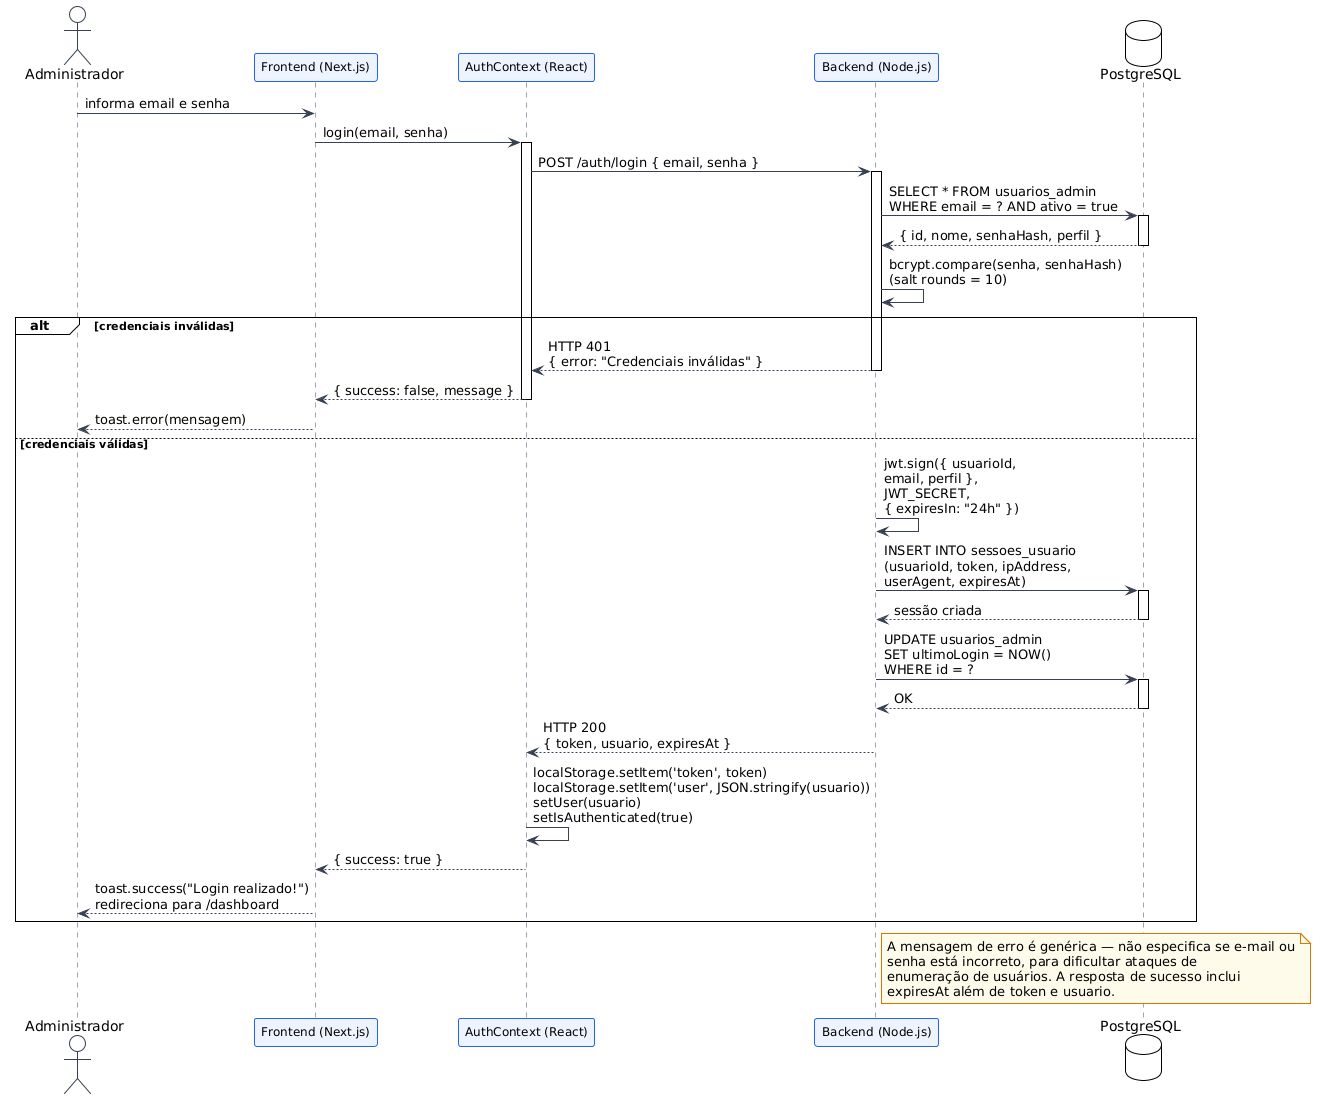
\includegraphics[width=0.85\textwidth]{figures/image55_seq_3a.png}
  \caption{Seq. 3a — Login do Administrador}
  \label{fig:seq_3a}
  \fonte{Autora, 2025.}
\end{figure}

A Figura~\ref{fig:seq_3b} ilustra a verificação de autenticidade nas rotas
protegidas. Diferentemente do que poderia sugerir uma leitura superficial,
não existe um endpoint específico chamado pelo \textit{frontend} para verificar
o token: o \texttt{AuthMiddleware} é um \textit{middleware} Express que intercepta
automaticamente todas as requisições às rotas decoradas com
\texttt{verificarAutenticacao}, sem ação explícita do cliente. O interceptor do
Axios, configurado em \texttt{api.js}, injeta o cabeçalho
\texttt{Authorization: Bearer <token>} em todas as requisições automaticamente,
lendo o token do \texttt{localStorage}. O \textit{middleware} extrai o token
do cabeçalho e chama \texttt{AuthService.validarToken()}, que realiza a verificação
da assinatura JWT seguida de uma consulta ao banco de dados confirmando que a sessão
está ativa e não expirou. Essa dupla verificação — assinatura criptográfica mais
estado persistido — é o que permite o logout explícito com invalidação imediata,
antes que o prazo natural de 24 horas do token se esgote.

\begin{figure}[H]
  \centering
  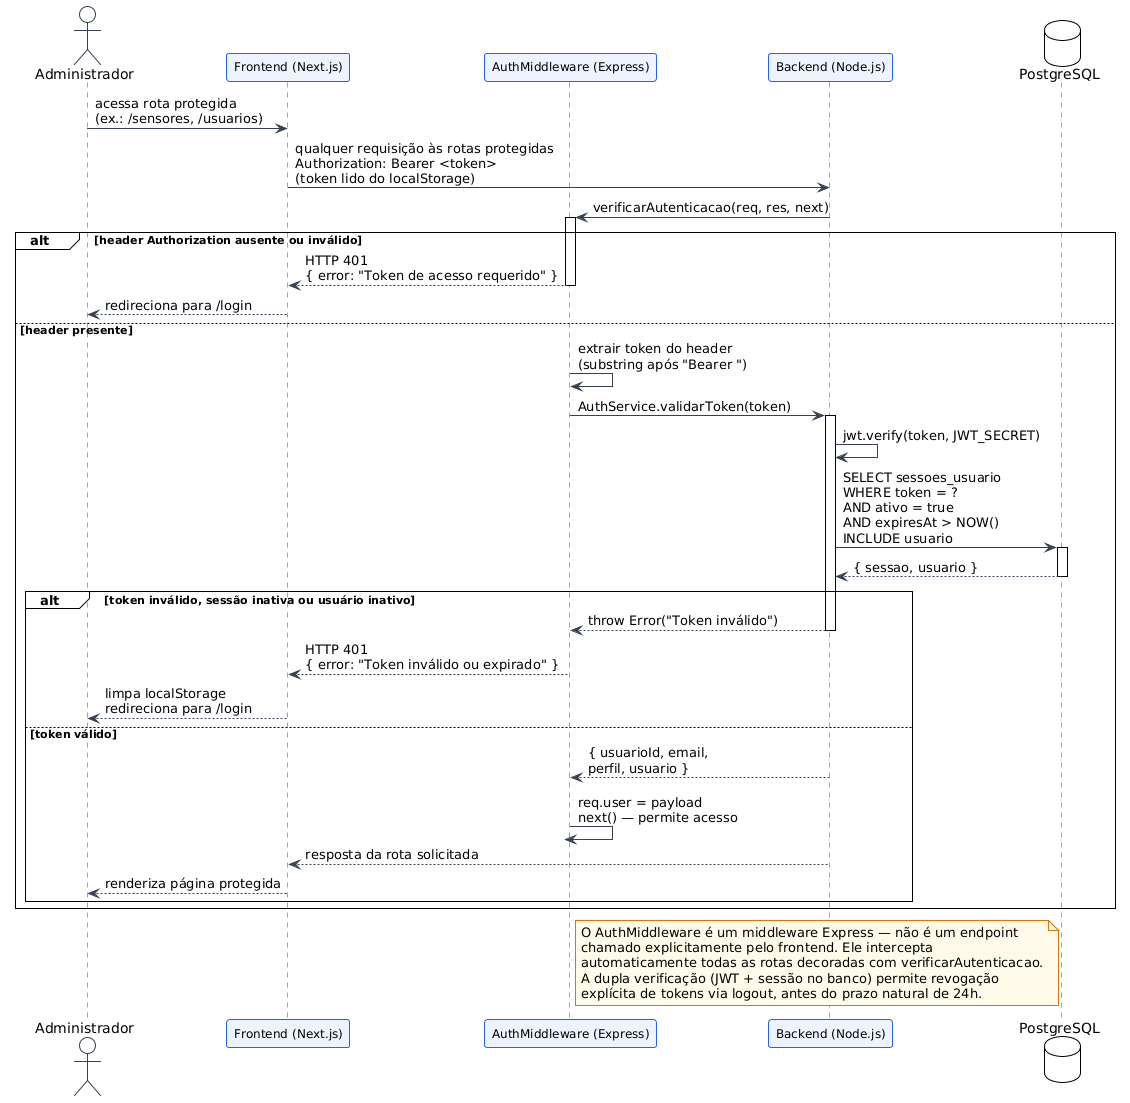
\includegraphics[width=0.85\textwidth]{figures/image55_seq_3b.png}
  \caption{Seq. 3b — Verificação de Rota Protegida}
  \label{fig:seq_3b}
  \fonte{Autora, 2025.}
\end{figure}

A Figura~\ref{fig:seq_3c} apresenta o fluxo de \textit{logout}. O
\texttt{AuthContext} invoca \texttt{authService.logout()}, que envia
\texttt{POST /auth/logout} ao \textit{backend} para marcar a sessão como inativa
no banco de dados. Independentemente do resultado dessa requisição, o bloco
\texttt{finally} do \texttt{AuthContext} garante a limpeza completa do estado
local: são removidas as entradas \texttt{'token'} e \texttt{'user'} do
\texttt{localStorage}, e os estados \texttt{user} e \texttt{isAuthenticated}
são zerados, assegurando que uma falha de rede não deixe dados de autenticação
residuais no navegador.

\begin{figure}[H]
  \centering
  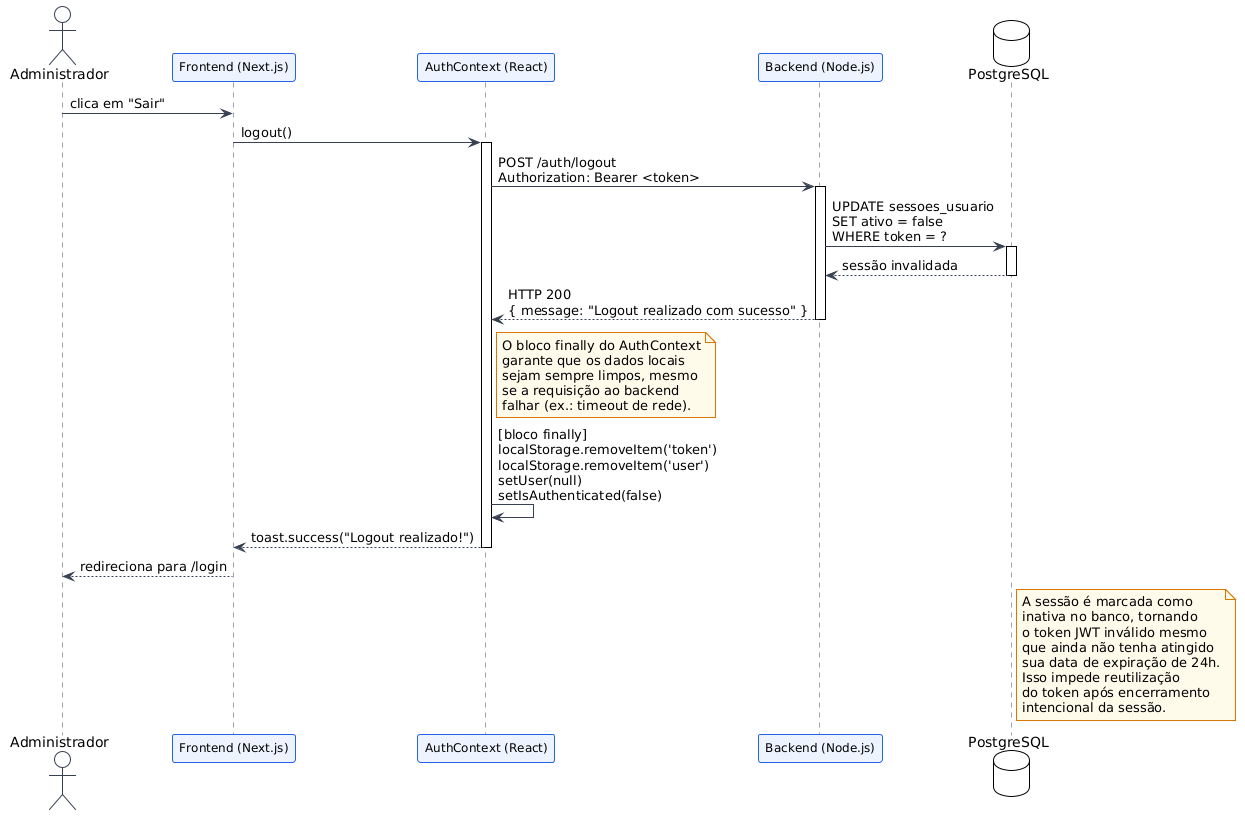
\includegraphics[width=0.85\textwidth]{figures/image55_seq_3c.png}
  \caption{Seq. 3c — Logout}
  \label{fig:seq_3c}
  \fonte{Autora, 2025.}
\end{figure}

% ─────────────────────────────────────────────────────────────
\subsubsubsection{Parte 4 — Recuperação de Senha}
% ─────────────────────────────────────────────────────────────

O fluxo de recuperação de senha é composto por três etapas sequenciais que garantem
a identidade do solicitante antes de permitir a alteração da credencial.

A Figura~\ref{fig:seq_4a} mostra a solicitação do token de \textit{reset}. O
\textit{backend} busca o usuário pelo e-mail informado e, independentemente de o
e-mail existir ou não no banco, retorna sempre HTTP 200 com a mensagem genérica
\textit{"Se o email existir, você receberá instruções para reset"} — medida que
impede que um atacante descubra quais endereços de e-mail estão cadastrados no
sistema. Quando o e-mail pertence a um usuário ativo, o \textit{backend} gera um
token de 64 caracteres hexadecimais via \texttt{crypto.randomBytes(32)}, persiste-o
no banco com validade de \textbf{duas horas} e aciona o \texttt{EmailService} para
envio do e-mail de recuperação. Quando o servidor SMTP não está configurado — cenário
típico em ambiente de desenvolvimento —, o \texttt{EmailService} opera em modo
simulação, registrando o token no console sem envio real, e o token é também
retornado na resposta da API para facilitar os testes. A validade de duas horas
é explicitamente exibida no \textit{template} HTML do e-mail enviado ao usuário.

\begin{figure}[H]
  \centering
  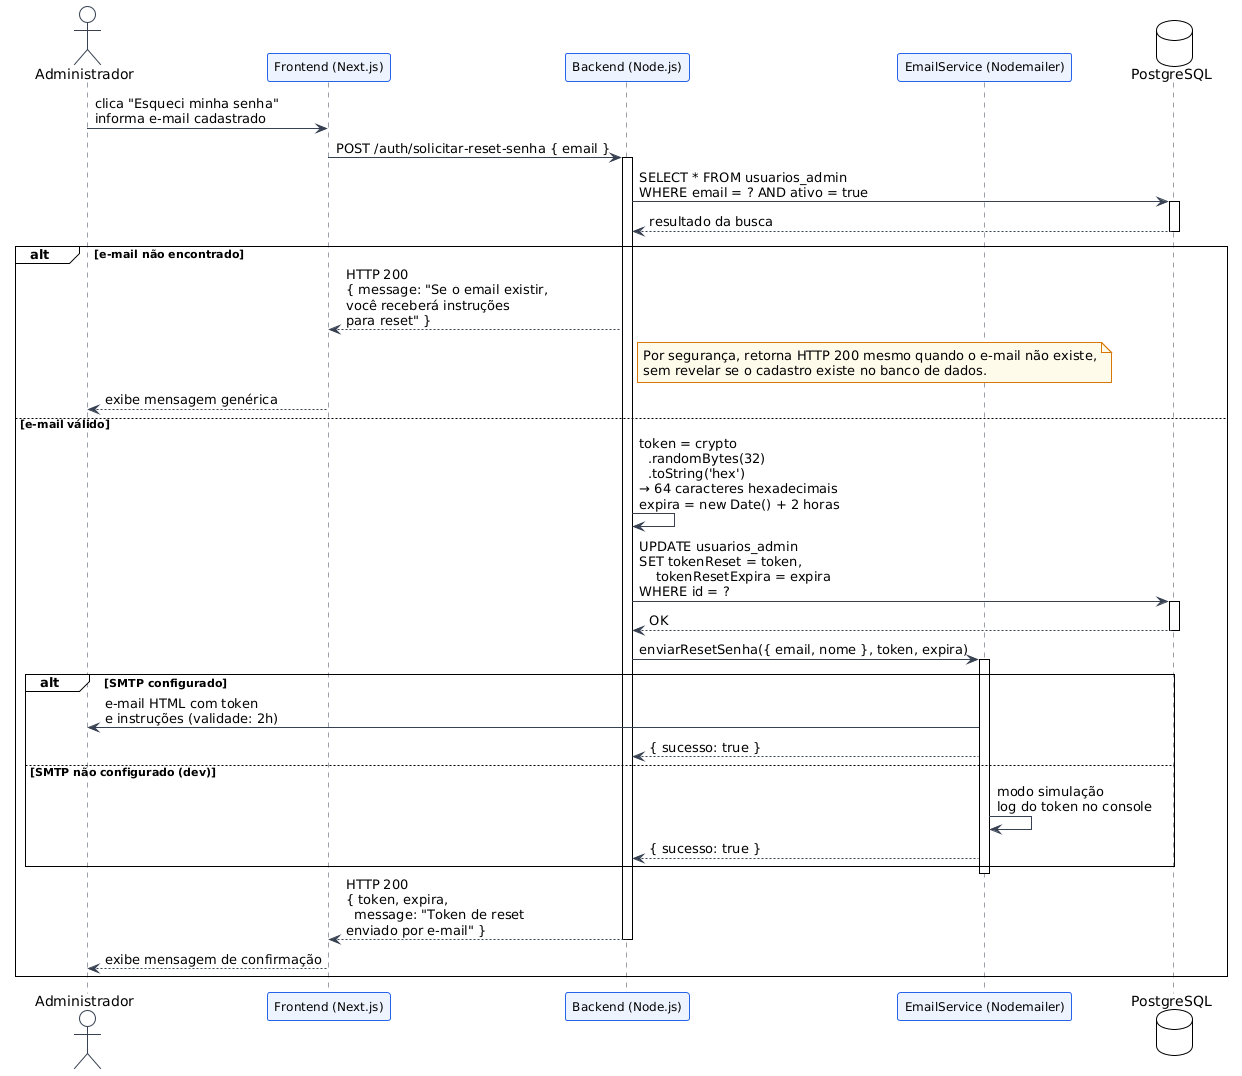
\includegraphics[width=0.85\textwidth]{figures/image55_seq_4a.png}
  \caption{Seq. 4a — Solicitação do Token de Reset}
  \label{fig:seq_4a}
  \fonte{Autora, 2025.}
\end{figure}

A Figura~\ref{fig:seq_4b} apresenta a validação do token. O frontend chama
\texttt{GET /auth/validar-token-reset/:token}, passando o token como parâmetro de
rota. O \textit{backend} verifica simultaneamente a existência do token no banco e
se o prazo de validade não foi ultrapassado, em uma única consulta que rejeita tokens
expirados mesmo que ainda existam no registro. A resposta de sucesso retorna apenas
\texttt{\{ valido: true, usuarioId \}}, sem expor nome ou e-mail do usuário.

\begin{figure}[H]
  \centering
  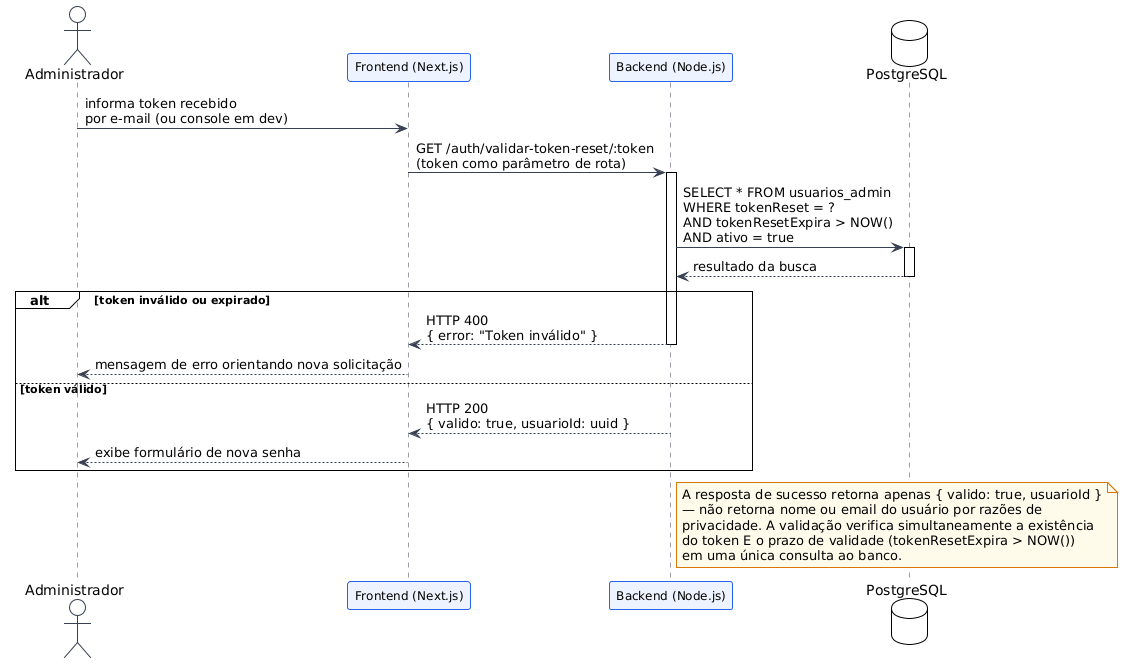
\includegraphics[width=0.85\textwidth]{figures/image55_seq_4b.png}
  \caption{Seq. 4b — Validação do Token de Reset}
  \label{fig:seq_4b}
  \fonte{Autora, 2025.}
\end{figure}

A Figura~\ref{fig:seq_4c} detalha a redefinição da senha. O \textit{payload}
enviado inclui \texttt{token}, \texttt{novaSenha} e \texttt{confirmarSenha}. Após
revalidação do token no banco, a nova senha é processada com
\texttt{bcrypt.hash(novaSenha, 10)} — os mesmos \textit{salt rounds} utilizados no
cadastro de usuários — e os campos \texttt{tokenReset} e \texttt{tokenResetExpira}
são zerados (\texttt{NULL}), tornando o token de uso único. Como medida de segurança
adicional, todas as sessões ativas do usuário são invalidadas no banco, exigindo novo
\textit{login} com a senha atualizada.

\begin{figure}[H]
  \centering
  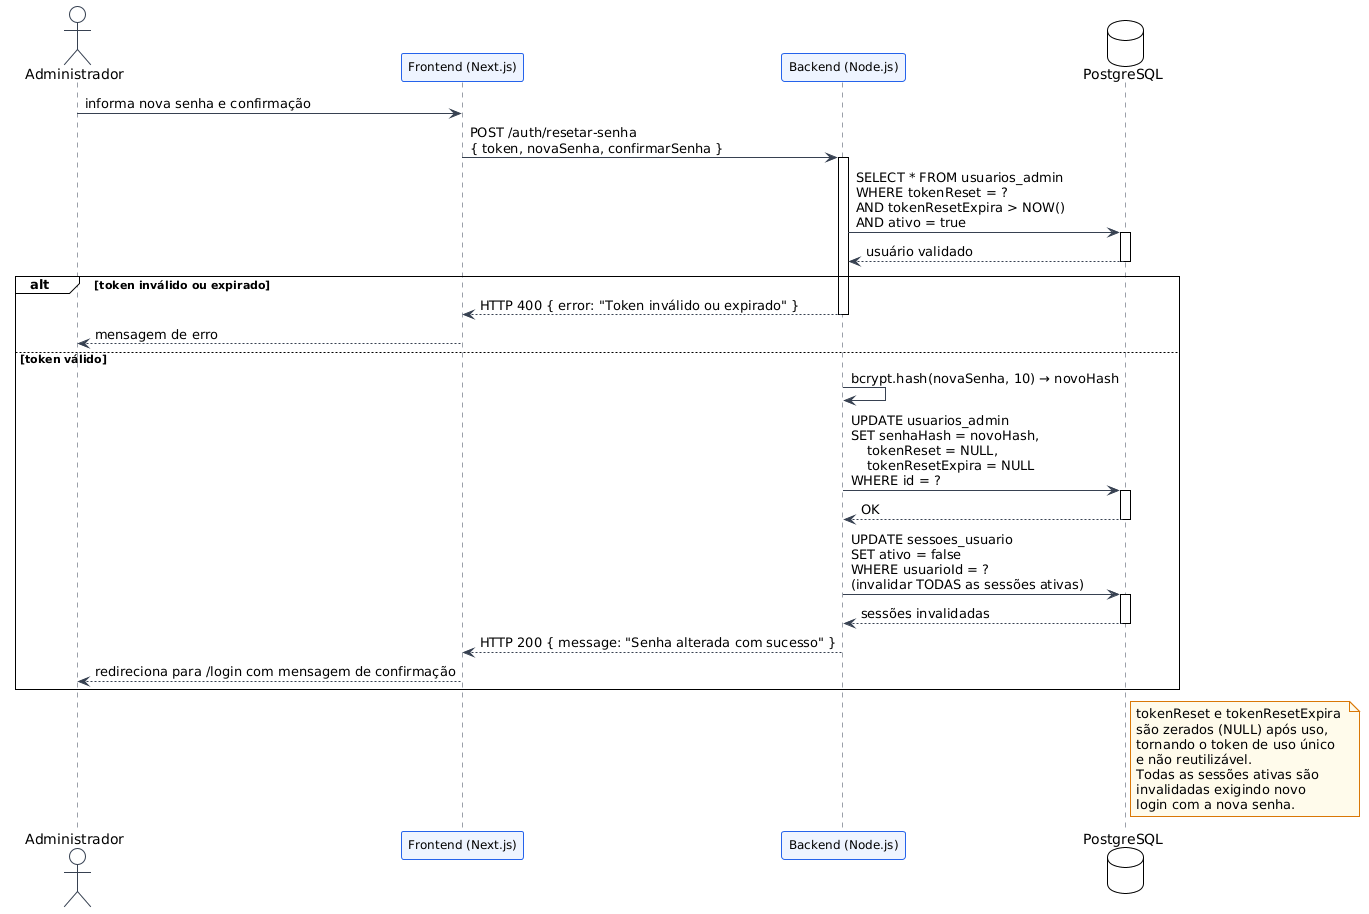
\includegraphics[width=0.85\textwidth]{figures/image55_seq_4c.png}
  \caption{Seq. 4c — Redefinição da Senha}
  \label{fig:seq_4c}
  \fonte{Autora, 2025.}
\end{figure}

% ─────────────────────────────────────────────────────────────
\subsubsubsection{Parte 5 — Dashboard e Monitoramento em Tempo Real}
% ─────────────────────────────────────────────────────────────

O painel de monitoramento é a tela principal da interface \textit{web} e combina
carregamento inicial em paralelo com mecanismos de atualização contínua.

A Figura~\ref{fig:seq_5a} apresenta o carregamento inicial do \textit{dashboard}.
O componente \texttt{DashboardContent} dispara quatro requisições simultâneas via
\texttt{Promise.all()} — estatísticas do sensor via \texttt{GET /sensor/estatisticas}
(sem parâmetro de período, retornando dados agregados padrão do serviço), estatísticas
de usuários, últimas 50 leituras para o gráfico temporal e os 10 alertas mais recentes.
Com os dados recebidos, são renderizados o card de situação atual com nível de alerta
e fator de risco percentual, cinco KPIs, o gráfico temporal interativo construído
com a biblioteca Recharts, o painel de alertas recentes, o card meteorológico e a
seção de atividade recente.

\begin{figure}[H]
  \centering
  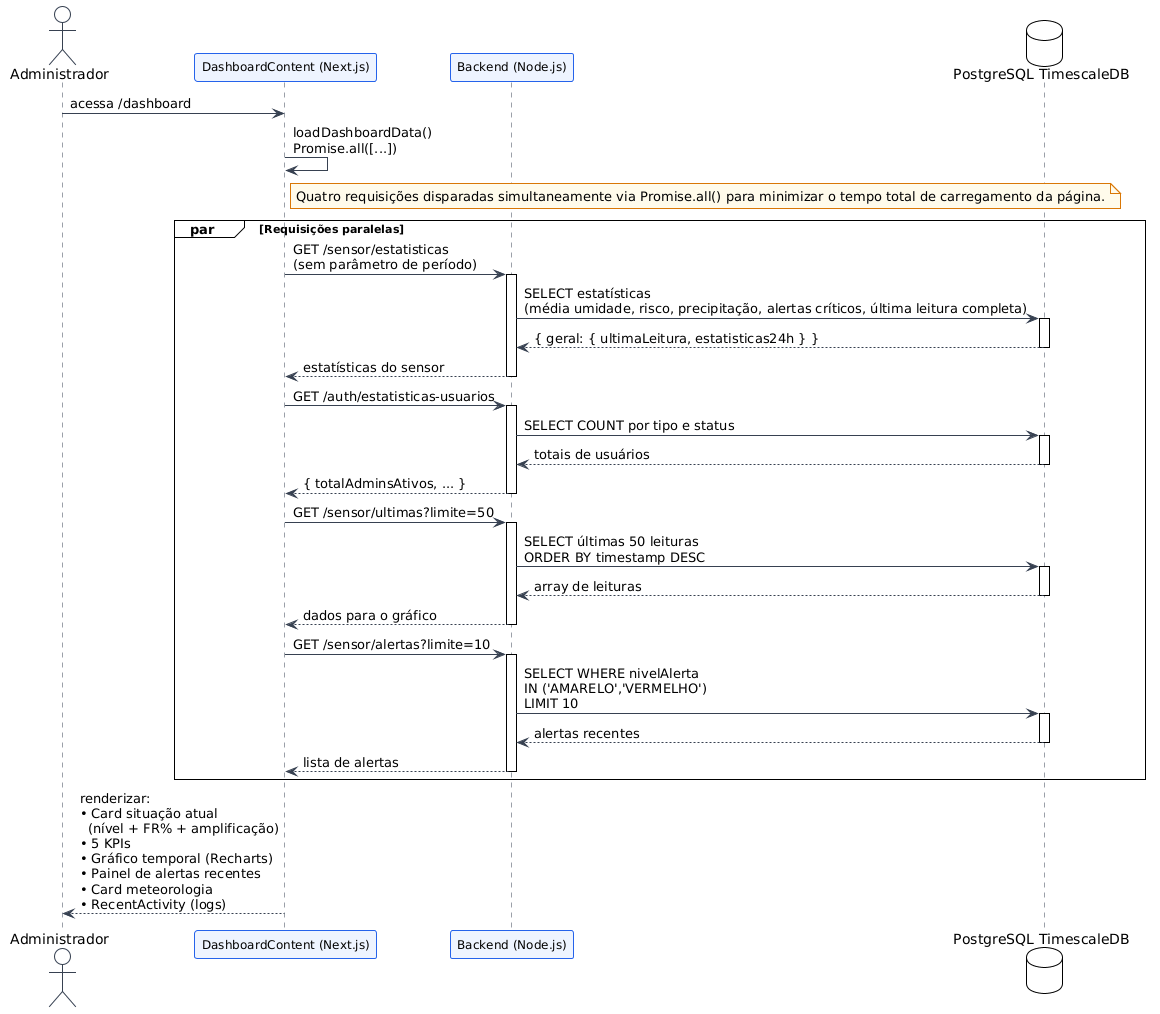
\includegraphics[width=0.85\textwidth]{figures/image55_seq_5a.png}
  \caption{Seq. 5a — Carregamento Inicial do Dashboard}
  \label{fig:seq_5a}
  \fonte{Autora, 2025.}
\end{figure}

A Figura~\ref{fig:seq_5b} ilustra os dois ciclos de \textit{polling} mantidos pelo
componente \texttt{Header}, ativos em todas as páginas da aplicação. O primeiro
consulta \texttt{GET /health} a cada 30 segundos para verificar a disponibilidade do
\textit{backend} e do banco de dados. O segundo consulta \texttt{GET /sensor/alertas}
a cada 60 segundos para atualizar o \textit{badge} do sino.

\begin{figure}[H]
  \centering
  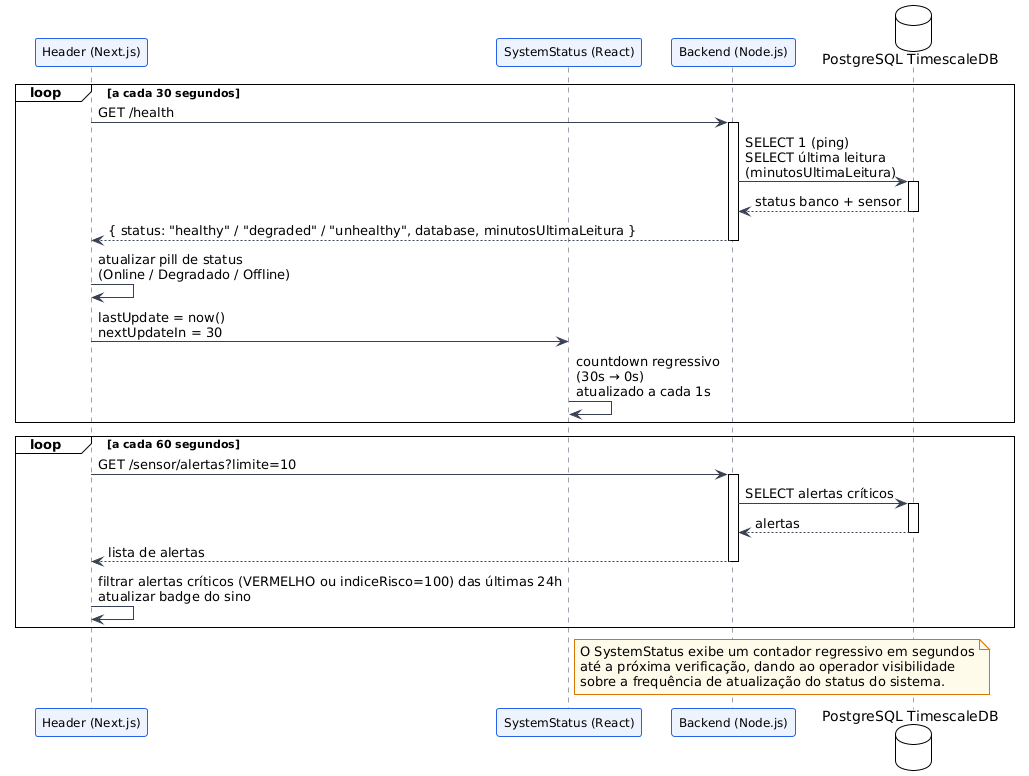
\includegraphics[width=0.85\textwidth]{figures/image55_seq_5b.png}
  \caption{Seq. 5b — Polling do Header (Health + Alertas)}
  \label{fig:seq_5b}
  \fonte{Autora, 2025.}
\end{figure}

A Figura~\ref{fig:seq_5c} mostra a interação com o sino de notificações. Ao clicar
no ícone, um \textit{dropdown} exibe os alertas mais recentes com nível, umidade,
fator de risco, confiabilidade e \textit{timestamp}. O \textit{badge} numérico
contabiliza apenas alertas críticos (VERMELHO ou RUPTURA) das últimas 24 horas.

\begin{figure}[H]
  \centering
  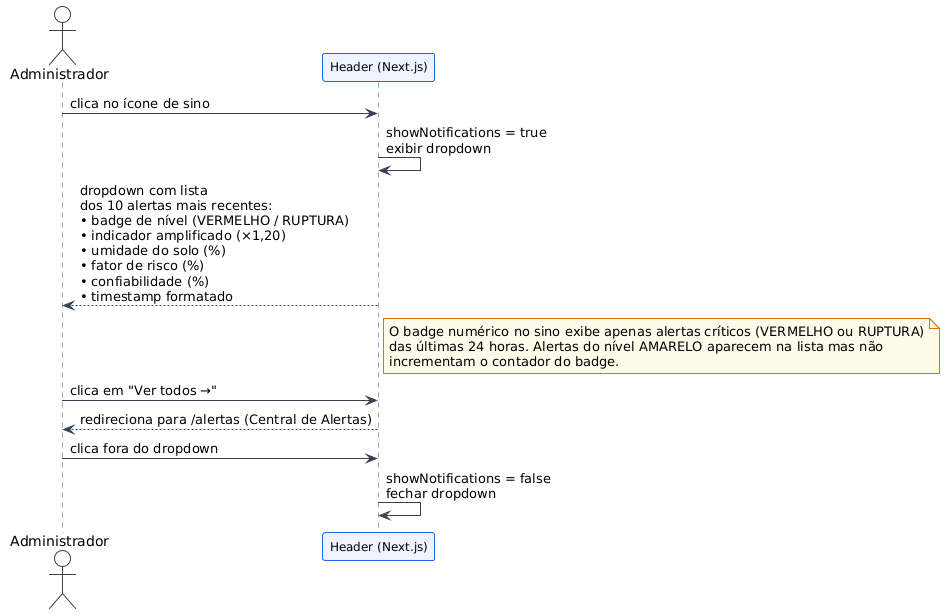
\includegraphics[width=0.85\textwidth]{figures/image55_seq_5c.png}
  \caption{Seq. 5c — Sino de Notificações}
  \label{fig:seq_5c}
  \fonte{Autora, 2025.}
\end{figure}

A Figura~\ref{fig:seq_5d} detalha o componente \texttt{RecentActivity}, que exibe
os dez registros mais recentes da tabela \texttt{logs\_sistema}, classificados por
componente de origem (SENSOR, BNDMET, OWM, CONECTIVIDADE) e nível de criticidade
(INFO, WARNING, ERROR, CRITICAL).

\begin{figure}[H]
  \centering
  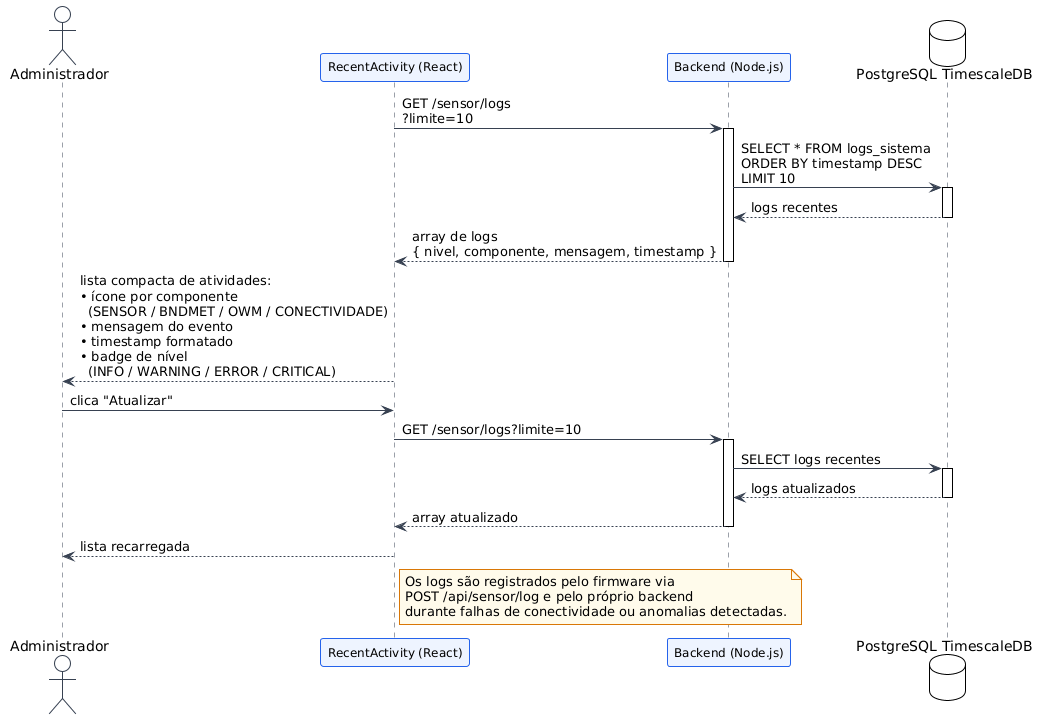
\includegraphics[width=0.85\textwidth]{figures/image55_seq_5d.png}
  \caption{Seq. 5d — RecentActivity (Logs do Sistema)}
  \label{fig:seq_5d}
  \fonte{Autora, 2025.}
\end{figure}

% ─────────────────────────────────────────────────────────────
\subsubsubsection{Parte 6 — Tela de Sensores, Filtros e Relatórios}
% ─────────────────────────────────────────────────────────────

A tela de sensores e o módulo de relatórios oferecem acesso ao histórico completo
de leituras com múltiplas formas de análise e exportação.

A Figura~\ref{fig:seq_6a} apresenta o carregamento da tela de sensores, que por
padrão exibe as leituras das últimas 24 horas via \texttt{GET /sensor/periodo}, com
até mil registros paginados a 15 por página na interface.

\begin{figure}[H]
  \centering
  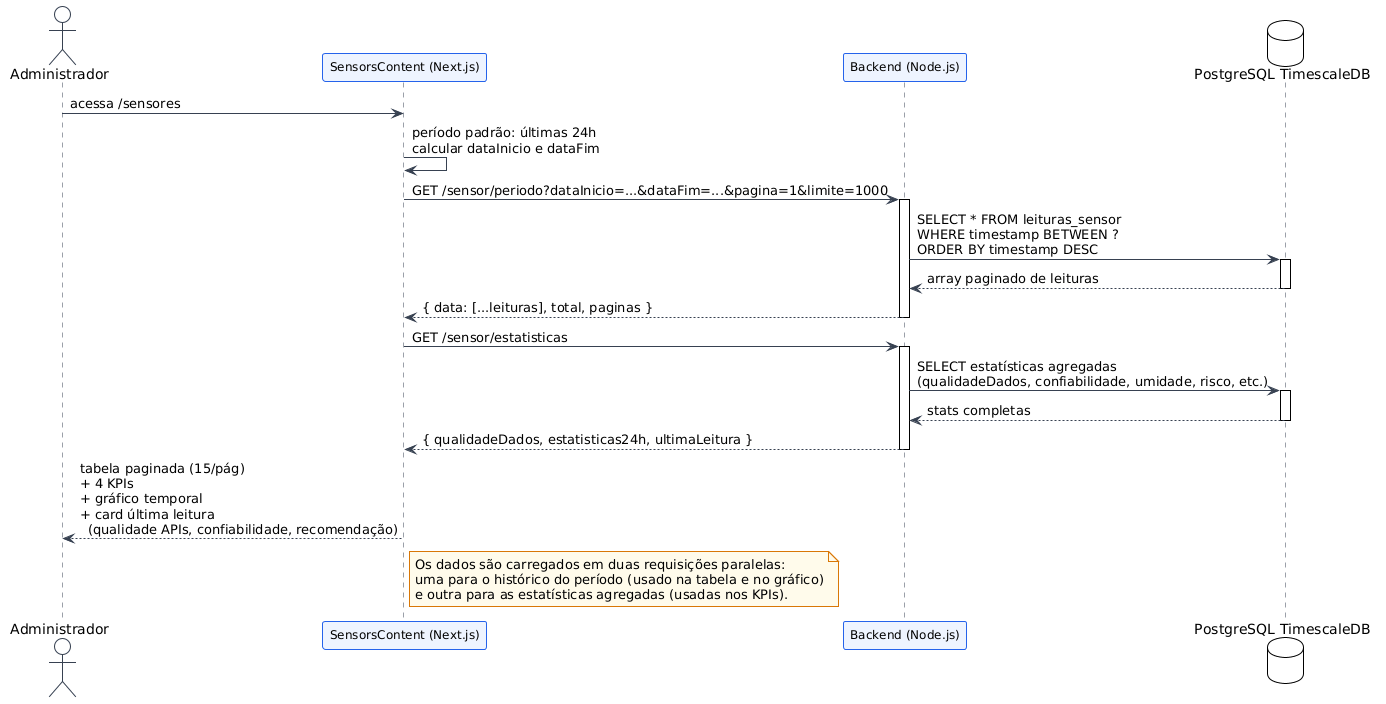
\includegraphics[width=0.85\textwidth]{figures/image55_seq_6a.png}
  \caption{Seq. 6a — Carregamento da Tela de Sensores}
  \label{fig:seq_6a}
  \fonte{Autora, 2025.}
\end{figure}

A Figura~\ref{fig:seq_6b} mostra os filtros de período e nível. A alteração de
período dispara uma nova requisição ao \textit{backend}, enquanto o filtro por nível
de alerta (TODOS, AMARELO, VERMELHO) é aplicado localmente sobre os dados em memória,
sem nova requisição. Os KPIs são recalculados sobre o subconjunto filtrado, não sobre
o total geral.

\begin{figure}[H]
  \centering
  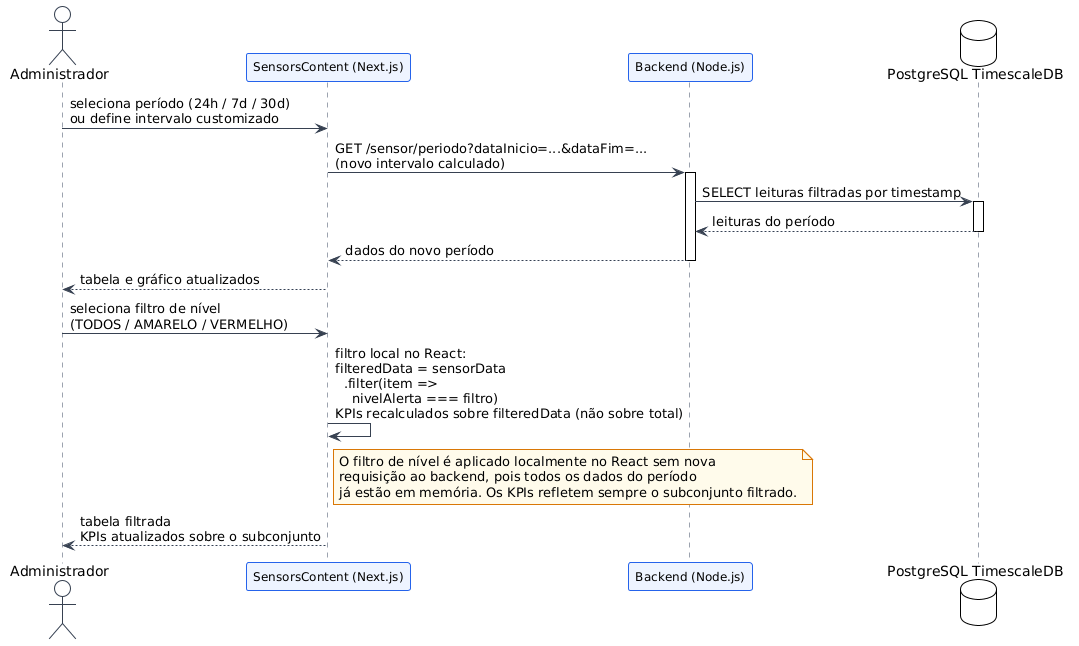
\includegraphics[width=0.85\textwidth]{figures/image55_seq_6b.png}
  \caption{Seq. 6b — Filtros de Período e Nível}
  \label{fig:seq_6b}
  \fonte{Autora, 2025.}
\end{figure}

A Figura~\ref{fig:seq_6c} detalha a linha expandida, exibida ao clicar em qualquer
registro da tabela. São apresentados quatro blocos: componentes individuais da
Equação~5 com a soma do fator de risco; contexto meteorológico completo da leitura;
dados de diagnóstico do firmware extraídos do campo \texttt{dadosBrutos}; e a
recomendação operacional gerada pelo firmware.

\begin{figure}[H]
  \centering
  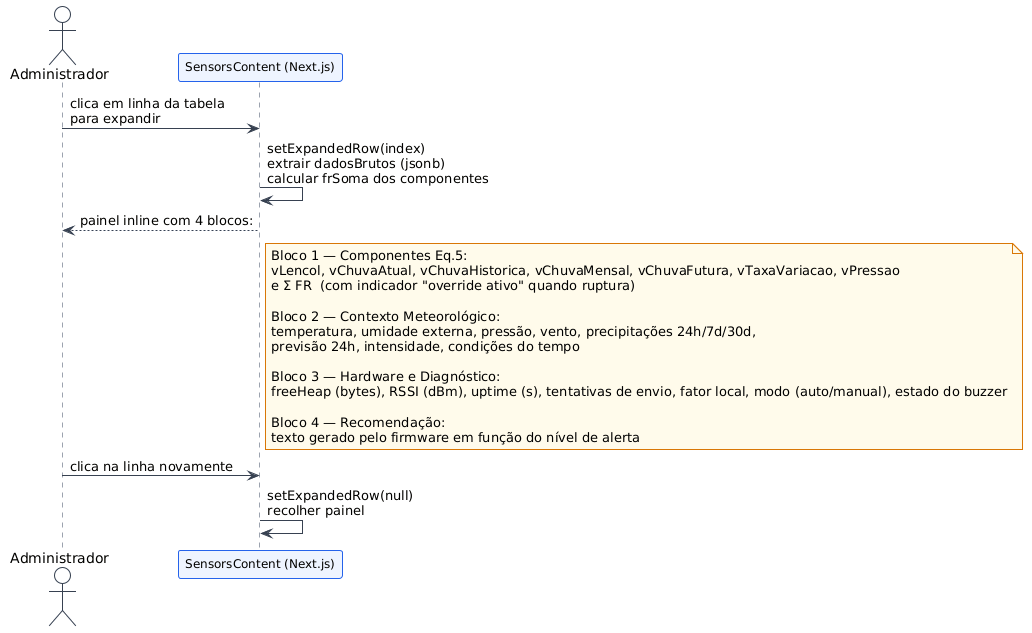
\includegraphics[width=0.85\textwidth]{figures/image55_seq_6c.png}
  \caption{Seq. 6c — Linha Expandida (Detalhamento da Leitura)}
  \label{fig:seq_6c}
  \fonte{Autora, 2025.}
\end{figure}

A Figura~\ref{fig:seq_6d} apresenta a exportação para CSV, que monta um arquivo com
mais de 40 colunas por linha cobrindo todos os campos da leitura e aciona o
\textit{download} automático no navegador, usando os dados já carregados em memória
sem nova requisição ao \textit{backend}.

\begin{figure}[H]
  \centering
  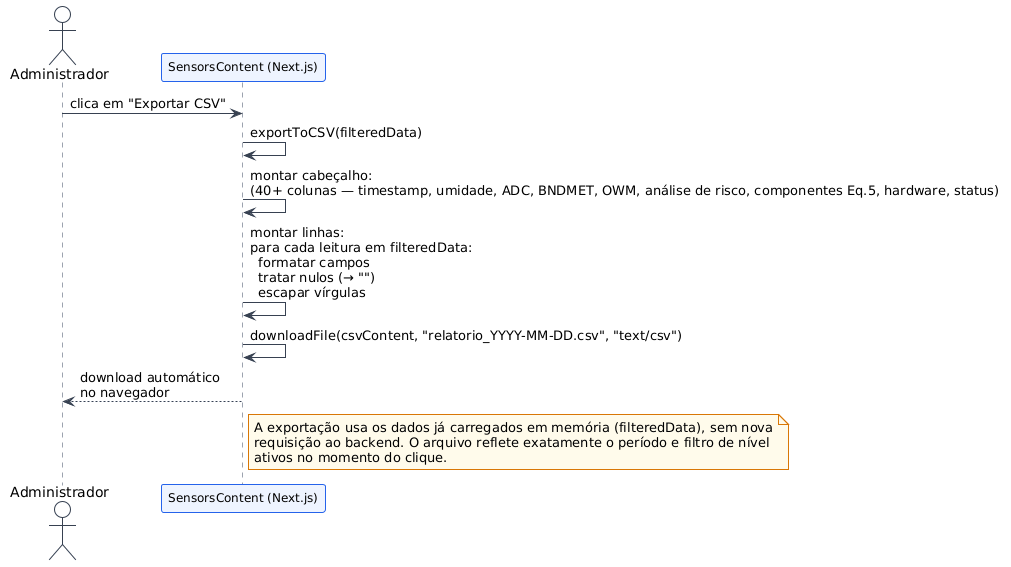
\includegraphics[width=0.85\textwidth]{figures/image55_seq_6d.png}
  \caption{Seq. 6d — Exportação CSV}
  \label{fig:seq_6d}
  \fonte{Autora, 2025.}
\end{figure}

A Figura~\ref{fig:seq_6e} ilustra a geração de relatório pelo módulo
\texttt{ReportsContent}. Os dados do período consultado são processados localmente
para calcular estatísticas descritivas de cada variável monitorada, organizadas em seis
seções. O relatório pode ser exportado em CSV ou em HTML autossuficiente com estilos
\textit{inline}, adequado para arquivamento e distribuição sem dependências externas.

\begin{figure}[H]
  \centering
  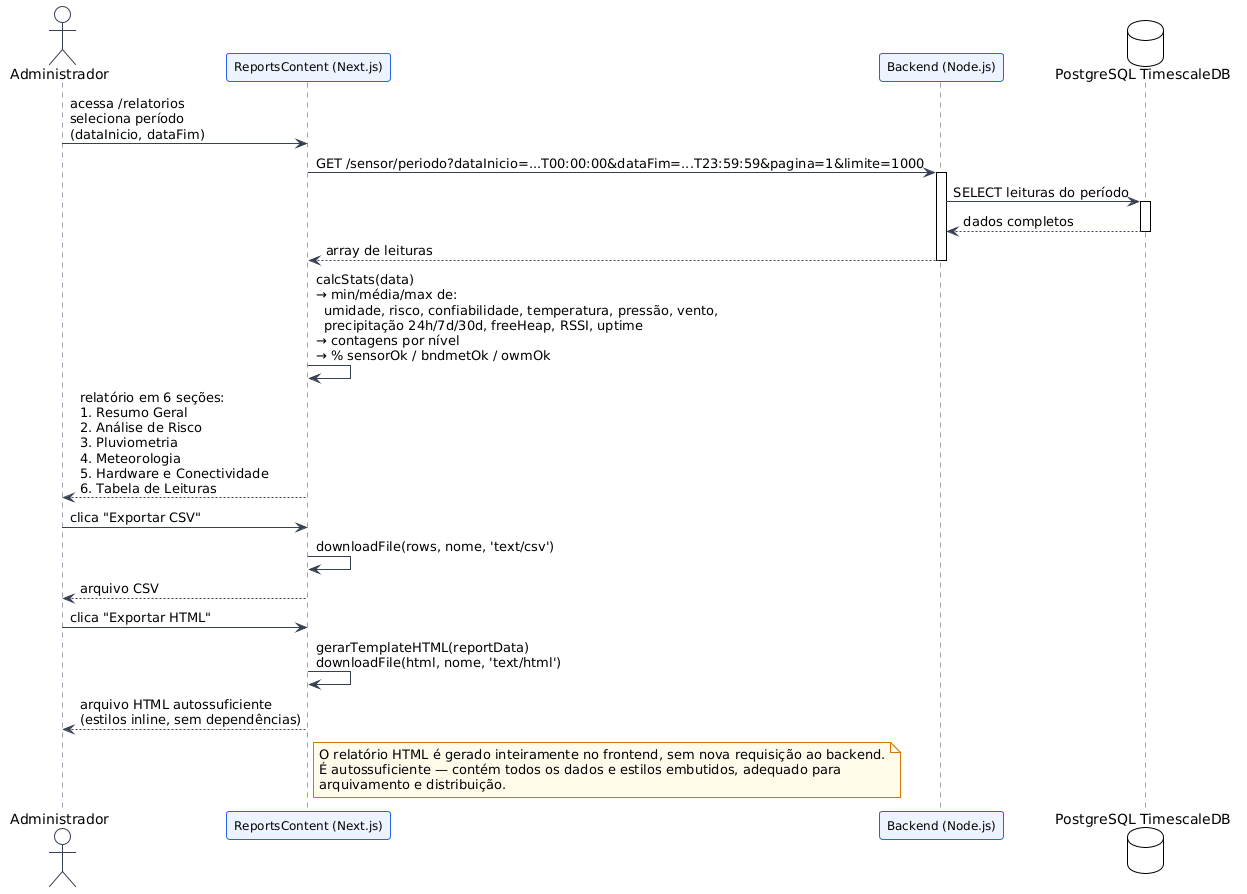
\includegraphics[width=0.85\textwidth]{figures/image55_seq_6e.png}
  \caption{Seq. 6e — Geração de Relatório}
  \label{fig:seq_6e}
  \fonte{Autora, 2025.}
\end{figure}

% ─────────────────────────────────────────────────────────────
\subsubsubsection{Parte 7 — Gestão de Usuários e Central de Alertas}
% ─────────────────────────────────────────────────────────────

O módulo de gestão de usuários e a central de alertas compõem o conjunto de
funcionalidades administrativas do sistema.

A Figura~\ref{fig:seq_7a} apresenta o carregamento da tela de usuários. A listagem
principal exibe apenas usuários com \texttt{ativo = true}, passado como parâmetro
\texttt{ativo: true} na requisição de listagem. A paginação padrão é de 10 registros
por página. A tela alterna entre as abas de usuários básicos e administradores,
disparando nova requisição ao trocar de aba. Usuários inativos são acessíveis
exclusivamente pelo modal específico de inativos, não pela tabela principal.

\begin{figure}[H]
  \centering
  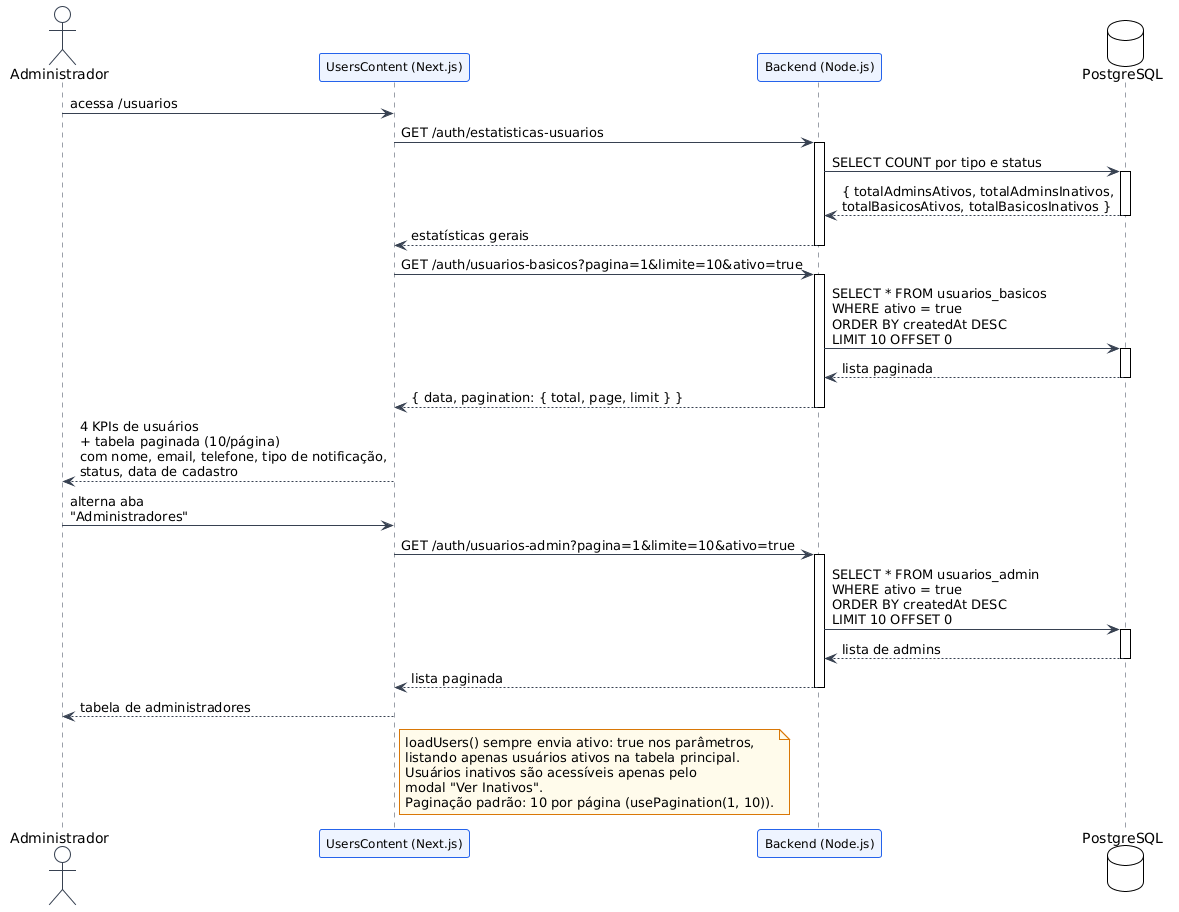
\includegraphics[width=0.85\textwidth]{figures/image55_seq_7a.png}
  \caption{Seq. 7a — Listagem e Estatísticas de Usuários}
  \label{fig:seq_7a}
  \fonte{Autora, 2025.}
\end{figure}

A Figura~\ref{fig:seq_7b} detalha os fluxos de criação e edição de usuário. A
criação de usuário básico utiliza o endpoint público \texttt{POST /auth/cadastro-basico},
que não requer autenticação, e inclui o campo \texttt{senha} no \textit{payload}
além dos dados de perfil. A criação de administrador utiliza
\texttt{POST /auth/cadastro-admin}, rota protegida pelo \textit{middleware}
\texttt{verificarSuperAdmin} — somente administradores com perfil
\texttt{super\_admin} podem criar novos administradores. Ambos os formulários
são gerenciados pelo componente \texttt{UserForm}, reutilizado tanto para criação
(modal vazio) quanto para edição (modal pré-preenchido).

\begin{figure}[H]
  \centering
  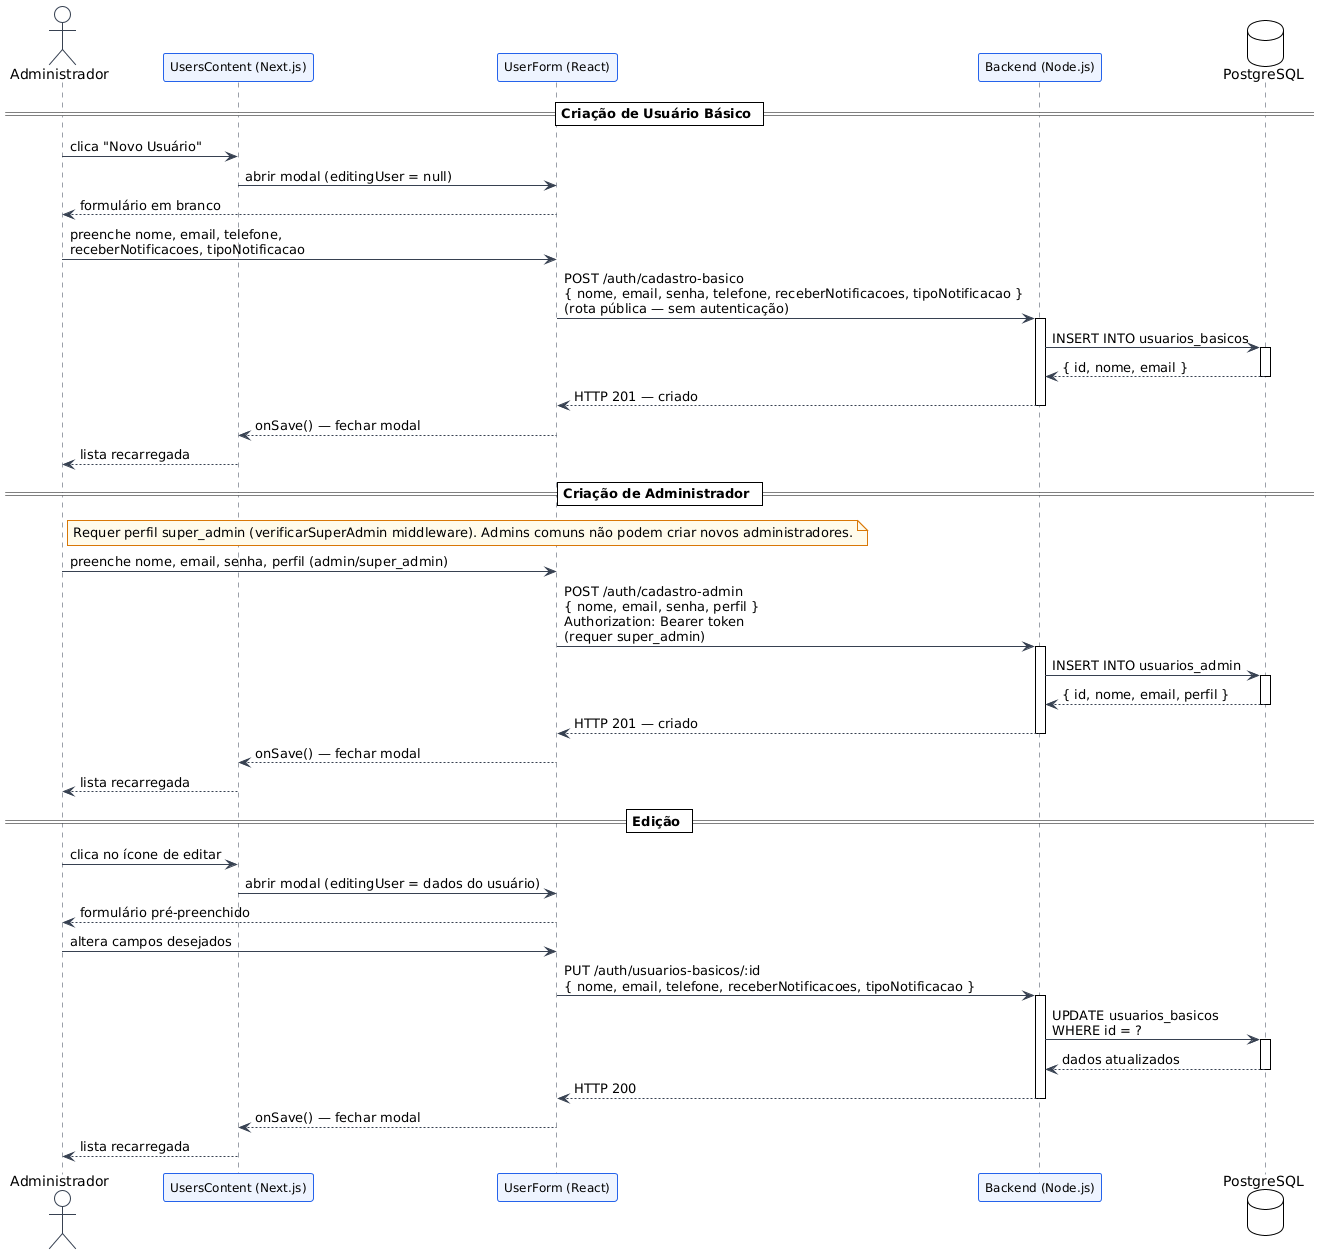
\includegraphics[width=0.85\textwidth]{figures/image55_seq_7b.png}
  \caption{Seq. 7b — Criação e Edição de Usuário}
  \label{fig:seq_7b}
  \fonte{Autora, 2025.}
\end{figure}

A Figura~\ref{fig:seq_7c} apresenta os fluxos de desativação e reativação de
usuários. A desativação utiliza o verbo HTTP \texttt{DELETE}, porém implementa
deleção lógica no banco de dados: o registro não é removido, apenas o campo
\texttt{ativo} é atualizado para \texttt{false}, preservando o histórico de alertas
recebidos pelo usuário. Para administradores, o serviço verifica se o alvo não é o
último \texttt{super\_admin} ativo do sistema antes de prosseguir com a desativação,
e impede que um administrador desative a própria conta. A reativação é feita pelo
modal de usuários inativos, que carrega via \texttt{GET /auth/usuarios-inativos}
o conjunto unificado de usuários básicos e administradores com \texttt{ativo = false}.
Após a reativação bem-sucedida, o usuário é removido da lista do modal localmente,
sem nova requisição, e o componente pai recarrega as estatísticas.

\begin{figure}[H]
  \centering
  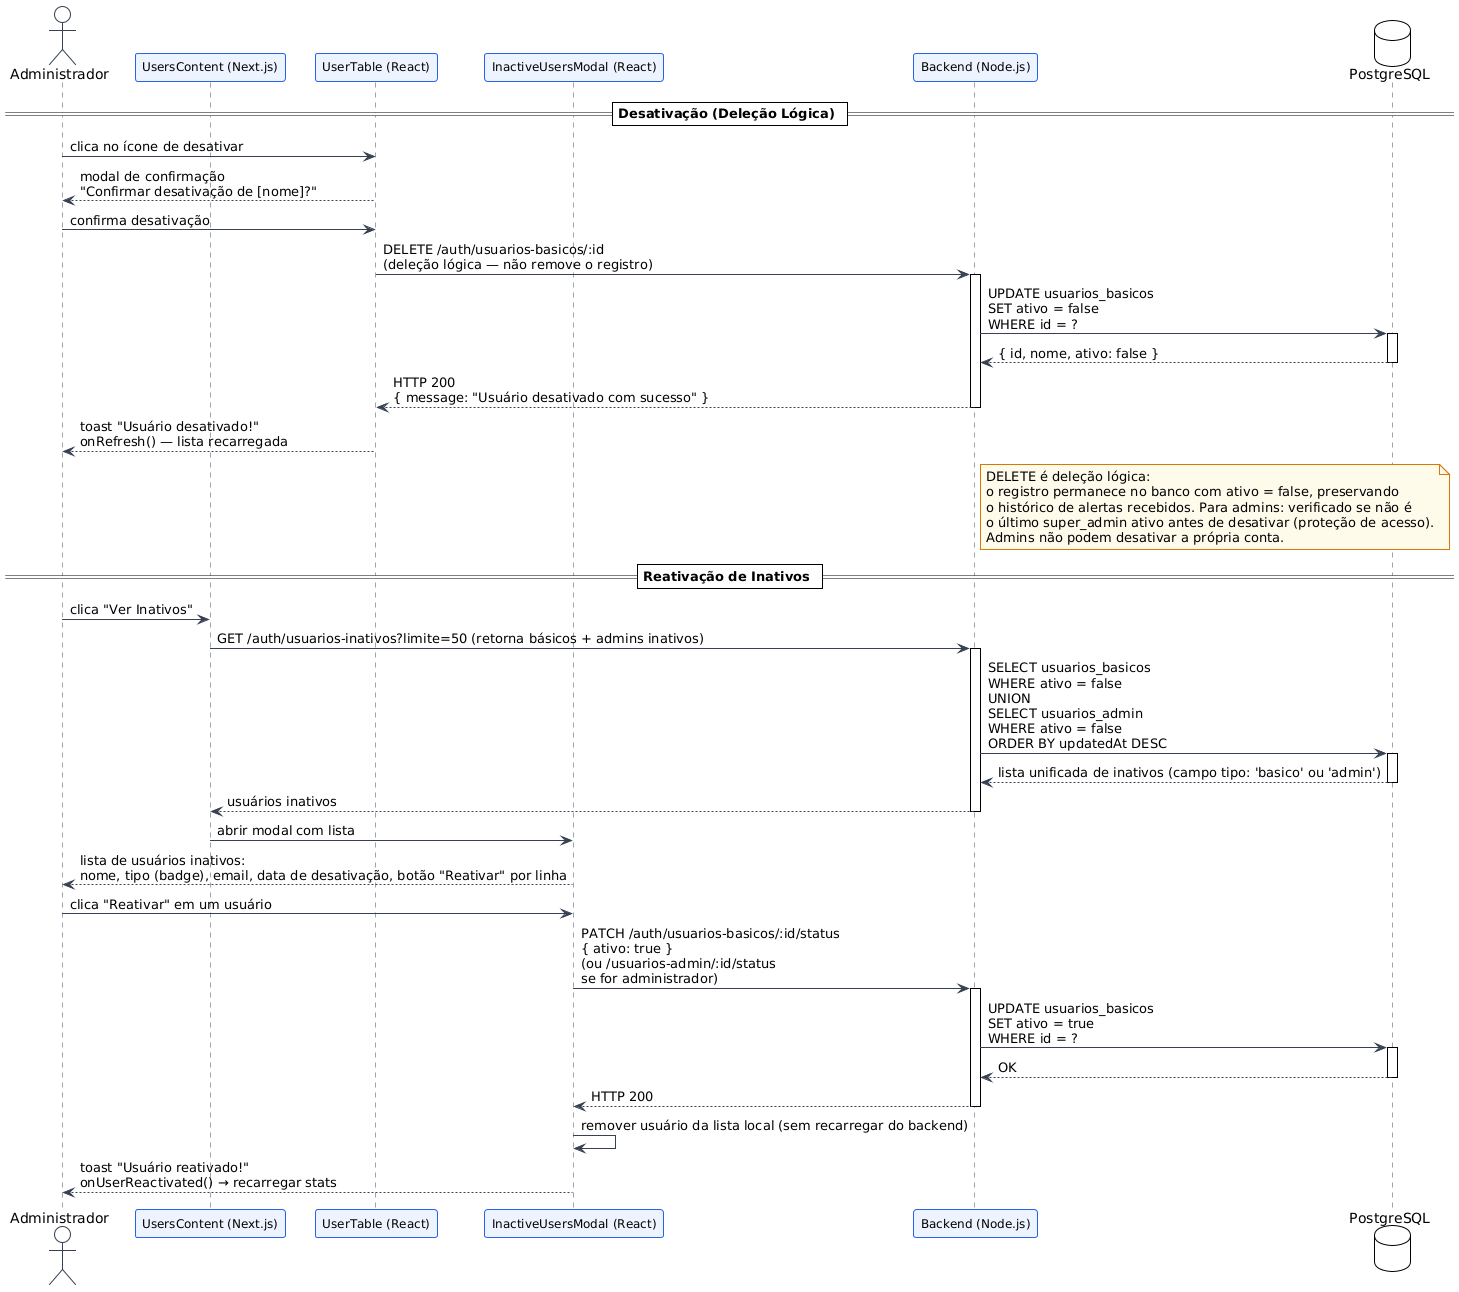
\includegraphics[width=0.85\textwidth]{figures/image55_seq_7c.png}
  \caption{Seq. 7c — Desativação e Reativação de Usuários Inativos}
  \label{fig:seq_7c}
  \fonte{Autora, 2025.}
\end{figure}

A Figura~\ref{fig:seq_7d} ilustra o carregamento da Central de Alertas e a expansão
de um alerta para visualização de detalhes. São carregados até 200 alertas ativos,
com KPIs de contagem por categoria e paginação a 10 por página. Ao expandir um
alerta, são exibidos os blocos de componentes da Equação~5, contexto meteorológico,
hardware e diagnóstico, e o cálculo detalhado de confiabilidade — com os descontos
individuais por fonte de dados indisponível, ou a indicação de estado especial de
RUPTURA quando a confiabilidade está fixada em 100\% por confirmação direta do
hardware.

\begin{figure}[H]
  \centering
  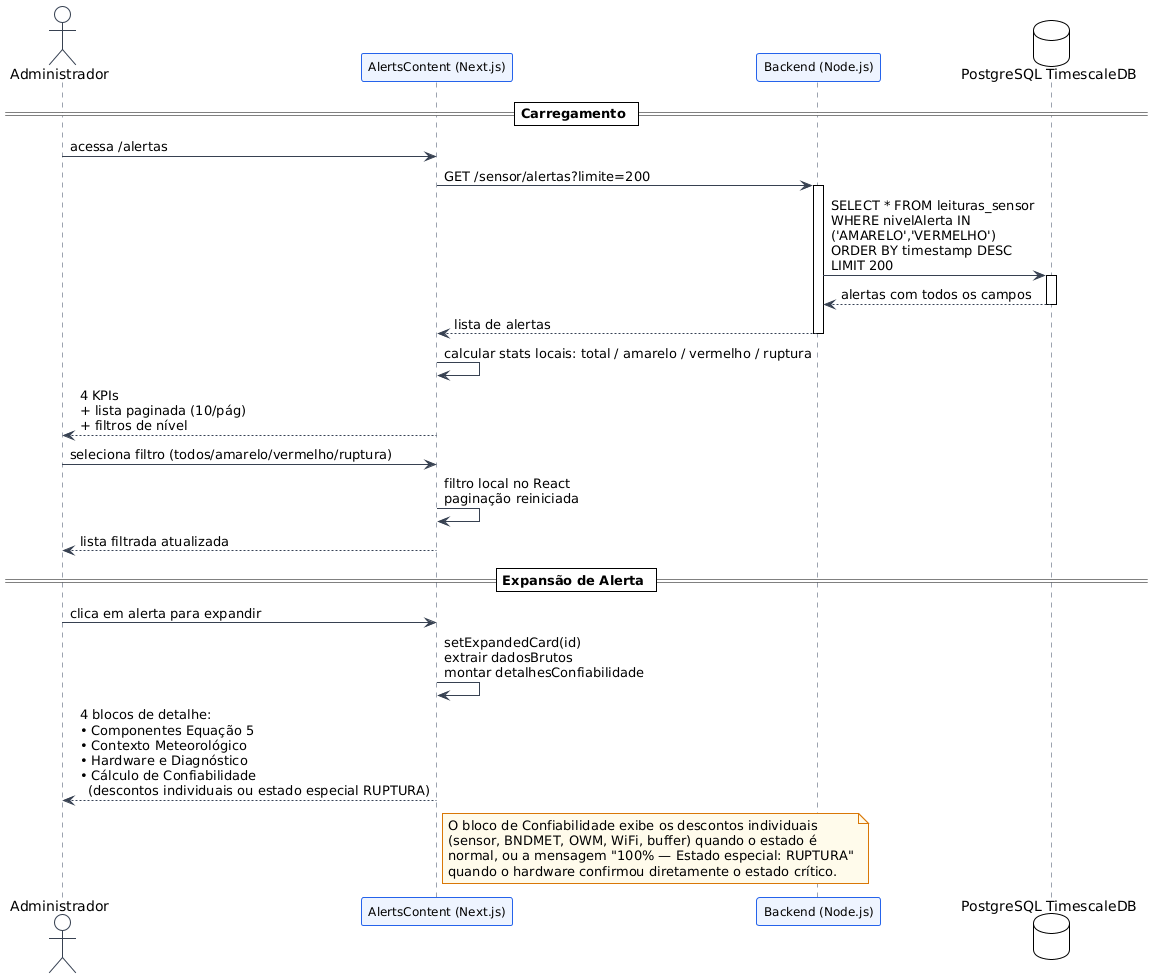
\includegraphics[width=0.85\textwidth]{figures/image55_seq_7d.png}
  \caption{Seq. 7d — Central de Alertas: Carregamento e Expansão}
  \label{fig:seq_7d}
  \fonte{Autora, 2025.}
\end{figure}

A Figura~\ref{fig:seq_7e} detalha o envio de alerta em massa. Após confirmação pelo
administrador, o \textit{backend} consulta todos os usuários básicos ativos com
notificações habilitadas e processa o envio via \texttt{EmailService.enviarLote()}.
Quando o servidor SMTP está configurado, os e-mails são enviados de forma real com
\textit{template} HTML colorizado conforme o nível de criticidade. Quando o SMTP não
está disponível — cenário de desenvolvimento —, o método privado
\texttt{simularEnvioAlertas()} registra o disparo no console e retorna sucesso
simulado para todos os destinatários, sem envio efetivo. Em ambos os cenários, o
resultado completo da operação é persistido na tabela \texttt{logs\_alertas} com os
totais de sucesso e falha e o campo \texttt{detalhesEnvio} (\textit{jsonb}) contendo
o resultado individual de cada destinatário, criando uma trilha de auditoria completa
de todas as notificações disparadas pelo sistema.

\begin{figure}[H]
  \centering
  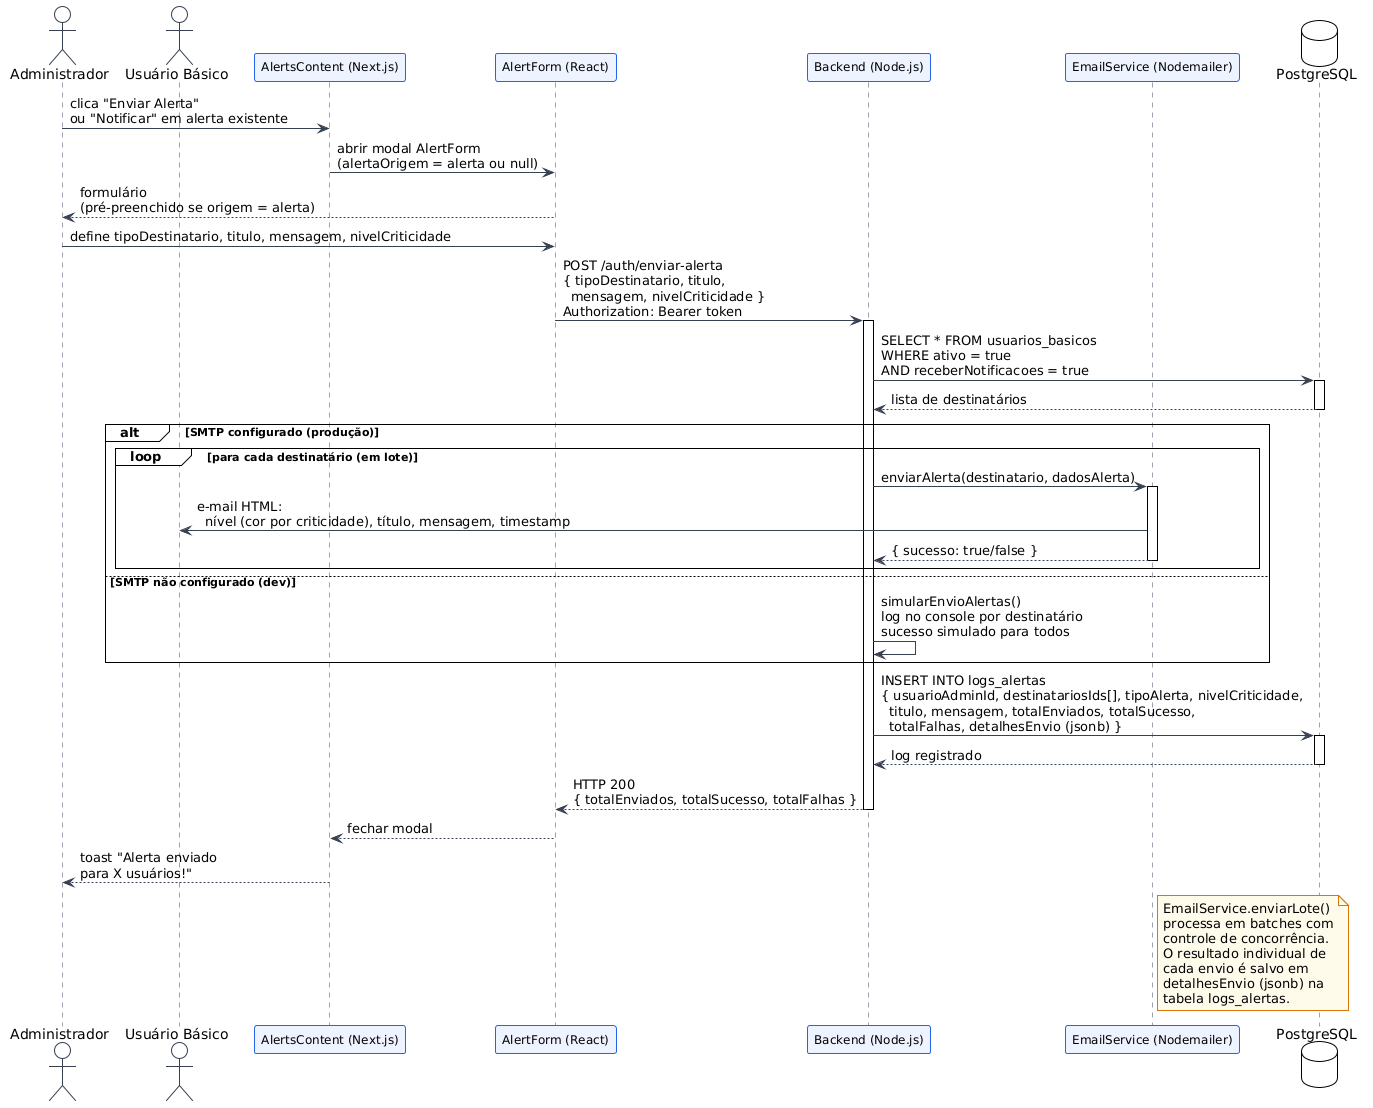
\includegraphics[width=0.85\textwidth]{figures/image55_seq_7e.png}
  \caption{Seq. 7e — Envio de Alerta em Massa}
  \label{fig:seq_7e}
  \fonte{Autora, 2025.}
\end{figure}

% -------------------------------------------------------------
\subsubsection{Diagramas de Lógica do Sistema}
\label{subsubsubsec:diagramas-logica}
% -------------------------------------------------------------

Os fluxogramas apresentados nesta seção representam processos do
sistema que envolvem decisões condicionais relevantes para a
compreensão do comportamento operacional. 

Foram elaborados nove fluxogramas, distribuídos entre
as três camadas da arquitetura. A Figura~\ref{fig:fluxograma_visao_geral}
apresenta o mapa geral com os identificadores e as relações entre
os diagramas.

\begin{figure}[htb]
\centering
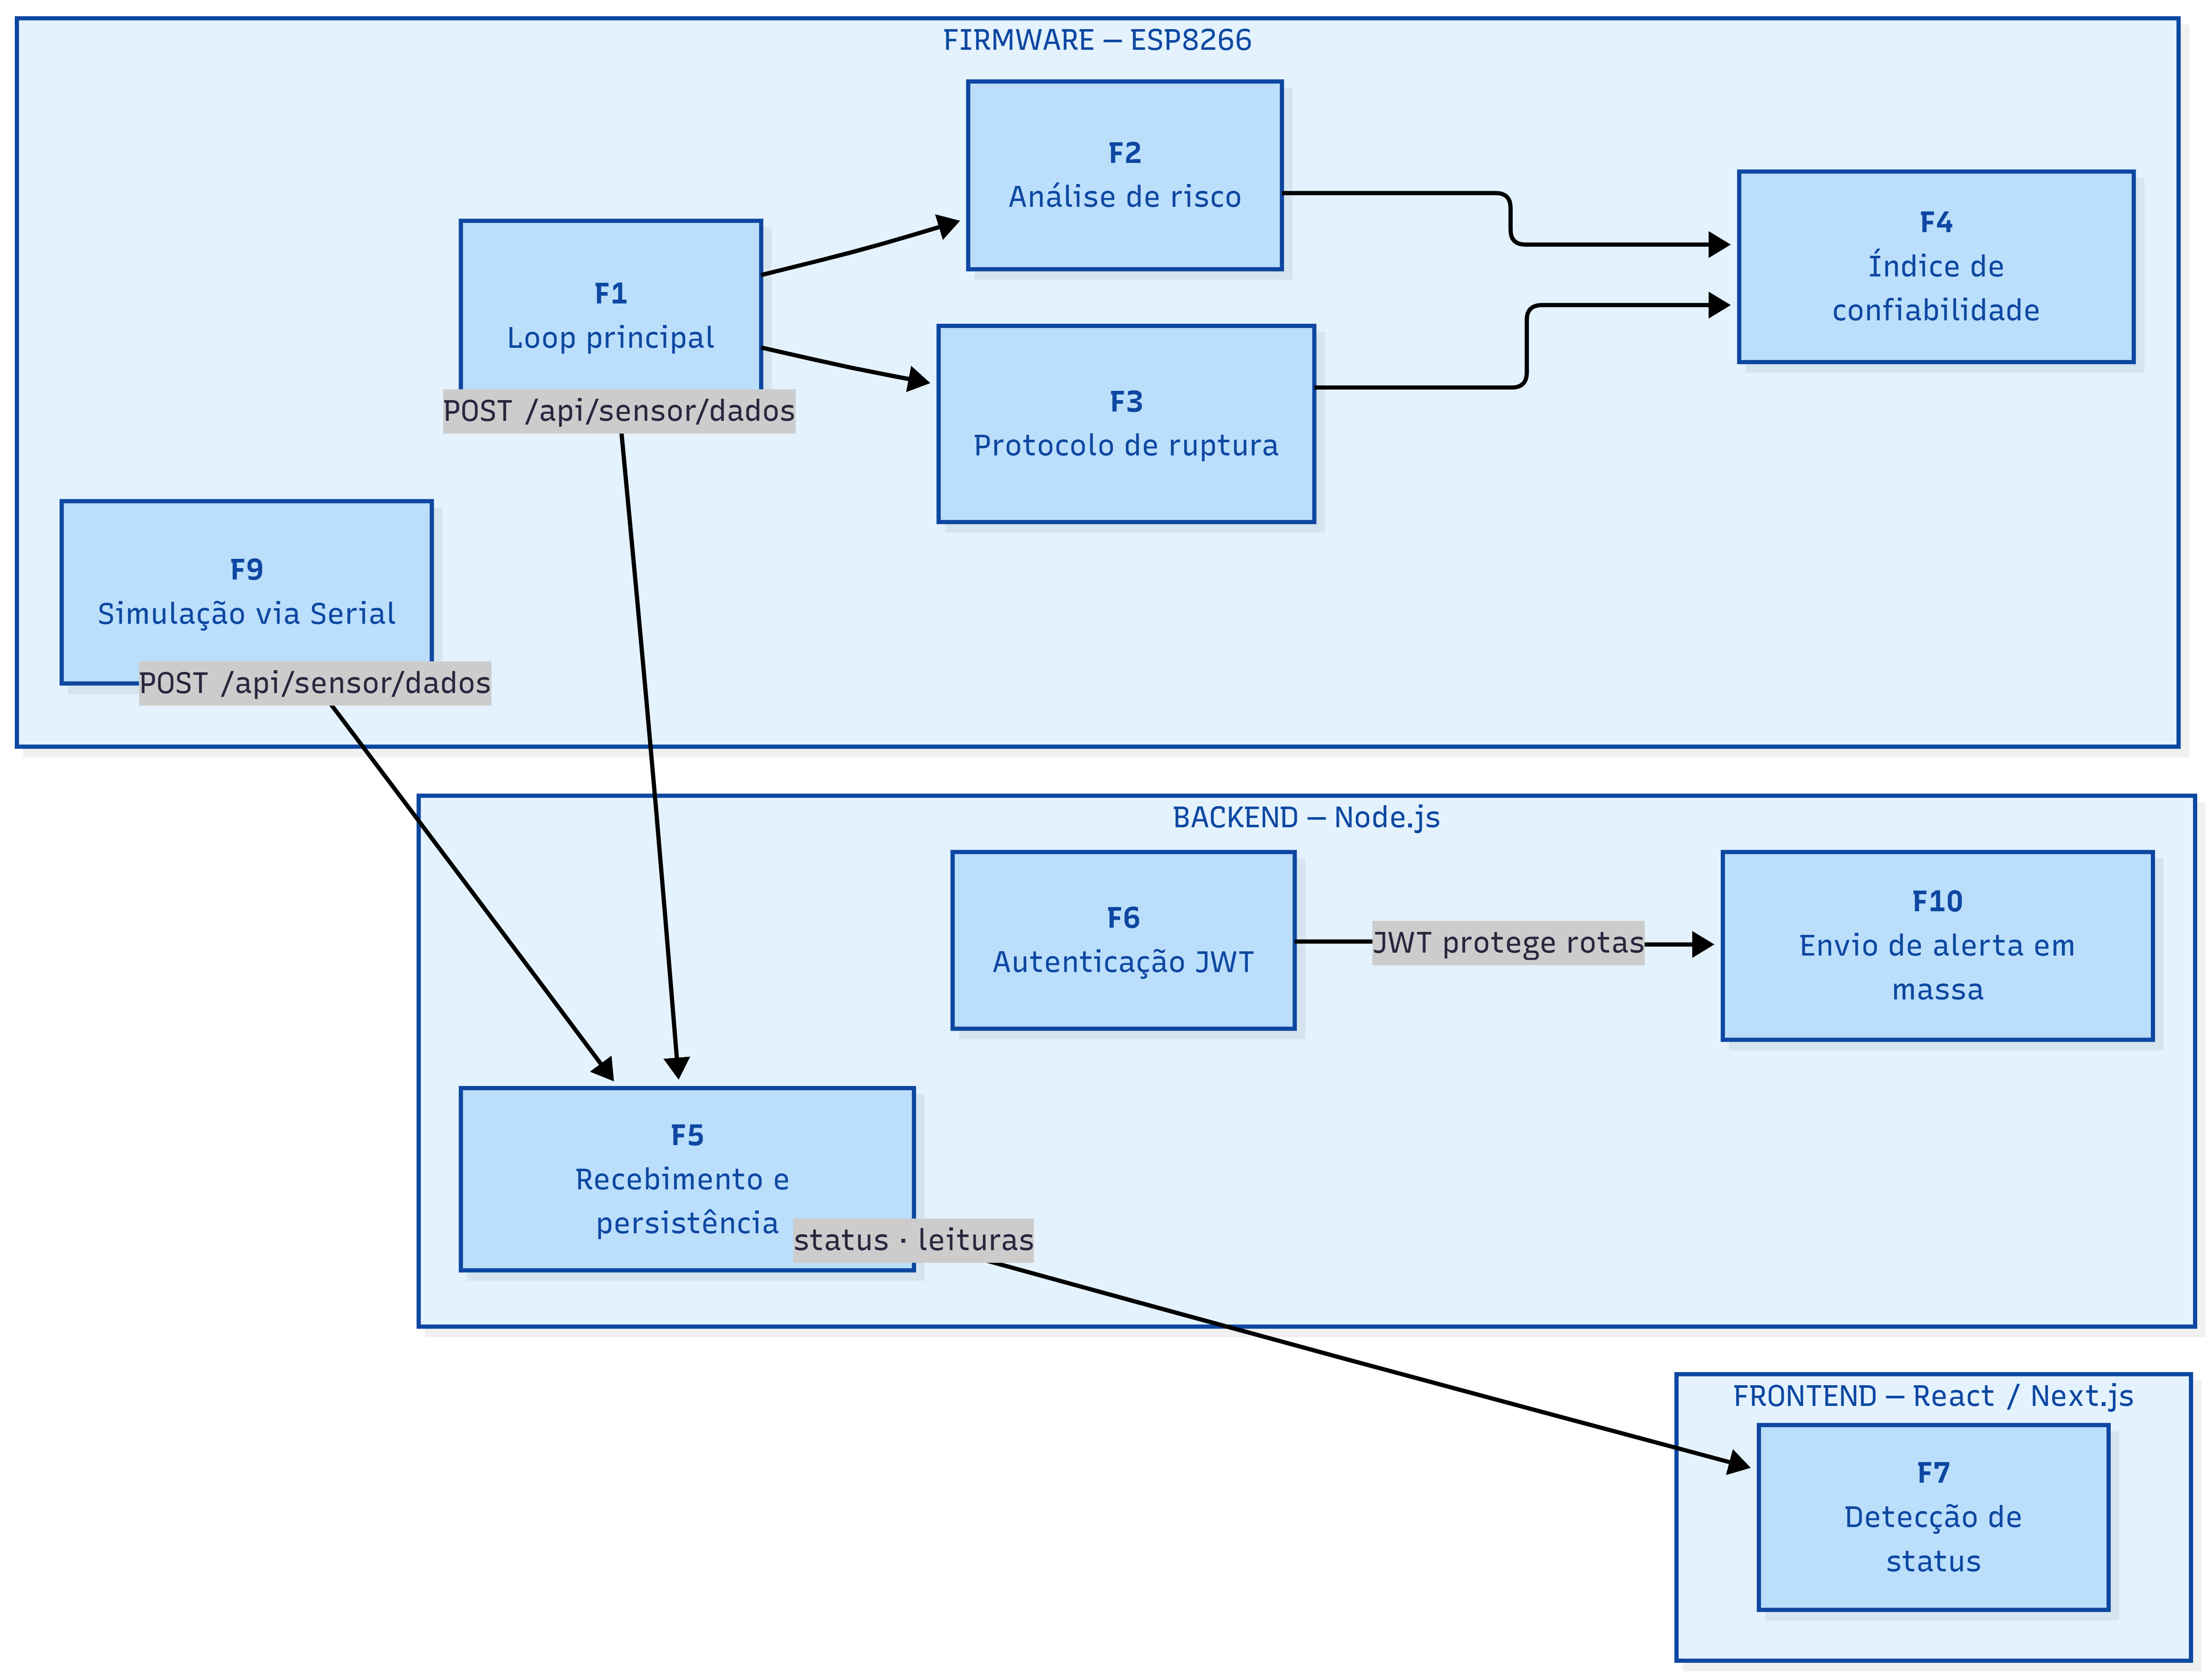
\includegraphics[width=\textwidth]
    {figures/cap4_fluxograma_f0_visao_geral.png}
\caption{Mapa geral dos fluxogramas de lógica do sistema}
\label{fig:fluxograma_visao_geral}
\fonte{Elaborado pela autora.}
\end{figure}

No \textit{firmware} embarcado: F1 —
loop principal (Figura~\ref{fig:fluxograma_loop}); F2 — análise
de risco integrado (Figura~\ref{fig:fluxograma_risco}); F3 —
protocolo de ruptura (Figura~\ref{fig:fluxograma_ruptura}); F4 —
índice de confiabilidade (Figura~\ref{fig:fluxograma_confiabilidade});
e F9 — simulação de nível via Serial
(Figura~\ref{fig:fluxograma_simulacao}).

No \textit{backend}: F5 — recebimento e persistência de leitura
(Figura~\ref{fig:fluxograma_backend_sensor}); F6 — autenticação
JWT (Figura~\ref{fig:fluxograma_auth}); e F10 —
envio de alerta em massa
(Figura~\ref{fig:fluxograma_alerta_massa}).

No \textit{frontend}: F7 — detecção de status do sensor
(Figura~\ref{fig:fluxograma_status_sensor}).

% -------------------------------------------------------------
\subsubsubsection{Fluxograma do Ciclo de Análise de Risco Integrado}
\label{subsubsec:fluxograma-risco}
% -------------------------------------------------------------

A Figura~\ref{fig:fluxograma_risco} apresenta o fluxograma do
ciclo de análise de risco integrado executado pelo \textit{firmware}
do ESP8266 a cada intervalo de análise de 10 segundos, sempre que
o nível de umidade do solo está abaixo do limiar de ruptura e não
há simulação ativa em andamento.

\begin{figure}[htb]
\centering
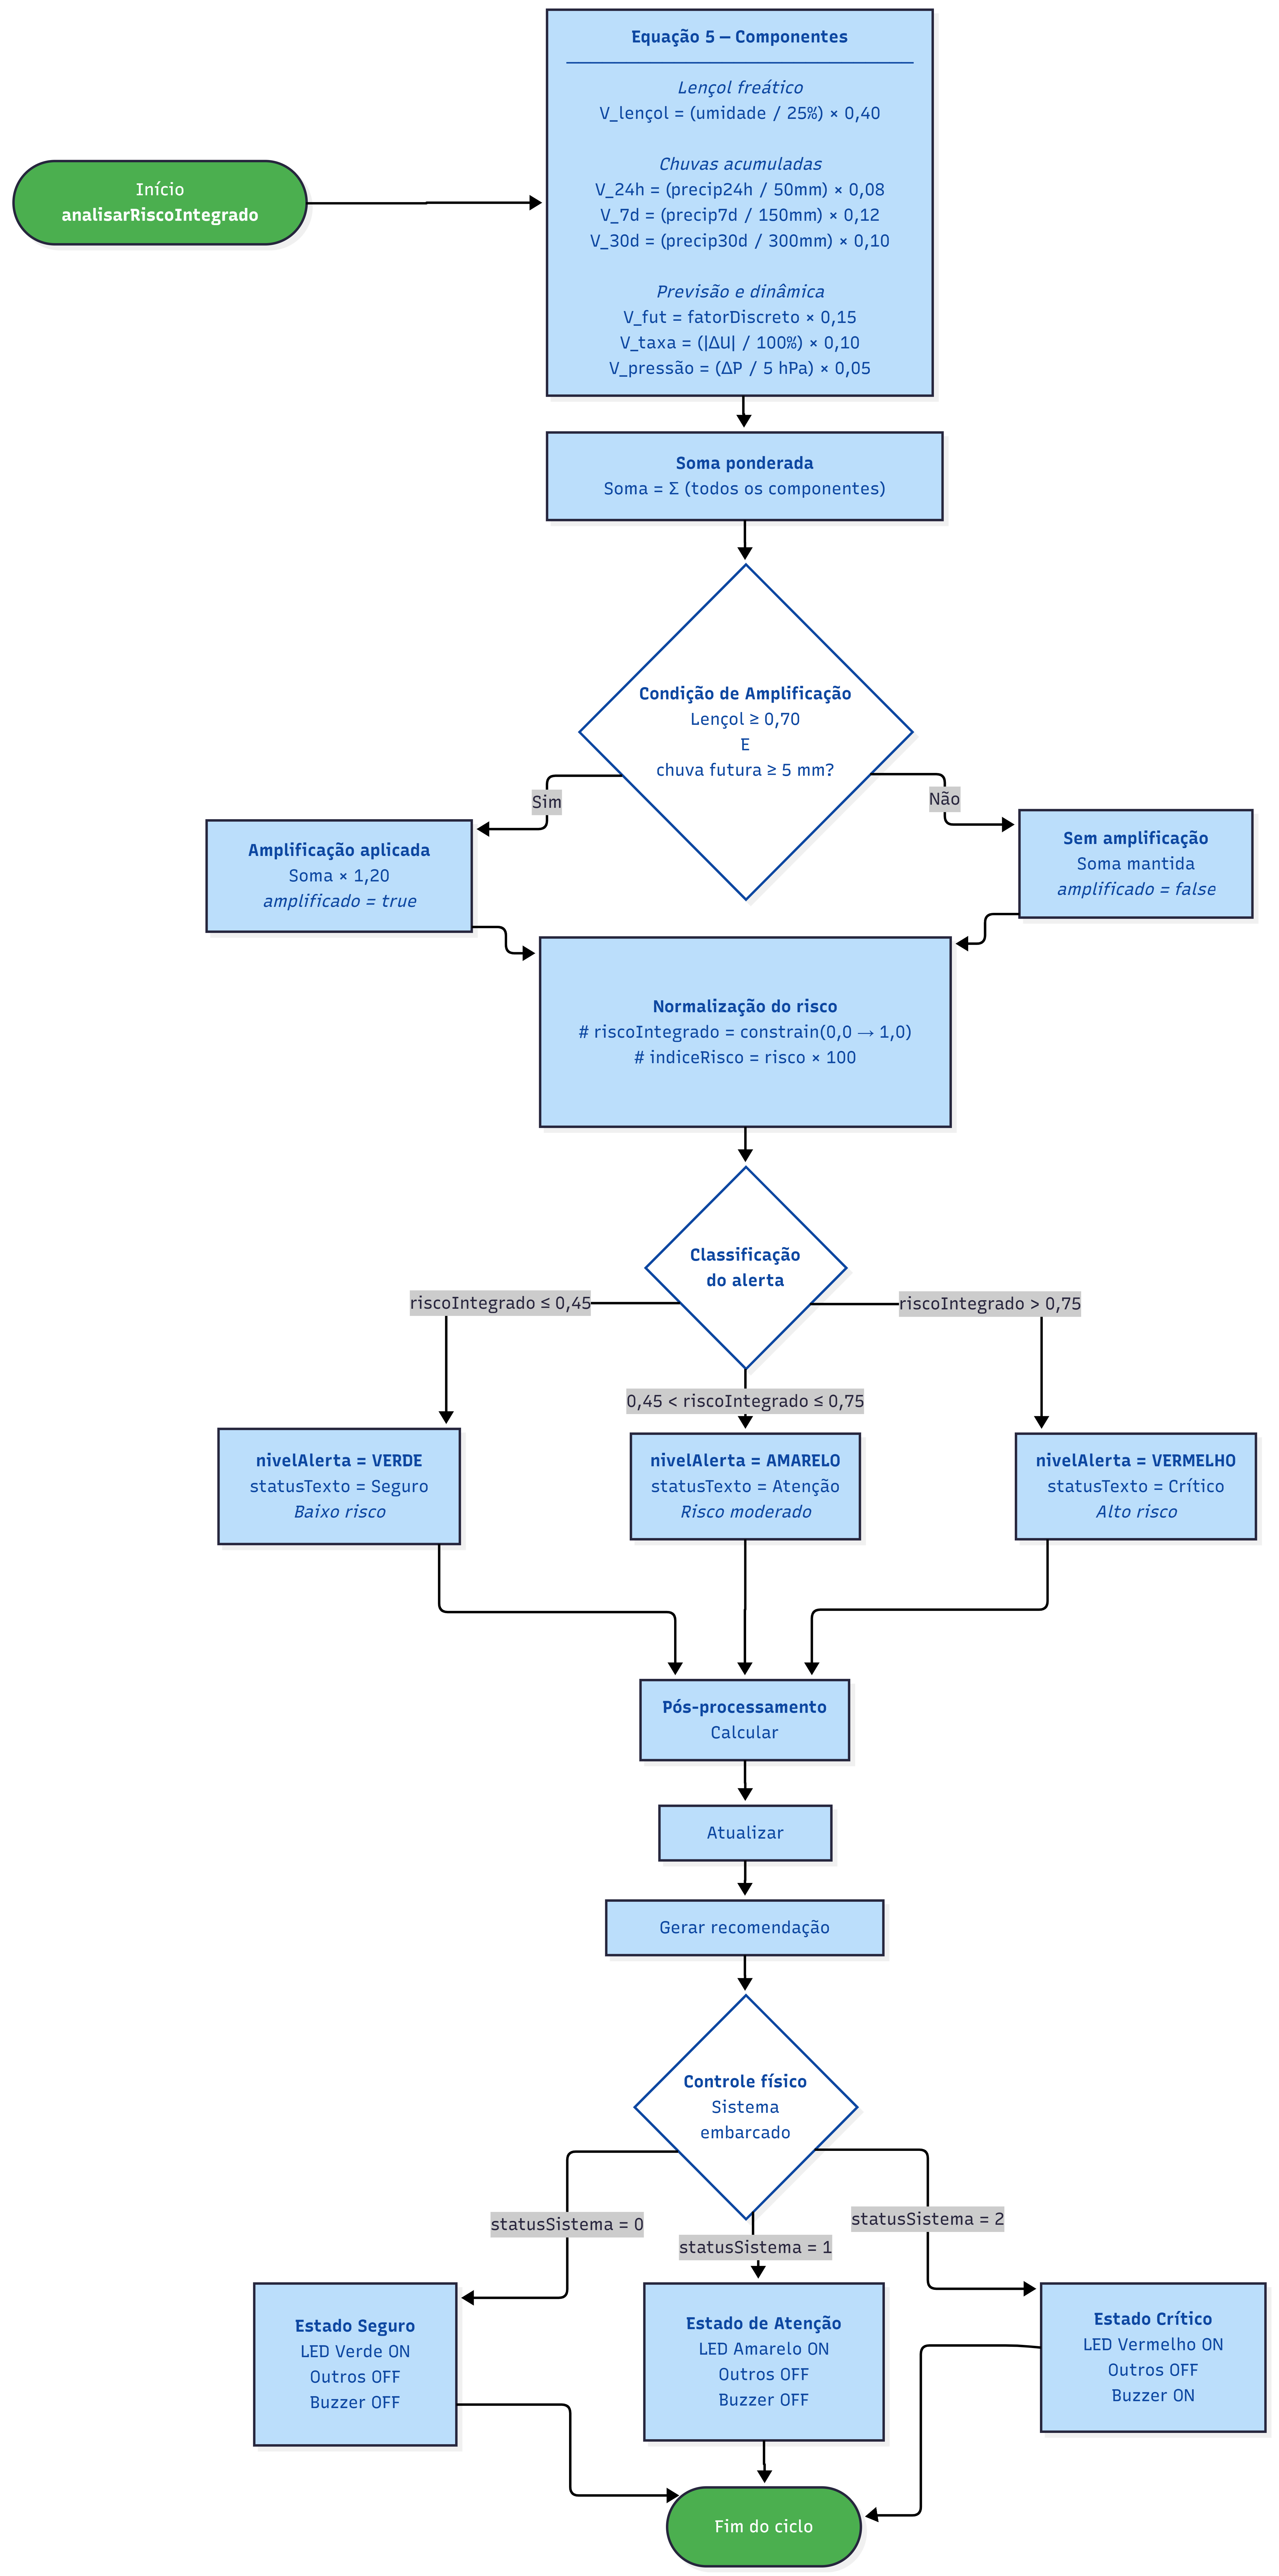
\includegraphics[width=0.75\textwidth]
    {figures/cap4_fluxograma_f2_ciclo_analise_risco.png}
\caption{Fluxograma do ciclo de análise de risco integrado}
\label{fig:fluxograma_risco}
\fonte{Elaborado pela autora.}
\end{figure}

O ciclo tem início com o cálculo dos sete componentes da
Equação~\ref{eq:frisco}. Cada componente é obtido de forma
independente a partir das estruturas de dados globais já
preenchidas pelos subsistemas de coleta: $V_{len}$ utiliza a
leitura mais recente do higrômetro; $V_{ch.24h}$, $V_{ch.7d}$ e
$V_{ch.30d}$ utilizam os acumulados pluviométricos obtidos da API
BNDMET/DECEA via fenômeno I006; $V_{ch.fut}$ é derivado da
classificação da previsão de precipitação das próximas 24 horas
obtida via \textit{endpoint} \texttt{/forecast} da API
OpenWeatherMap; $V_{taxa}$ é calculado sobre o \textit{buffer}
circular das dez últimas leituras de umidade; e $V_{press\~ao}$ é
obtido a partir da queda de pressão atmosférica registrada na
janela de três horas. Os pesos aplicados a cada componente somam
exatamente 1,00, de forma que o fator de risco integrado
$F_{risco}$ é adimensional e naturalmente limitado ao intervalo
$[0;\,1]$ em condições normais.

Após a soma dos sete componentes, o sistema avalia a condição de
amplificação. O mecanismo é ativado quando dois critérios são
satisfeitos simultaneamente: o $F_{len\c{c}ol}$ calculado para a
leitura atual atinge ou supera 0,70 — o que equivale a uma umidade
do solo igual ou superior a 17,5\% — e a precipitação prevista
para as próximas 24 horas é igual ou superior a 5\,mm, classe
mínima ``Moderada'' na tabela de intensidade pluviométrica
\cite{sistemaalertario2025}. Quando ambas as condições estão
presentes, a soma dos componentes é multiplicada por 1,20, elevando
o fator de risco em 20\%. A justificativa para esse mecanismo reside
na combinação de solo já próximo da saturação com previsão de chuva
iminente: isoladamente, cada condição pode não ser suficiente para
elevar o risco à faixa crítica; conjuntamente, aumentam
significativamente a probabilidade de rompimento
\cite{robertson2019feijaoson2019}. O resultado final é limitado ao
intervalo $[0;\,1]$ pela função \texttt{constrain}, evitando que
amplificações extremas produzam valores fora da escala do modelo.

A classificação do nível de alerta é realizada em seguida, com base
em três faixas definidas na Tabela~5 do trabalho: fator de risco
igual ou inferior a 0,45 corresponde ao nível VERDE (\textit{status}
``SEGURO''); acima de 0,45 e até 0,75, ao nível AMARELO
(\textit{status} ``ATENÇÃO''); acima de 0,75, ao nível VERMELHO
(\textit{status} ``CRÍTICO''). Os limiares foram escolhidos de forma
a manter o nível VERDE associado a situações de baixa combinação de
fatores e o VERMELHO reservado a cenários de risco elevado, com a
faixa AMARELO funcionando como zona de vigilância ativa.

Concluída a classificação, o ciclo executa em sequência três
subprocessos encadeados: o cálculo do índice de confiabilidade da
análise, a atualização do histórico interno de risco e a geração da
mensagem de recomendação operacional. Por fim, a função
\texttt{controlarSistemaFisico()} traduz o nível de alerta em ações
concretas de hardware: no nível VERDE, o LED verde é acionado e o
\textit{buzzer} permanece em silêncio; no nível AMARELO, o LED
amarelo é acionado, também sem acionamento sonoro; no nível VERMELHO,
o LED vermelho é acionado e o \textit{buzzer} passa ao estado ativo,
emitindo sinal intermitente com frequência proporcional ao índice de
risco — 2.000\,Hz para índice entre 80\% e 84\%, 2.200\,Hz entre
85\% e 89\%, e 2.400\,Hz para índice igual ou superior a 90\%. Vale
destacar que \texttt{controlarSistemaFisico()} contém uma guarda
explícita para o caso de ruptura: quando a umidade do solo está
acima de 30\%, o controle de hardware já foi realizado diretamente
por \texttt{acionarRuptura()} e a função retorna sem executar
qualquer ação adicional, garantindo que o LED vermelho e o
\textit{buzzer} de ruptura não sejam inadvertidamente desligados
durante o ciclo seguinte.

% -------------------------------------------------------------
\subsubsubsection{Fluxograma do Protocolo de Ruptura e Desescalada}
\label{subsubsec:fluxograma-ruptura}
% -------------------------------------------------------------

A Figura~\ref{fig:fluxograma_ruptura} apresenta o fluxograma do
protocolo de ruptura, executado a cada leitura do sensor de umidade
do solo. Este protocolo opera em paralelo ao ciclo de análise de
risco descrito na Seção~\ref{subsubsec:fluxograma-risco} e tem
precedência sobre ele: sempre que a condição de ruptura é detectada,
o mecanismo de análise ponderada é integralmente substituído por um
acionamento direto de emergência.

\begin{figure}[htb]
\centering
\includegraphics[width=0.95\textwidth]
    {figures/cap4_fluxograma_f3_protocolo_ruptura.png}
\caption{Fluxograma do protocolo de ruptura e desescalada}
\label{fig:fluxograma_ruptura}
\fonte{Elaborado pela autora.}
\end{figure}

O fluxo tem início com a verificação do limiar de ruptura: se a
umidade do solo lida pelo higrômetro é igual ou superior a 30\%,
a função \texttt{acionarRuptura()} é chamada imediatamente. Esta
função não executa a equação de risco ponderada — ao contrário, ela
força diretamente os valores de emergência: o fator de risco
integrado é fixado em 1,0, o índice de risco em 100\%, o nível de
alerta em VERMELHO e o campo \texttt{statusTexto} em
``\textsc{ruptura}''. O componente $V_{len\c{c}ol}$ é fixado no seu
valor máximo de 0,40, correspondente à saturação completa do fator
do lençol freático; o componente $V_{taxa}$ é recalculado com os
dados reais do \textit{buffer} circular naquele instante, garantindo
que a velocidade de saturação seja auditável mesmo durante a ruptura.
O mecanismo de amplificação não é aplicado — a ruptura já representa
o estado crítico máximo do modelo. Em seguida, o índice de
confiabilidade da análise é forçado para 100\% com o campo
\texttt{estado\_especial = "RUPTURA"}, refletindo que, neste estado,
o sensor físico confirma a condição de emergência diretamente, sem
dependência das APIs externas. Por fim, o hardware é acionado de
forma imediata — sem aguardar o próximo ciclo do
\texttt{loop()} —: o LED vermelho é ligado e o \textit{buzzer} emite
sinal contínuo na frequência de 2.400\,Hz.

A mesma verificação de ruptura está presente na função
\texttt{setup()}, executada uma única vez ao energizar o dispositivo.
Caso a umidade já esteja acima de 30\% no instante da inicialização
— cenário que pode ocorrer se o dispositivo for religado após um
evento crítico —, o protocolo é acionado antes de qualquer coleta
de dados meteorológicos ou análise de risco, garantindo que o
sistema entre em estado de emergência imediatamente após o
\textit{boot}.

Quando a umidade retorna abaixo de 30\%, o sistema não retoma a
análise normal de imediato. O fluxograma mostra que, se o
\texttt{statusTexto} ainda é ``\textsc{ruptura}'' mas a leitura
atual já está abaixo do limiar, o sistema entra na janela de
desescalada (\textit{cooldown}). A cada nova leitura segura, um
contador interno é incrementado e a variável
\texttt{aguardandoResetRuptura} é marcada como verdadeira — o que
faz com que os registros enviados ao \textit{backend} durante esse
período carreguem a indicação de ``\textsc{retorno de ruptura}'' no
campo \texttt{dadosBrutos}, permitindo que o painel \textit{web}
exiba uma mensagem diferenciada ao operador. Somente após três
leituras consecutivas com umidade abaixo do limiar o contador é
zerado, a \textit{flag} \texttt{aguardandoResetRuptura} é desativada
e a função \texttt{analisarRiscoIntegrado()} é chamada, retomando o
ciclo ponderado normal.

A exigência de três confirmações consecutivas antes de encerrar o
estado de ruptura decorre da necessidade de garantir que a queda de
umidade não seja transitória — provocada, por exemplo, por uma
oscilação do sensor ou por um movimento de solo que redistribua
momentaneamente a umidade na vizinhança da sonda. Três leituras
consecutivas abaixo do limiar, nos intervalos adaptativos do nível
VERMELHO (5 segundos entre cada leitura), correspondem a uma janela
mínima de 10 segundos de estabilidade antes da reabertura do ciclo
analítico, conferindo robustez ao critério de desescalada.

% -------------------------------------------------------------
\subsubsubsection{Fluxograma do Loop Principal de Orquestração}
\label{subsubsec:fluxograma-loop}
% -------------------------------------------------------------

A Figura~\ref{fig:fluxograma_loop} apresenta o fluxograma do
\textit{loop} principal do \textit{firmware}, função executada
continuamente pelo microcontrolador após a conclusão do
\texttt{setup()}. O \textit{loop} não executa todos os subsistemas
a cada iteração: a orquestração é baseada em cinco temporizadores
independentes, cada um comparando o instante atual obtido por
\texttt{millis()} com o instante do último disparo de cada
subsistema. Esta abordagem é característica de sistemas embarcados de baixo
custo, nos quais a ausência de um sistema operacional dedicado
exige que o próprio programa controle a ordem e o momento de
execução de cada tarefa \cite{sommerville2011engenharia}.

\begin{figure}[htb]
\centering
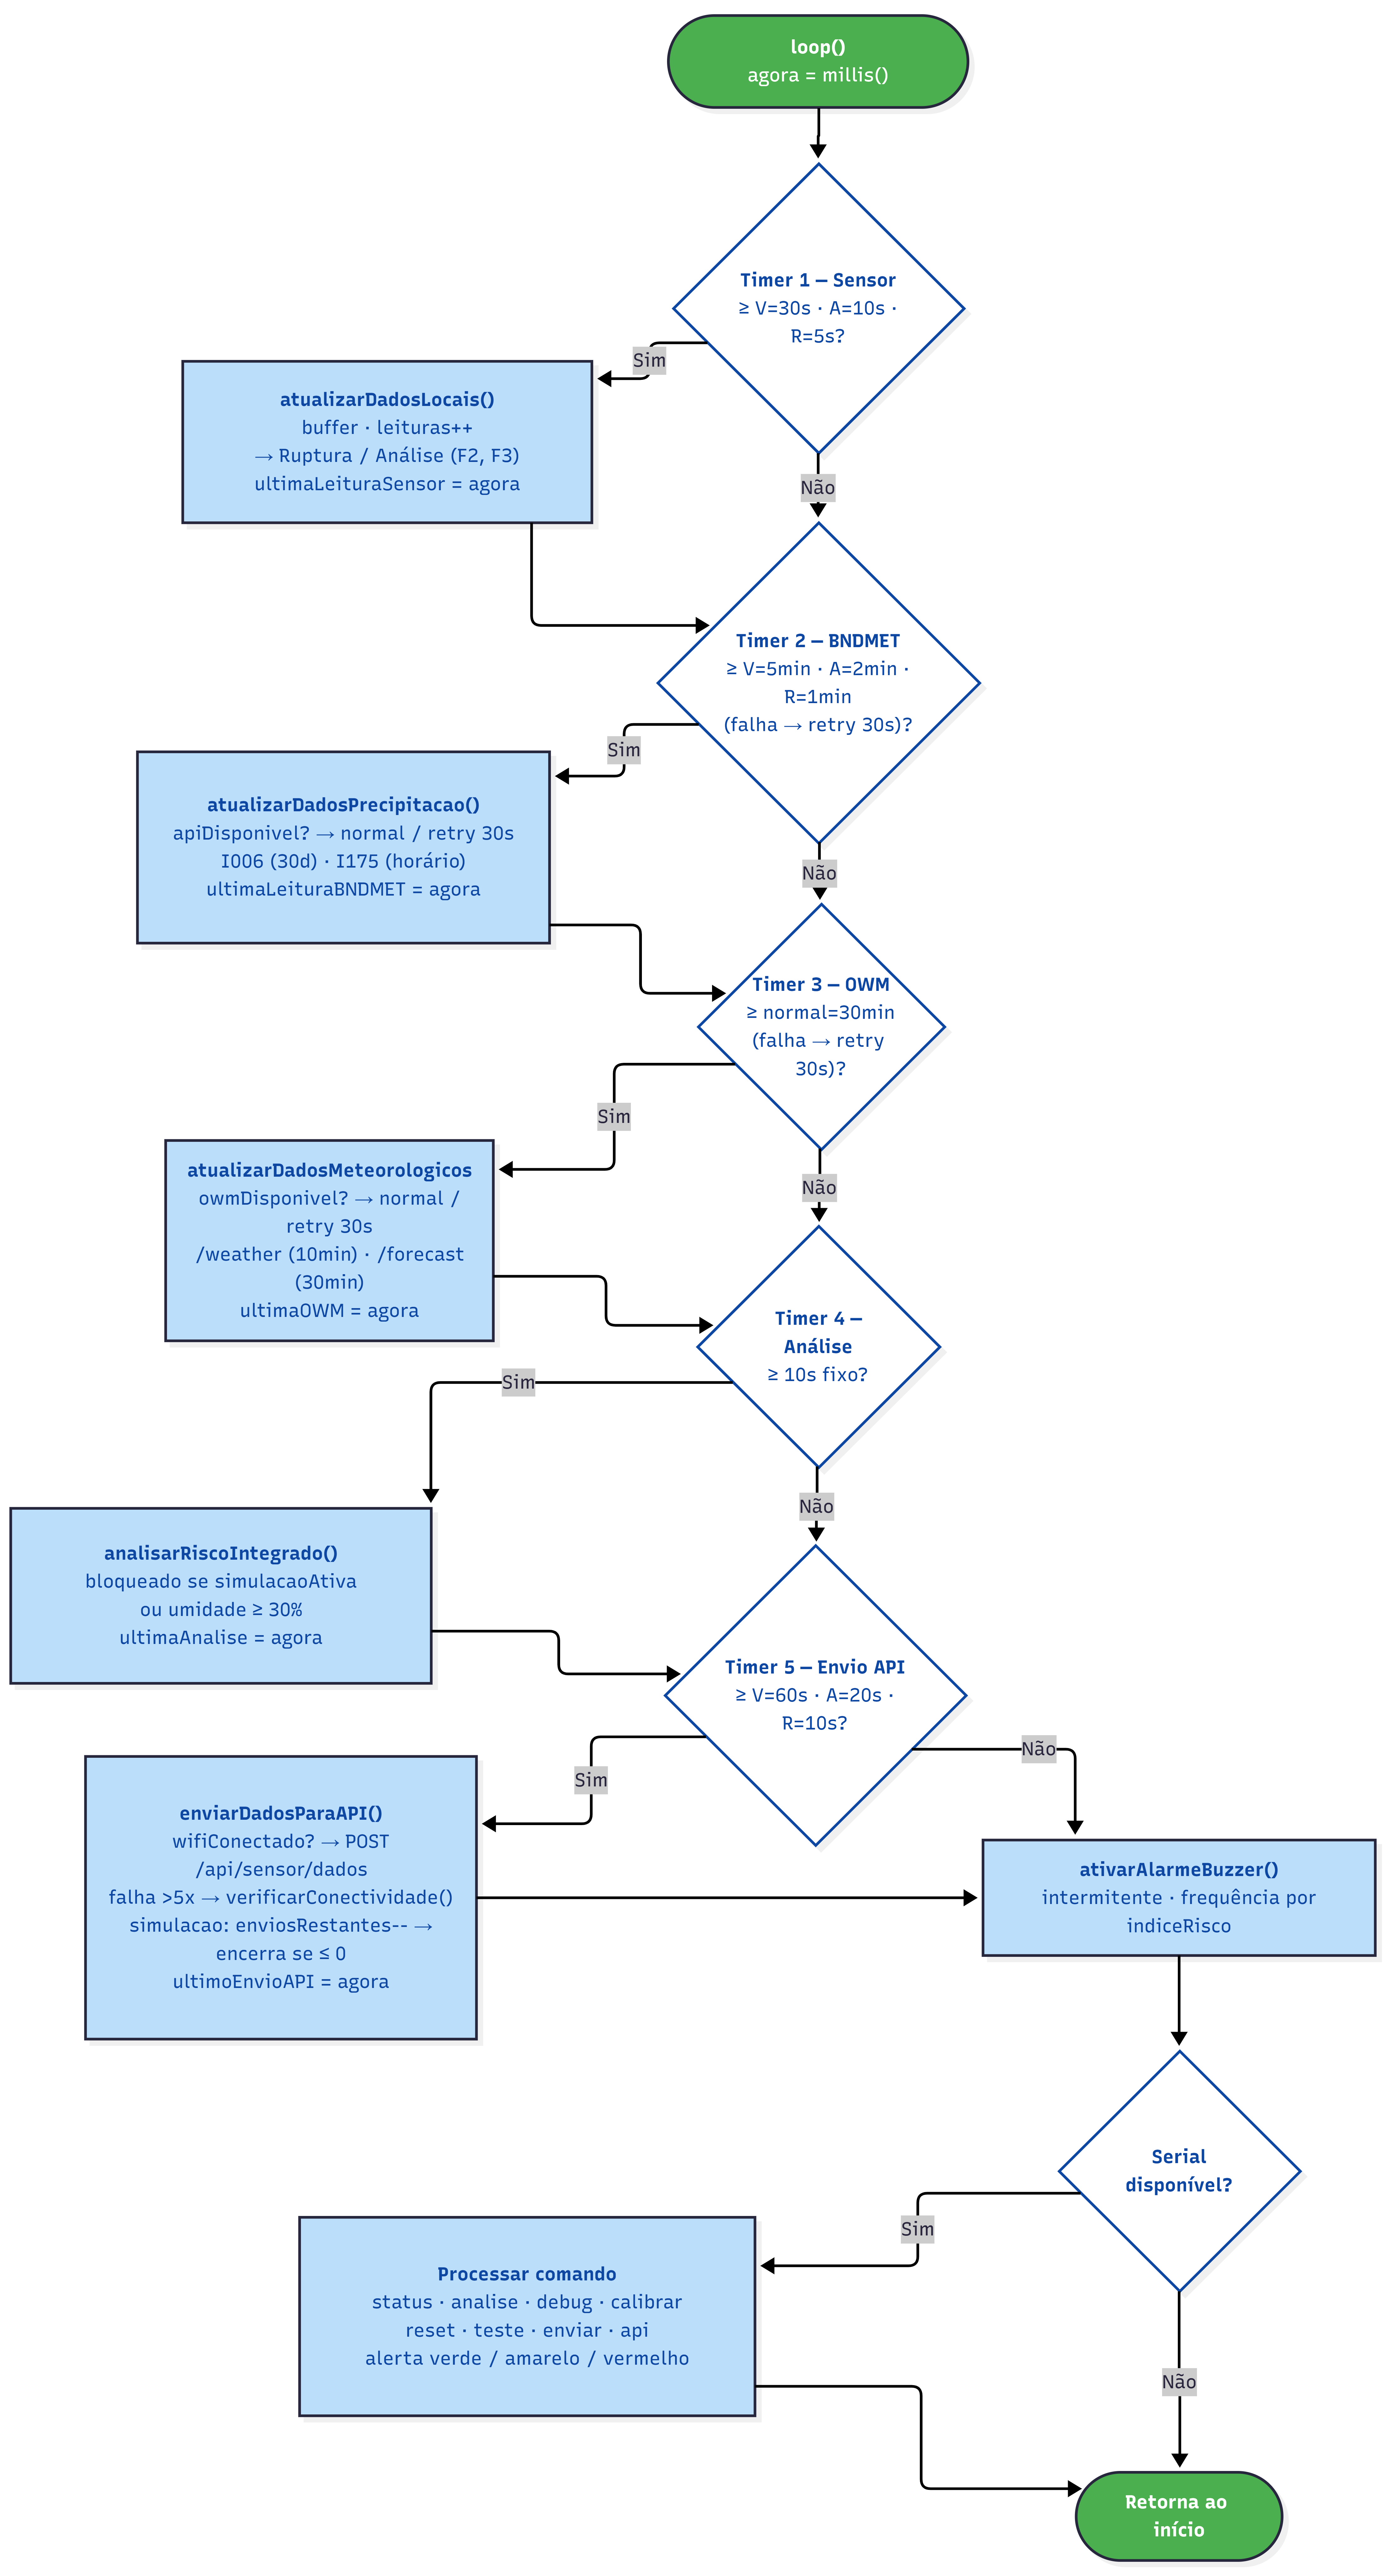
\includegraphics[width=0.80\textwidth]
    {figures/cap4_fluxograma_f1_loop_principal.png}
\caption{Fluxograma do \textit{loop} principal de orquestração do
\textit{firmware}}
\label{fig:fluxograma_loop}
\fonte{Elaborado pela autora.}
\end{figure}

O primeiro temporizador controla a leitura do higrômetro. O
intervalo entre leituras é adaptativo e determinado pelo nível de
alerta vigente: 30 segundos no nível VERDE, 10 segundos no nível
AMARELO e 5 segundos no nível VERMELHO. Quando o timer dispara,
o firmware lê o valor ADC do pino A0, mapeia o resultado para o
intervalo de 0\% a 100\% de umidade, atualiza o \textit{buffer}
circular de dez posições utilizado no cálculo da taxa de variação
e incrementa o contador total de leituras. A decisão de ruptura e
o ciclo de análise de risco, acionados em seguida conforme as
condições descritas nos Fluxogramas~\ref{fig:fluxograma_risco}
e~\ref{fig:fluxograma_ruptura}, integram este mesmo bloco de
leitura do sensor.

O segundo temporizador controla a consulta à API BNDMET/DECEA.
Em condições normais, o intervalo é adaptativo por nível de alerta:
5 minutos no nível VERDE, 2 minutos no nível AMARELO e 1 minuto
no nível VERMELHO. Quando a última consulta à API terminou em
falha — indicado pelo campo \texttt{apiDisponivel = false} —, o
intervalo é substituído por um valor fixo de 30 segundos,
independentemente do nível de alerta. Esse mecanismo de
\textit{retry} acelerado garante que os dados pluviométricos
sejam recuperados o mais rapidamente possível após uma falha
transitória de rede ou de indisponibilidade da API, sem
sobrecarregar o servidor em condições de falha persistente.

O terceiro temporizador controla as consultas à API OpenWeatherMap.
Diferentemente do sensor e do BNDMET, o intervalo do OWM não varia
com o nível de alerta: o \textit{endpoint} \texttt{/forecast} é
consultado a cada 30 minutos fixos, e o \texttt{/weather} a cada
10 minutos, ambos acionados pela mesma função
\texttt{atualizarDadosMeteorologicos()}. Quando a API ainda não foi
consultada com sucesso desde o \textit{boot} — identificado pelo
campo \texttt{timestamp = 0} da estrutura \texttt{DadosMeteorologicos}
—, o mesmo intervalo de \textit{retry} de 30 segundos é aplicado
até que a primeira resposta válida seja obtida.

O quarto temporizador executa a análise de risco integrado a cada
10 segundos fixos. Antes de chamar \texttt{analisarRiscoIntegrado()},
duas condições de bloqueio são verificadas: se uma simulação de nível
está ativa (\texttt{simulacaoAtiva = true}), a análise é suspensa
para preservar os valores injetados manualmente; e se a umidade do
solo está acima de 30\%, a análise também é bloqueada, pois o
estado de ruptura já está sendo gerenciado pelo protocolo descrito
no Fluxograma~\ref{fig:fluxograma_ruptura}. Ambas as guardas evitam
que o ciclo analítico sobrescreva estados críticos ou de teste
indevidamente.

O quinto temporizador controla o envio dos dados ao
\textit{backend} local. O intervalo de envio é adaptativo por nível
de alerta: 60 segundos no nível VERDE, 20 segundos no nível
AMARELO e 10 segundos no nível VERMELHO. O envio só ocorre se a
conexão Wi-Fi está estabelecida. Em caso de falha no envio com mais
de cinco tentativas consecutivas acumuladas, o sistema chama
\texttt{verificarConectividade()} para tentar a reconexão. Quando
uma simulação de nível está ativa, cada envio bem-sucedido decrementa
o contador \texttt{simulacaoEnviosRestantes}; ao atingir zero, a
simulação é encerrada automaticamente — as \textit{flags}
\texttt{simulacaoAtiva} e \texttt{modoManual} são desativadas, o
\textit{buzzer} é silenciado e o \textit{firmware} retorna ao
modo de operação automático.

Após os cinco temporizadores, o \textit{loop} chama
\texttt{ativarAlarmeBuzzer()} — função que gerencia o padrão
intermitente do \textit{buzzer} quando \texttt{buzzerAtivo = true},
variando a frequência e o intervalo de pulsação conforme o índice de
risco. Por fim, o laço verifica se há bytes disponíveis na porta
Serial e, se houver, lê e processa o comando recebido. Os comandos
disponíveis permitem consultar o status do sistema, forçar análises
manuais, executar calibração do sensor e acionar simulações de
nível para fins de teste e demonstração.

% -------------------------------------------------------------
\subsubsubsection{Fluxograma do Cálculo do Índice de Confiabilidade}
\label{subsubsec:fluxograma-confiabilidade}
% -------------------------------------------------------------

A Figura~\ref{fig:fluxograma_confiabilidade} apresenta o fluxograma
do cálculo do índice de confiabilidade da análise, executado ao
final de cada ciclo de \texttt{analisarRiscoIntegrado()} e também
dentro de \texttt{acionarRuptura()}, garantindo que todo registro
persistido no banco de dados carregue um percentual de confiabilidade
auditável. O índice expressa o grau de completude e atualidade dos
dados que alimentaram o cálculo de risco naquele ciclo específico,
variando de 0\% a 100\%.

\begin{figure}[htb]
\centering
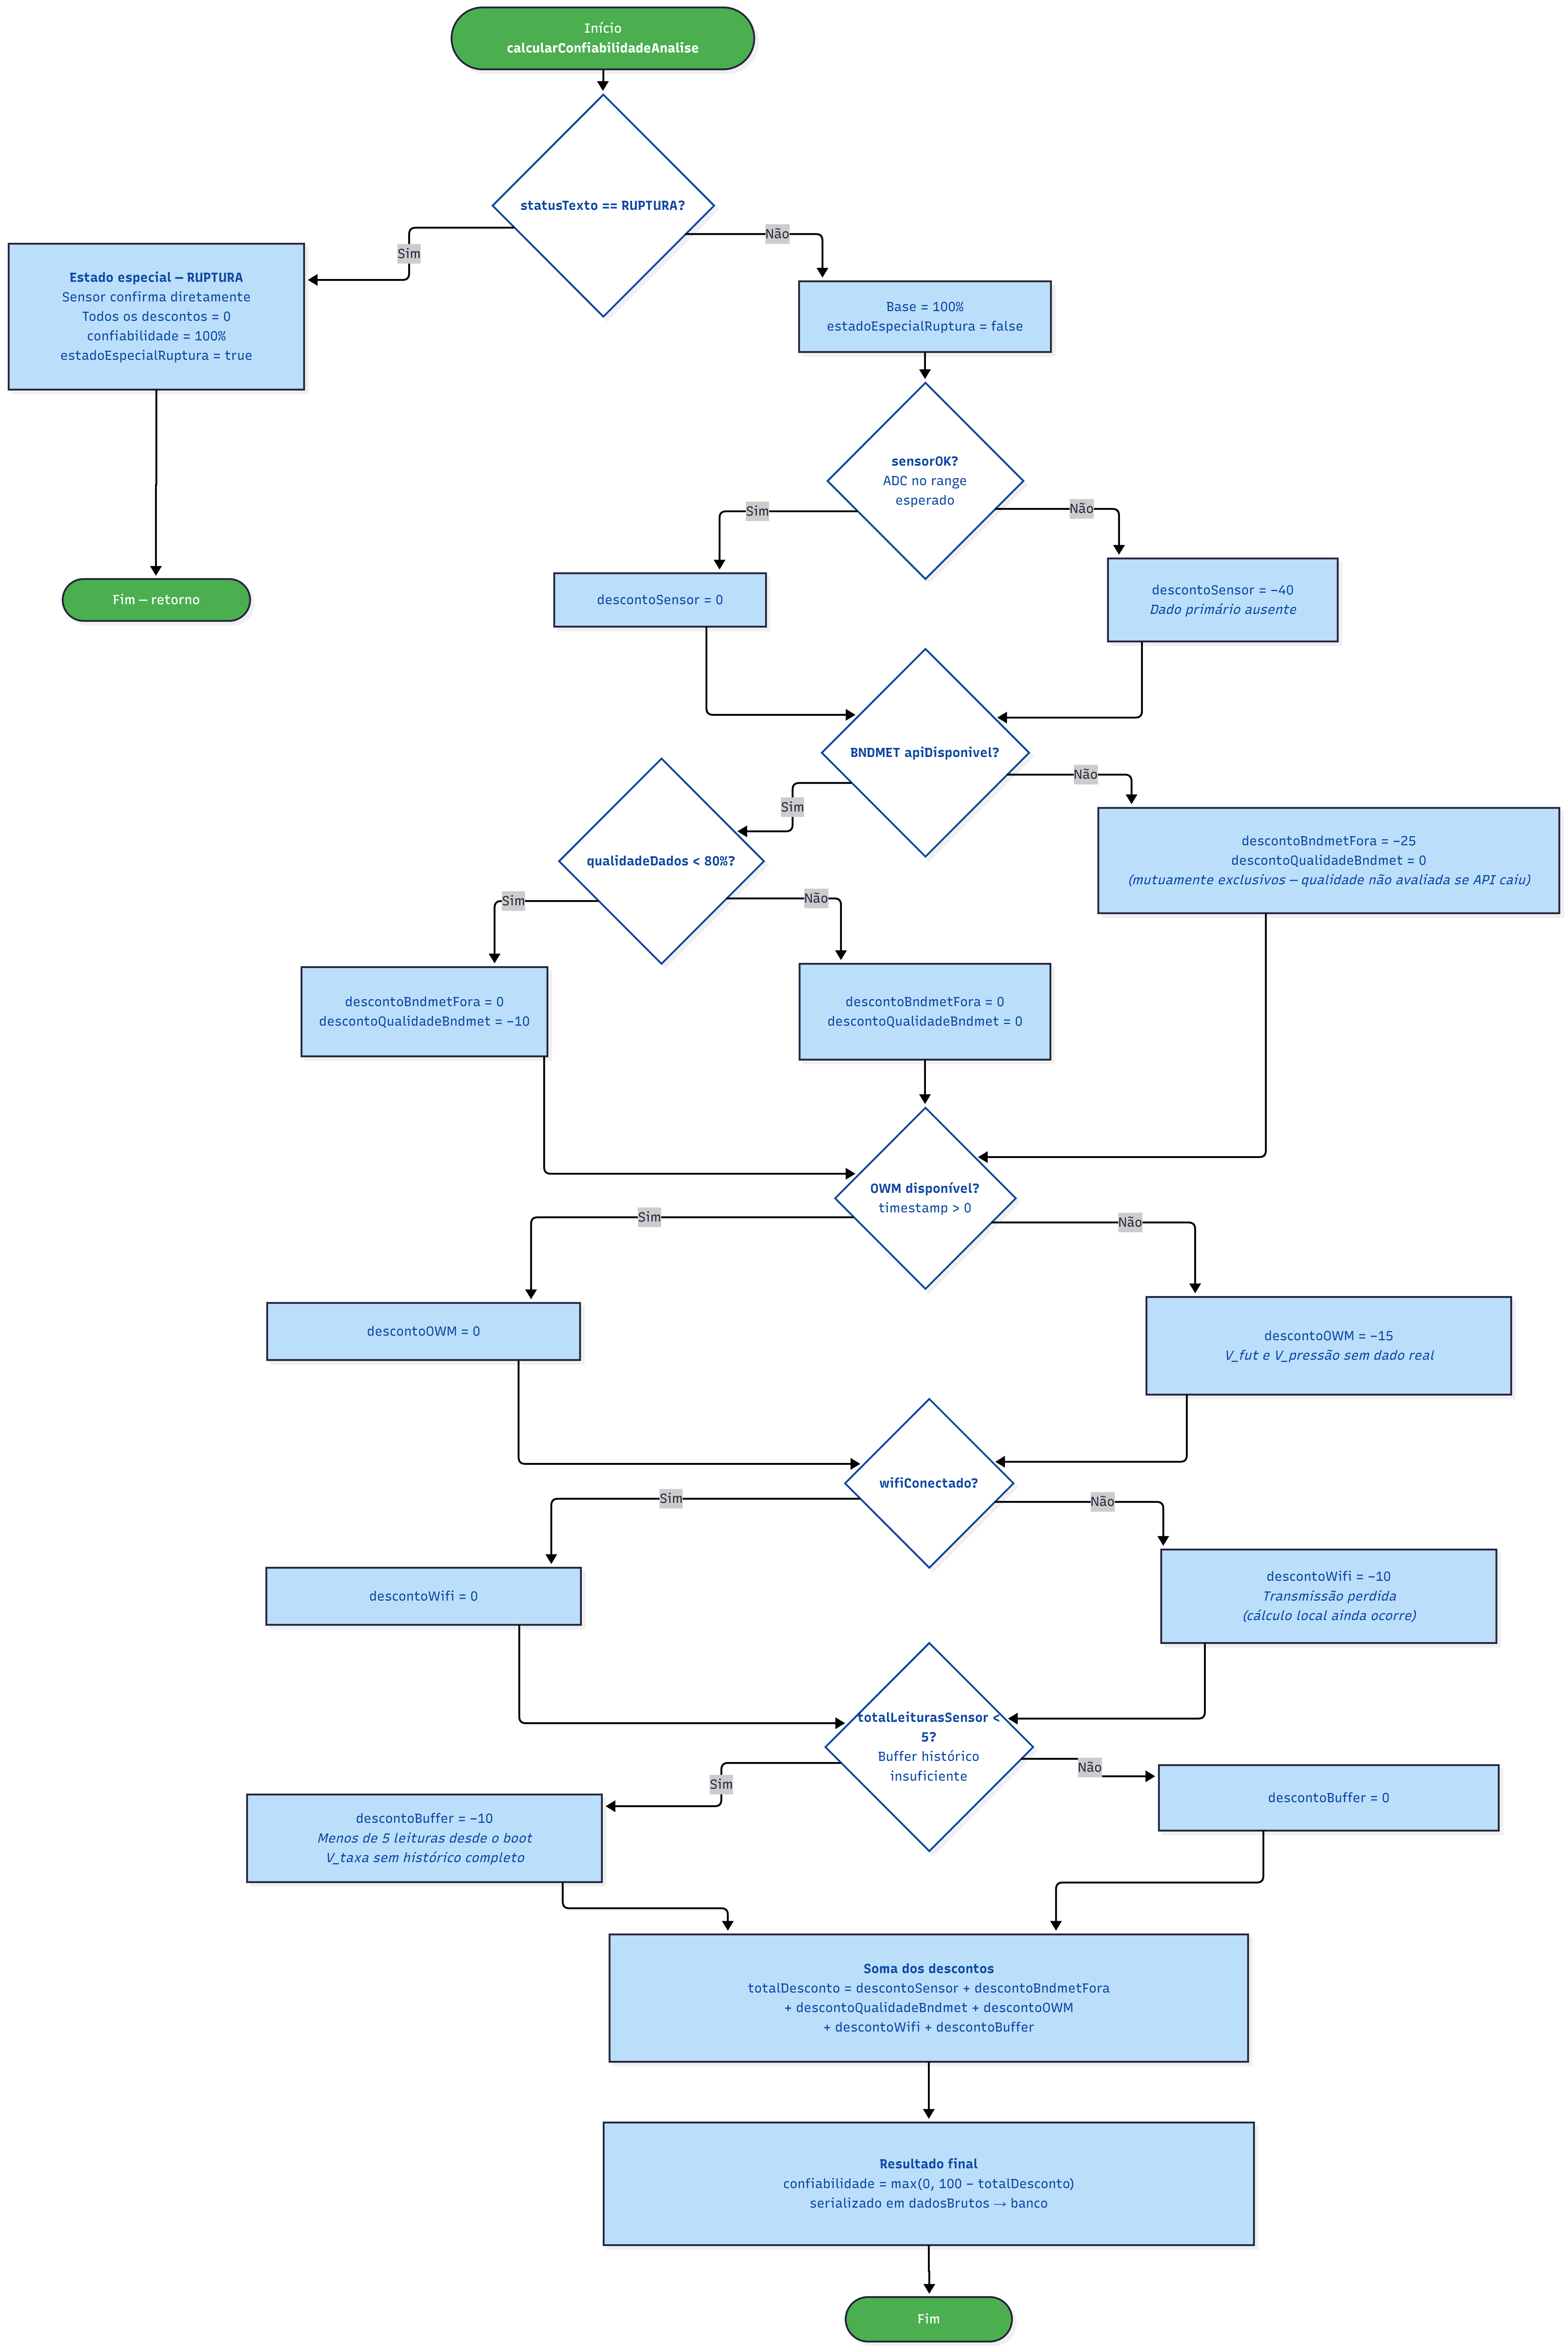
\includegraphics[width=0.95\textwidth]
    {figures/cap4_fluxograma_f4_confiabilidade.png}
\caption{Fluxograma do cálculo do índice de confiabilidade da análise}
\label{fig:fluxograma_confiabilidade}
\fonte{Elaborado pela autora.}
\end{figure}

O fluxo se divide em dois caminhos desde o primeiro nó de decisão.
Quando o campo \texttt{statusTexto} da estrutura \texttt{AnaliseRisco}
contém o valor ``\textsc{ruptura}'', o sistema entra no caminho de
estado especial: todos os descontos são zerados e a confiabilidade é
fixada em 100\%, independentemente de qualquer falha de sensor ou
API que possa estar presente naquele instante. A justificativa é que,
no estado de ruptura, o sensor físico confirma diretamente a condição
crítica por meio da leitura de umidade acima de 30\% — não há
ambiguidade sobre o estado do sistema e a informação primária está
disponível com máxima certeza. O campo \texttt{estado\_especial}
é preenchido com ``\textsc{ruptura}'' no objeto
\texttt{confiabilidade\_detalhes} serializado em \texttt{dadosBrutos},
permitindo que o painel \textit{web} exiba a indicação correspondente
ao operador.

Quando o sistema não está em estado de ruptura, o cálculo segue o
caminho normal por descontos cumulativos, partindo de uma base de
100\% e subtraindo percentuais específicos para cada fonte de
degradação identificada. As cinco avaliações são independentes entre
si, com exceção de uma exclusividade mútua entre dois descontos
relacionados ao BNDMET, descrita a seguir.

O primeiro desconto avalia o sensor físico: se o valor ADC lido no
pino A0 está fora do intervalo esperado — indicado pelo campo
\texttt{sensorOK = false} —, aplica-se um desconto de 40 pontos.
Trata-se do maior desconto individual do modelo, refletindo que a
umidade do solo é o dado primário do sistema e sua ausência
compromete o componente de maior peso da equação de risco.

A segunda avaliação trata os dados pluviométricos da API
BNDMET/DECEA com dois descontos mutuamente exclusivos. Se a API
estava indisponível na última consulta (\texttt{apiDisponivel =
false}), aplica-se um desconto de 25 pontos e o desconto de
qualidade é zerado — não faz sentido avaliar a qualidade dos dados
de uma API que não respondeu. Se a API respondeu mas a qualidade dos
dados retornados é inferior a 80\%, aplica-se um desconto de 10
pontos.

O terceiro desconto avalia a disponibilidade da API OpenWeatherMap:
quando o campo \texttt{timestamp} da estrutura
\texttt{DadosMeteorologicos} é zero — indicando que a API nunca
respondeu com sucesso desde o \textit{boot} ou que a última
tentativa falhou —, aplica-se um desconto de 15 pontos, pois os
componentes $V_{ch.fut}$ e $V_{press\~ao}$ não possuem dados reais
para o ciclo.

O quarto desconto avalia a conectividade Wi-Fi: quando a conexão
está inativa, aplica-se um desconto de 10 pontos. É importante
destacar que a desconexão Wi-Fi não impede o cálculo de risco — o
\textit{firmware} continua operando com os últimos dados disponíveis
em memória e acionando os indicadores físicos locais. O desconto
reflete apenas que a transmissão dos dados ao \textit{backend} está
comprometida, reduzindo a completude da análise do ponto de vista
do sistema como um todo.

O quinto e último desconto avalia o histórico do \textit{buffer}
circular de umidade: quando o contador total de leituras desde o
\textit{boot} é inferior a cinco (\texttt{totalLeiturasSensor < 5}),
aplica-se um desconto de 10 pontos, indicando que o componente
$V_{taxa}$ não dispõe de histórico suficiente para uma estimativa
confiável da velocidade de saturação do solo.

Ao final das cinco avaliações, os descontos são somados e
subtraídos da base de 100, com o resultado limitado a zero por
\texttt{max(0, 100 - totalDesconto)}, garantindo que o índice
nunca assuma valores negativos mesmo em cenários de múltiplas
falhas simultâneas. O resultado e o detalhamento individual de
cada desconto são armazenados na estrutura
\texttt{ConfiabilidadeDetalhes} e serializados no campo
\texttt{dadosBrutos} do \textit{payload} JSON enviado ao
\textit{backend}, onde são persistidos na coluna \texttt{dados\_brutos}
do tipo \texttt{jsonb} na tabela \texttt{leituras\_sensor}, tornando
cada decisão de confiabilidade auditável pelo painel \textit{web}.

% -------------------------------------------------------------
\subsubsection{Fluxograma de Recebimento e Persistência de Leitura}
\label{subsubsec:fluxograma-backend-sensor}
% -------------------------------------------------------------

A Figura~\ref{fig:fluxograma_backend_sensor} apresenta o fluxograma
do processo de recebimento, validação e persistência de leituras
do sensor, executado pelo \textit{backend} Node.js a cada requisição
\texttt{POST /api/sensor/dados} enviada pelo \textit{firmware} do
ESP8266.

\begin{figure}[htb]
\centering
\includegraphics[width=0.95\textwidth]
    {figures/cap4_fluxograma_f5_backend_sensor.png}
\caption{Fluxograma de recebimento e persistência de leitura no
\textit{backend}}
\label{fig:fluxograma_backend_sensor}
\fonte{Elaborado pela autora.}
\end{figure}

A rota \texttt{POST /api/sensor/dados} é a única rota do sistema
que não exige autenticação JWT — uma decisão deliberada de projeto,
pois o ESP8266 opera em rede local e não possui mecanismo nativo
de gestão de tokens com renovação periódica. A requisição chega ao
método \texttt{SensorController.receberDados()}, que realiza uma
validação inicial de estrutura: se o corpo da requisição estiver
ausente ou não for um objeto, o \textit{backend} retorna
imediatamente \texttt{HTTP 400} com mensagem de erro, sem invocar
a camada de serviço. Passada a validação, o processamento é
delegado ao método \texttt{SensorService.salvarDados()}.

Antes de persistir os dados, o serviço executa três normalizações
sobre campos críticos. O campo \texttt{sensorOk}, que indica se o
sensor está operacional, é forçado para \texttt{false} explícito
quando chega como \texttt{undefined} ou \texttt{null} — situação
que ocorre quando o valor ADC lido pelo ESP8266 é 1024, indicando
sensor desconectado, e o campo é omitido do \textit{payload}. O
campo \texttt{amplificado} é avaliado por comparação estrita
(\texttt{=== true}), evitando que valores \textit{truthy} não
booleanos sejam gravados como \texttt{true} na coluna correspondente.
O campo \texttt{modoManual} recebe tratamento diferenciado: quando
enviado pelo \textit{firmware} em operação automática, carrega o
valor \texttt{false}; durante a simulação de nível via Serial, o
\textit{firmware} seta \texttt{modoManual = true} explicitamente
antes do envio, e o campo chega ao \textit{backend} como booleano
\texttt{true}; quando a requisição é enviada manualmente por
ferramentas como Postman ou \textit{curl}, o campo é omitido e o
serviço interpreta sua ausência como \texttt{true}, sinalizando ao
banco que aquela leitura não foi gerada pelo ciclo automático.

A persistência é realizada via Prisma ORM com o método
\texttt{prisma.leiturasSensor.create()}, que insere um registro
com aproximadamente 40 colunas na tabela \texttt{leituras\_sensor},
gerenciada pelo TimescaleDB como hipertabela particionada por
\texttt{timestamp}. O campo \texttt{dadosBrutos}, de tipo
\texttt{jsonb} no PostgreSQL, recebe o objeto de diagnóstico do
\textit{firmware} sem mapeamento de colunas — isso inclui os
detalhes individuais de confiabilidade, o indicador de janela de
\textit{cooldown} de ruptura e o sinalizador de inicialização do
BNDMET, todos acessíveis por consultas ao campo \texttt{jsonb}
diretamente no banco ou via API.

Em caso de falha na persistência, o método lança uma exceção que
é capturada pelo \texttt{try-catch} do controlador, que retorna
\texttt{HTTP 500} ao ESP8266. Do lado do \textit{firmware}, a
ausência de HTTP 201 na resposta incrementa o contador
\texttt{tentativasEnvioAPI}, que pode acionar a verificação de
conectividade após cinco falhas consecutivas.

Após a persistência bem-sucedida, o serviço classifica o nível
do log de operação com base em dois campos: \texttt{nivelAlerta}
e \texttt{riscoIntegrado}. Registros com \texttt{riscoIntegrado}
igual ou superior a 1,0 e \texttt{nivelAlerta = VERMELHO} são
tratados como \textsc{critical} quando a ruptura está ativa, e
como \textsc{warning} quando o sistema está na janela de
desescalada (\texttt{aguardandoResetRuptura = true}), separando
os dois estados na tabela de logs para facilitar a análise
posterior. Registros com nível VERDE são classificados como
\textsc{info}, e os demais como \textsc{warning} ou
\textsc{critical} conforme os limiares da equação de risco.
Adicionalmente, registros gerados antes da sincronização NTP
--- identificados pelo campo \texttt{bndmet\_inicializado = false}
dentro de \texttt{dadosBrutos} --- produzem um aviso no console
do servidor, sinalizando que os dados pluviométricos daquele
ciclo não refletem uma consulta real à API BNDMET.

O log de operação é persistido na tabela \texttt{logs\_sistema}
com o campo \texttt{dadosExtras} em \texttt{jsonb}, contendo o
identificador da leitura associada, o fator de risco, o nível de
alerta, o índice de confiabilidade, o indicador de amplificação
e o status da API BNDMET naquele ciclo. Por fim, o controlador
retorna \texttt{HTTP 201} ao ESP8266 com o corpo
\texttt{\{"success": true\}}, encerrando o ciclo de envio do
\textit{firmware}.

% -------------------------------------------------------------
\subsubsubsection{Fluxograma de Autenticação JWT e Validação de Sessão}
\label{subsubsec:fluxograma-auth}
% -------------------------------------------------------------

A Figura~\ref{fig:fluxograma_auth} apresenta o fluxograma do
mecanismo de autenticação do sistema, composto por três fluxos
complementares: o login, que cria a sessão; a validação de token
pelo \textit{middleware}, que protege as rotas autenticadas; e o
\textit{logout}, que invalida a sessão no banco de dados.

\begin{figure}[htb]
\centering
\includegraphics[width=0.95\textwidth]
    {figures/cap4_fluxograma_f6_autenticacao_jwt.png}
\caption{Fluxograma de autenticação JWT e validação de sessão}
\label{fig:fluxograma_auth}
\fonte{Elaborado pela autora.}
\end{figure}

O fluxo de login tem início com a validação dos campos de entrada
pelo \textit{middleware} \texttt{express-validator}: se o corpo da
requisição contiver campos ausentes ou com formato inválido, o
\textit{backend} retorna \texttt{HTTP 400} antes de qualquer consulta
ao banco. Passada essa validação, o serviço busca na tabela
\texttt{usuarios\_admin} um registro cujo e-mail, normalizado para
letras minúsculas, coincida com o fornecido e cujo campo
\texttt{ativo} seja verdadeiro. A normalização para minúsculas
evita falhas de autenticação por diferença de capitalização no
e-mail. Se nenhum registro for encontrado, ou se o \textit{hash}
bcrypt da senha fornecida não coincidir com o armazenado, o serviço
lança uma exceção genérica com a mensagem ``Credenciais
inválidas'' --- a mesma em ambos os casos, deliberadamente, para
não revelar ao requisitante se o e-mail existe no sistema.

Após a validação bem-sucedida das credenciais, o serviço gera um
token JWT assinado com a chave \texttt{JWT\_SECRET} e validade
configurada por \texttt{JWT\_EXPIRES\_IN}. O \textit{payload} do
token contém o identificador UUID do usuário, seu e-mail e seu
perfil (\texttt{admin} ou \texttt{super\_admin}). Em seguida, a
sessão é persistida na tabela \texttt{sessoes\_usuario} com o
token completo, o endereço IP, o agente de usuário e a data de
expiração calculada a partir do valor de \texttt{JWT\_EXPIRES\_IN}
--- suportando sufixos \texttt{h} (horas), \texttt{d} (dias) e
\texttt{m} (minutos). Por fim, o campo \texttt{ultimoLogin} do
administrador é atualizado e o token é retornado ao
\textit{frontend} junto com os dados do usuário e a data de
expiração da sessão.

O fluxo de validação de token é executado pelo
\textit{middleware} \texttt{verificarAutenticacao} a cada
requisição a uma rota protegida. A primeira verificação é
estrutural: o cabeçalho \texttt{Authorization} deve estar presente
e iniciar com o prefixo \texttt{Bearer} seguido de espaço; caso
contrário, a requisição é rejeitada imediatamente com
\texttt{HTTP 401} sem consulta ao banco. Em seguida, o token é
extraído e submetido a \texttt{jwt.verify()}, que valida a
assinatura criptográfica e verifica se o token não está expirado
por tempo --- esta verificação é inteiramente local, sem acesso ao
banco. Somente após a validação criptográfica bem-sucedida o
serviço consulta a tabela \texttt{sessoes\_usuario} com três
condições simultâneas: o token deve corresponder exatamente ao
registrado, o campo \texttt{ativo} da sessão deve ser verdadeiro
e a data de expiração deve ser posterior ao instante atual. Esta
dupla verificação --- criptográfica e no banco --- permite que
sessões sejam invalidadas explicitamente por \textit{logout} ou
por desativação do usuário, mesmo que o token JWT ainda não
tenha expirado por tempo. Se a sessão for encontrada e o usuário
estiver ativo, o objeto \texttt{req.user} é populado com os dados
do administrador e o \textit{middleware} chama \texttt{next()},
liberando a execução para o \textit{controller} correspondente.

O fluxo de \textit{logout} é o mais simples dos três: o
\textit{backend} extrai o token do cabeçalho de autorização ---
sem retornar erro se o cabeçalho estiver ausente --- e executa
\texttt{prisma.sessoesUsuario.updateMany()} para marcar
\texttt{ativo = false} em todos os registros com aquele token.
A deleção lógica preserva o histórico de sessões no banco para
fins de auditoria e, na próxima requisição com o mesmo token,
a consulta da etapa de validação não encontrará nenhuma sessão
ativa, resultando em \texttt{HTTP 401} imediato.

% -------------------------------------------------------------
\subsubsubsection{Fluxograma de Detecção de Status do Sensor no
\textit{Frontend}}
\label{subsubsec:fluxograma-status-sensor}
% -------------------------------------------------------------

A Figura~\ref{fig:fluxograma_status_sensor} apresenta o fluxograma
do mecanismo de detecção do status operacional do sistema na
interface \textit{web}, distinguindo os três estados possíveis
exibidos no cabeçalho da aplicação: \textbf{Online},
\textbf{Degradado} e \textbf{Offline}. A distinção entre esses
estados é relevante porque cada um é produzido por uma lógica
diferente, com fontes de dados e critérios independentes.

\begin{figure}[htb]
\centering
\includegraphics[width=0.95\textwidth]
    {figures/cap4_fluxograma_f7_status_sensor.png}
\caption{Fluxograma de detecção de status do sensor no
\textit{frontend}}
\label{fig:fluxograma_status_sensor}
\fonte{Elaborado pela autora.}
\end{figure}

O componente \texttt{Header.js} executa um \textit{health check}
a cada 30 segundos via \texttt{setInterval}, chamando
\texttt{systemService.getHealth()} que acessa o \textit{endpoint}
\texttt{GET /health} do \textit{backend}. Quando a requisição
falha por erro de rede — tratado no bloco \texttt{catch} do
\texttt{try-catch} —, o estado local é atualizado com
\texttt{\{ status: 'unhealthy' \}}, o que resulta na exibição do
\textit{label} ``Offline'' com ícone e cor vermelhos. Quando a
requisição é bem-sucedida, o campo \texttt{status} da resposta
alimenta a lógica de classificação visual: \texttt{'healthy'} ou
\texttt{'online'} produzem o \textit{label} ``Online'' em verde;
\texttt{'degraded'} produz ``Degradado'' em laranja; qualquer
outro valor resulta em ``Offline'' em vermelho.

A classificação do \textit{status} em si é responsabilidade do
\textit{backend}. O método \texttt{SensorService.verificarConectividade()},
chamado dentro do \textit{endpoint} de \textit{status}, consulta
a leitura mais recente da tabela \texttt{leituras\_sensor} e
calcula a diferença em minutos entre o instante atual e o
\textit{timestamp} dessa leitura. Se a diferença for inferior
a 10 minutos, o \textit{backend} retorna \texttt{status: 'online'};
caso contrário, retorna \texttt{status: 'offline'}. Na ausência de
qualquer leitura no banco, o retorno é igualmente
\texttt{status: 'offline'} com \texttt{ultimaLeitura: null}.

O estado ``Degradado'' segue uma lógica distinta e inteiramente
local ao \textit{frontend}. Ele não depende de uma nova requisição
ao \textit{backend} e não é produzido pelo \textit{endpoint} de
\textit{status}: é calculado diretamente sobre os dados de leitura
já carregados em memória pelo componente. Quando a diferença entre
o instante atual e o \textit{timestamp} da última leitura conhecida
supera 3 minutos — equivalente a 180.000 milissegundos —, o
componente exibe ``Degradado'', sinalizando que o sensor está com
atraso de transmissão mas o \textit{backend} permanece acessível.
Essa separação é deliberada: o estado ``Offline'' indica que o
\textit{backend} está inacessível ou sem dados recentes (critério
de 10 minutos avaliado pelo servidor); o estado ``Degradado''
indica que o \textit{backend} responde normalmente, mas a última
leitura do sensor está atrasada além do esperado para o intervalo
de transmissão do \textit{firmware} (critério de 3 minutos
avaliado localmente pelo \textit{frontend}).

Essa arquitetura de dois critérios independentes permite ao
operador distinguir falhas de conectividade do ESP8266 com o
\textit{backend} — que resultariam em ``Offline'' — de falhas
de transmissão do próprio sensor para o servidor local — que
resultariam em ``Degradado'' —, sem que uma condição mascare a
outra.

% -------------------------------------------------------------
\subsubsubsection{Fluxograma do Modo de Simulação de Nível via
Serial}
\label{subsubsec:fluxograma-simulacao}
% -------------------------------------------------------------

A Figura~\ref{fig:fluxograma_simulacao} apresenta o fluxograma
do modo de simulação de nível, ativado por comandos enviados
pelo operador pela porta Serial do ESP8266. O mecanismo foi
implementado para viabilizar a coleta de registros representativos
dos três níveis de alerta durante a fase de testes do sistema,
sem depender da ocorrência real das condições geotécnicas e
meteorológicas que cada nível exige.

\begin{figure}[htb]
\centering
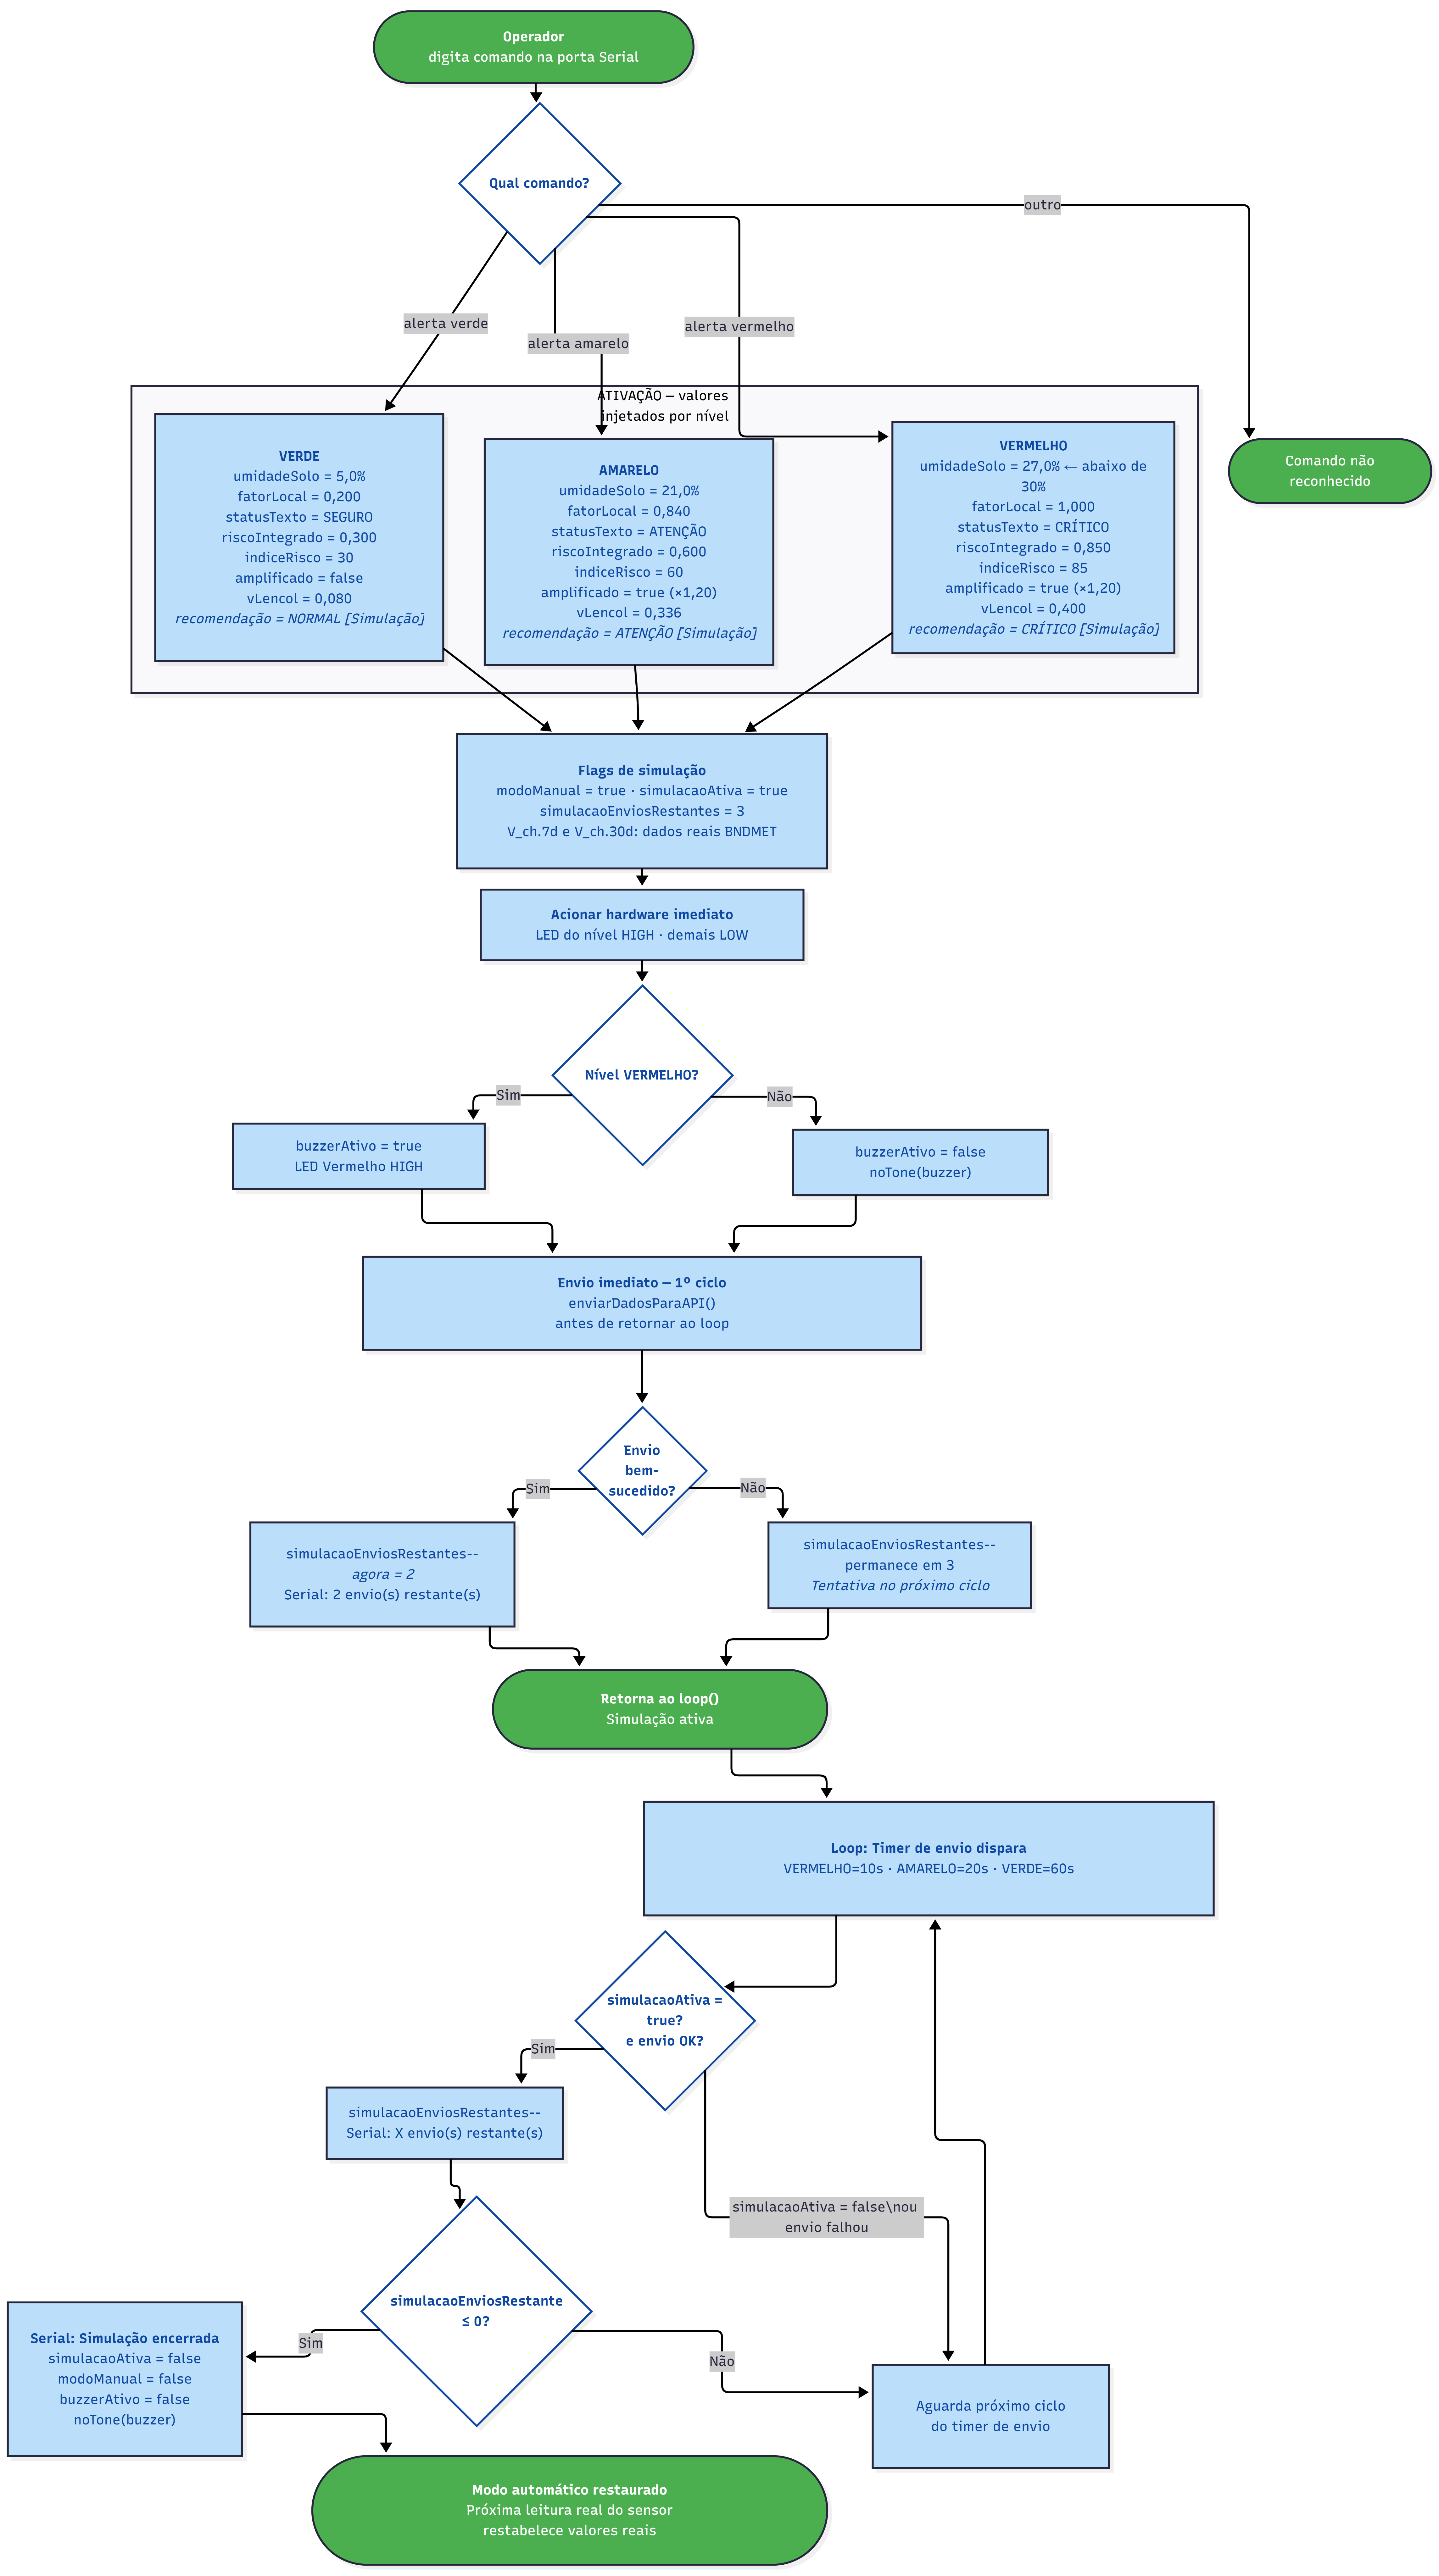
\includegraphics[width=0.85\textwidth]
    {figures/cap4_fluxograma_f9_simulacao_nivel.png}
\caption{Fluxograma do modo de simulação de nível via Serial}
\label{fig:fluxograma_simulacao}
\fonte{Elaborado pela autora.}
\end{figure}

O fluxo tem início com a leitura de um comando na porta Serial.
Os três comandos de simulação disponíveis são \texttt{alerta verde},
\texttt{alerta amarelo} e \texttt{alerta vermelho}; qualquer
outro valor resulta na exibição de mensagem de erro e retorno
ao \textit{loop} sem modificação de estado. Ao reconhecer um
dos três comandos, o \textit{firmware} injeta imediatamente um
conjunto de valores predefinidos nas estruturas
\texttt{DadosLocais} e \texttt{AnaliseRisco}, substituindo os
dados reais do sensor e do modelo de risco pelos valores
representativos do nível solicitado.

Os valores injetados foram definidos para representar cenários
internamente consistentes de cada nível. Para o nível VERDE,
a umidade do solo é fixada em 5,0\%, o fator de risco integrado
em 0,300 e o \textit{status} em ``\textsc{seguro}'', sem
amplificação. Para o nível AMARELO, a umidade é fixada em
21,0\% — posicionando o $F_{len\c{c}ol}$ em 0,840, acima do
limiar de amplificação de 0,70 —, o fator de risco em 0,600 e
o \textit{status} em ``\textsc{atenção}'', com amplificação
ativa. Para o nível VERMELHO, a umidade é fixada
deliberadamente em 27,0\% — três pontos percentuais abaixo do
limiar de ruptura de 30\% —, o fator de risco em 0,850 e o
\textit{status} em ``\textsc{crítico}'', também com amplificação
ativa. O valor de 27,0\% foi escolhido para garantir que o
protocolo de ruptura por \textit{hardware} não seja
inadvertidamente acionado durante a simulação, pois
\texttt{acionarRuptura()} é chamado sempre que a leitura real
do sensor supera 30\%, independentemente do estado de simulação.
Os componentes $V_{ch.7d}$ e $V_{ch.30d}$ não são zerados —
eles utilizam os dados reais do BNDMET já disponíveis em memória,
preservando a coerência meteorológica do registro.

Após a injeção dos valores, três \textit{flags} são ativadas
simultaneamente: \texttt{modoManual = true}, que suspende a
leitura do higrômetro pela função \texttt{atualizarDadosLocais()};
\texttt{simulacaoAtiva = true}, que bloqueia o recálculo da
análise de risco nos dois pontos de guarda do \textit{loop}
(timer de leitura do sensor e timer de análise); e o contador
\texttt{simulacaoEnviosRestantes = 3}, que define quantos
envios bem-sucedidos ao \textit{backend} a simulação realizará
antes de encerrar. Em seguida, o hardware é acionado
imediatamente: o LED correspondente ao nível é ligado, os demais
são desligados, e o \textit{buzzer} é ativado no nível VERMELHO
ou silenciado nos demais com \texttt{noTone()}. Por fim, um
primeiro envio à API é realizado de forma síncrona antes de
retornar ao \textit{loop}, garantindo que pelo menos um registro
seja persistido independentemente do estado do timer de envio.

Durante os ciclos seguintes do \textit{loop}, o timer de envio
continua disparando nos intervalos adaptativos do nível ativo —
10 segundos para VERMELHO, 20 segundos para AMARELO e 60 segundos
para VERDE. A cada envio bem-sucedido com \texttt{simulacaoAtiva
= true}, o contador \texttt{simulacaoEnviosRestantes} é
decrementado. Quando o contador atinge zero, a simulação é
encerrada automaticamente: \texttt{simulacaoAtiva} e
\texttt{modoManual} são desativados, \texttt{buzzerAtivo} é
forçado para \texttt{false} e \texttt{noTone()} é chamado para
garantir silêncio imediato mesmo que o nível simulado fosse
VERMELHO. A mensagem ``\textit{Simulação encerrada — retornando
ao modo automático}'' é exibida na porta Serial. A partir do
próximo ciclo de leitura do sensor, os valores reais do
higrômetro e o ciclo analítico normal são retomados.

% -------------------------------------------------------------
\subsubsubsection{Fluxograma de Envio de Alerta em Massa}
\label{subsubsec:fluxograma-alerta-massa}
% -------------------------------------------------------------

A Figura~\ref{fig:fluxograma_alerta_massa} apresenta o fluxograma
do processo de envio de alerta em massa, acionado pelo Administrador
pela Central de Alertas do painel \textit{web} e processado
integralmente pelo \textit{backend} via \textit{endpoint}
\texttt{POST /auth/enviar-alerta}.

\begin{figure}[htb]
\centering
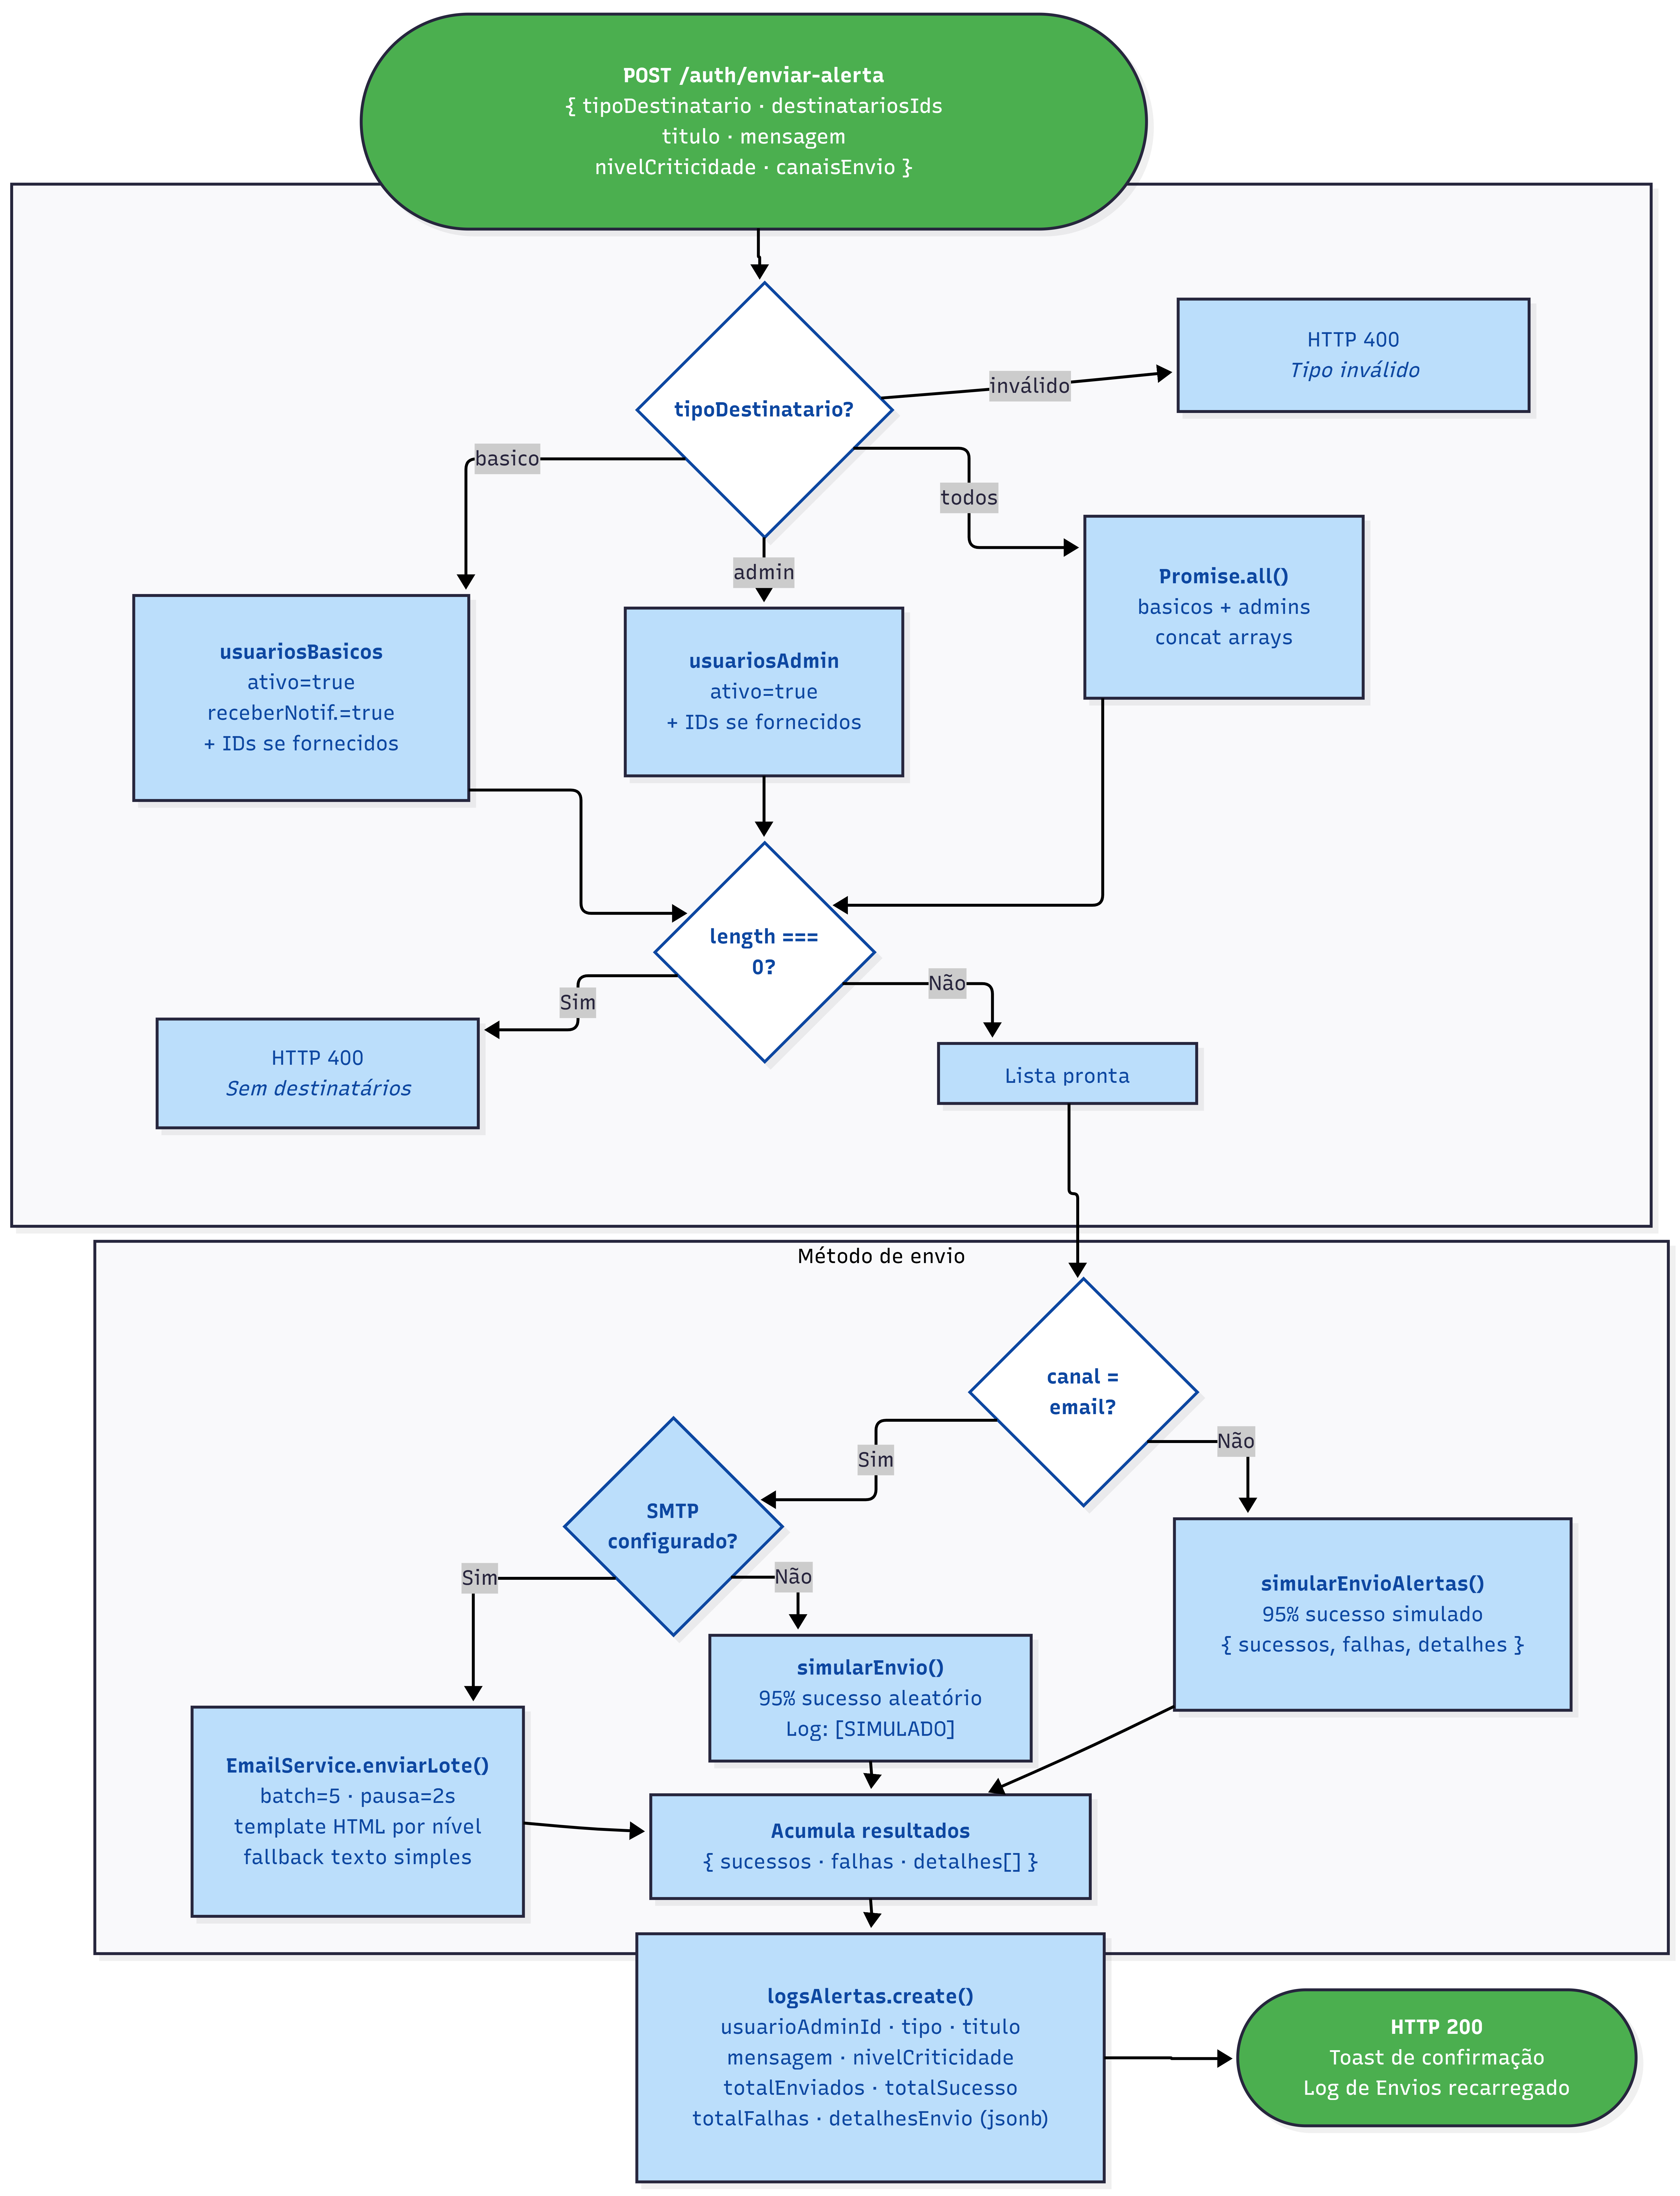
\includegraphics[width=0.95\textwidth]
    {figures/cap4_fluxograma_f10_alerta_massa.png}
\caption{Fluxograma do processo de envio de alerta em massa}
\label{fig:fluxograma_alerta_massa}
\fonte{Elaborado pela autora.}
\end{figure}

O processo tem início com a seleção dos destinatários, determinada
pelo campo \texttt{tipoDestinatario} da requisição. Quando o tipo
é \texttt{basico}, o serviço consulta a tabela
\texttt{usuarios\_basicos} com os filtros \texttt{ativo = true} e
\texttt{receberNotificacoes = true}; quando é \texttt{admin},
consulta \texttt{usuarios\_admin} com \texttt{ativo = true}; quando
é \texttt{todos}, ambas as consultas são executadas em paralelo via
\texttt{Promise.all()} e os resultados são concatenados. Em qualquer
um dos três casos, se o campo \texttt{destinatariosIds} for fornecido
com identificadores não vazios, a consulta é restrita a esses
registros; caso contrário, todos os usuários que atendam aos filtros
são incluídos. Se nenhum destinatário for encontrado para os critérios
informados, o serviço lança uma exceção e retorna
\texttt{HTTP 400} sem processar envios.

Com a lista de destinatários definida, o fluxo avalia dois critérios
independentes para determinar o método de envio. O primeiro critério
é o canal: se \texttt{canaisEnvio} não contém \texttt{'email'} —
cenário de SMS ou \textit{push} —, o serviço chama o método privado
\texttt{simularEnvioAlertas()}, que itera sobre todos os destinatários
e simula uma taxa de sucesso de 95\% por registro, retornando os
totais e o detalhe individual de cada envio. O segundo critério, que
se aplica apenas quando o canal é \texttt{email}, é a disponibilidade
do \textit{transporter} SMTP: se as variáveis de ambiente
\texttt{SMTP\_HOST}, \texttt{SMTP\_USER} e \texttt{SMTP\_PASS}
não estiverem configuradas, o \texttt{EmailService} é inicializado
sem \textit{transporter} e cada chamada a \texttt{enviarAlerta()}
cai automaticamente no método privado \texttt{simularEnvio()}, que
também aplica a taxa de 95\% de sucesso aleatório e registra o evento
no console com o prefixo \texttt{[SIMULADO]}. Quando o SMTP está
disponível, o método \texttt{enviarLote()} processa os destinatários
em grupos de cinco, com pausa de dois segundos entre grupos para
respeitar os limites do servidor de e-mail, e envia para cada
destinatário uma mensagem com \textit{template} HTML colorizado
conforme o nível de criticidade e \textit{fallback} em texto
simples para clientes que não suportam HTML.

Independentemente do método de envio utilizado — SMTP real ou
simulação —, os resultados são acumulados na mesma estrutura
\texttt{\{ sucessos, falhas, detalhes[] \}}, onde \texttt{detalhes}
contém o resultado individual de cada destinatário com
\textit{timestamp}, \textit{status} e mensagem de erro quando
aplicável. Essa estrutura é então persistida na tabela
\texttt{logs\_alertas} via Prisma ORM, com o campo
\texttt{detalhesEnvio} armazenado como \texttt{jsonb} no
PostgreSQL. O registro inclui o identificador do administrador que
disparou o alerta, os totais de sucesso e falha, o nível de
criticidade e o título e mensagem utilizados, constituindo uma
trilha de auditoria completa de todas as notificações enviadas pelo
sistema. O \textit{frontend} exibe o resultado da operação via
\textit{toast} de confirmação e recarrega o modal de Log de Envios
para refletir o novo registro.